\documentclass[twoside]{book}

% Packages required by doxygen
\usepackage{calc}
\usepackage{doxygen}
\usepackage{graphicx}
\usepackage[utf8]{inputenc}
\usepackage{makeidx}
\usepackage{multicol}
\usepackage{multirow}
\usepackage{fixltx2e}
\PassOptionsToPackage{warn}{textcomp}
\usepackage{textcomp}
\usepackage[nointegrals]{wasysym}
\usepackage[table]{xcolor}

% Font selection
\usepackage[T1]{fontenc}
\usepackage{mathptmx}
\usepackage[scaled=.90]{helvet}
\usepackage{courier}
\usepackage{amssymb}
\usepackage{sectsty}
\renewcommand{\familydefault}{\sfdefault}
\allsectionsfont{%
  \fontseries{bc}\selectfont%
  \color{darkgray}%
}
\renewcommand{\DoxyLabelFont}{%
  \fontseries{bc}\selectfont%
  \color{darkgray}%
}
\newcommand{\+}{\discretionary{\mbox{\scriptsize$\hookleftarrow$}}{}{}}

% Page & text layout
\usepackage{geometry}
\geometry{%
  a4paper,%
  top=2.5cm,%
  bottom=2.5cm,%
  left=2.5cm,%
  right=2.5cm%
}
\tolerance=750
\hfuzz=15pt
\hbadness=750
\setlength{\emergencystretch}{15pt}
\setlength{\parindent}{0cm}
\setlength{\parskip}{0.2cm}
\makeatletter
\renewcommand{\paragraph}{%
  \@startsection{paragraph}{4}{0ex}{-1.0ex}{1.0ex}{%
    \normalfont\normalsize\bfseries\SS@parafont%
  }%
}
\renewcommand{\subparagraph}{%
  \@startsection{subparagraph}{5}{0ex}{-1.0ex}{1.0ex}{%
    \normalfont\normalsize\bfseries\SS@subparafont%
  }%
}
\makeatother

% Headers & footers
\usepackage{fancyhdr}
\pagestyle{fancyplain}
\fancyhead[LE]{\fancyplain{}{\bfseries\thepage}}
\fancyhead[CE]{\fancyplain{}{}}
\fancyhead[RE]{\fancyplain{}{\bfseries\leftmark}}
\fancyhead[LO]{\fancyplain{}{\bfseries\rightmark}}
\fancyhead[CO]{\fancyplain{}{}}
\fancyhead[RO]{\fancyplain{}{\bfseries\thepage}}
\fancyfoot[LE]{\fancyplain{}{}}
\fancyfoot[CE]{\fancyplain{}{}}
\fancyfoot[RE]{\fancyplain{}{\bfseries\scriptsize Generated on Wed May 14 2014 17\+:52\+:43 for My Project by Doxygen }}
\fancyfoot[LO]{\fancyplain{}{\bfseries\scriptsize Generated on Wed May 14 2014 17\+:52\+:43 for My Project by Doxygen }}
\fancyfoot[CO]{\fancyplain{}{}}
\fancyfoot[RO]{\fancyplain{}{}}
\renewcommand{\footrulewidth}{0.4pt}
\renewcommand{\chaptermark}[1]{%
  \markboth{#1}{}%
}
\renewcommand{\sectionmark}[1]{%
  \markright{\thesection\ #1}%
}

% Indices & bibliography
\usepackage{natbib}
\usepackage[titles]{tocloft}
\setcounter{tocdepth}{3}
\setcounter{secnumdepth}{5}
\makeindex

% Hyperlinks (required, but should be loaded last)
\usepackage{ifpdf}
\ifpdf
  \usepackage[pdftex,pagebackref=true]{hyperref}
\else
  \usepackage[ps2pdf,pagebackref=true]{hyperref}
\fi
\hypersetup{%
  colorlinks=true,%
  linkcolor=blue,%
  citecolor=blue,%
  unicode%
}

% Custom commands
\newcommand{\clearemptydoublepage}{%
  \newpage{\pagestyle{empty}\cleardoublepage}%
}


%===== C O N T E N T S =====

\begin{document}

% Titlepage & ToC
\hypersetup{pageanchor=false,
             bookmarks=true,
             bookmarksnumbered=true,
             pdfencoding=unicode
            }
\pagenumbering{roman}
\begin{titlepage}
\vspace*{7cm}
\begin{center}%
{\Large My Project }\\
\vspace*{1cm}
{\large Generated by Doxygen 1.8.7}\\
\vspace*{0.5cm}
{\small Wed May 14 2014 17:52:43}\\
\end{center}
\end{titlepage}
\clearemptydoublepage
\tableofcontents
\clearemptydoublepage
\pagenumbering{arabic}
\hypersetup{pageanchor=true}

%--- Begin generated contents ---
\chapter{Hierarchical Index}
\section{Class Hierarchy}
This inheritance list is sorted roughly, but not completely, alphabetically\+:\begin{DoxyCompactList}
\item \contentsline{section}{Attribute}{\pageref{classAttribute}}{}
\item \contentsline{section}{std\+:\+:Constraint}{\pageref{classstd_1_1Constraint}}{}
\item \contentsline{section}{Data}{\pageref{classData}}{}
\item \contentsline{section}{Domain}{\pageref{classDomain}}{}
\item \contentsline{section}{Durative\+Action}{\pageref{classDurativeAction}}{}
\item \contentsline{section}{Edge}{\pageref{classEdge}}{}
\item \contentsline{section}{Fluent}{\pageref{classFluent}}{}
\item \contentsline{section}{Function}{\pageref{classFunction}}{}
\item \contentsline{section}{Graph1}{\pageref{classGraph1}}{}
\item \contentsline{section}{Graph2}{\pageref{classGraph2}}{}
\item \contentsline{section}{Interval}{\pageref{classInterval}}{}
\item \contentsline{section}{Interval\+Agenda}{\pageref{classIntervalAgenda}}{}
\item \contentsline{section}{l\+Obj\+Type}{\pageref{classlObjType}}{}
\item \contentsline{section}{Member}{\pageref{classMember}}{}
\begin{DoxyCompactList}
\item \contentsline{section}{Constant}{\pageref{classConstant}}{}
\item \contentsline{section}{Object}{\pageref{classObject}}{}
\item \contentsline{section}{Variable}{\pageref{classVariable}}{}
\end{DoxyCompactList}
\item \contentsline{section}{Parser\+Base}{\pageref{classParserBase}}{}
\begin{DoxyCompactList}
\item \contentsline{section}{Parser}{\pageref{classParser}}{}
\end{DoxyCompactList}
\item \contentsline{section}{planning\+Data}{\pageref{classplanningData}}{}
\item \contentsline{section}{Predicate}{\pageref{classPredicate}}{}
\item \contentsline{section}{Problem}{\pageref{classProblem}}{}
\item \contentsline{section}{Sat}{\pageref{classSat}}{}
\item \contentsline{section}{Scanner\+Base}{\pageref{classScannerBase}}{}
\begin{DoxyCompactList}
\item \contentsline{section}{Scanner}{\pageref{classScanner}}{}
\end{DoxyCompactList}
\item \contentsline{section}{Scanner\+Base\+:\+:Stream\+Struct}{\pageref{structScannerBase_1_1StreamStruct}}{}
\item \contentsline{section}{Parser\+Base\+:\+:S\+T\+Y\+P\+E\+\_\+\+\_\+}{\pageref{unionParserBase_1_1STYPE____}}{}
\item \contentsline{section}{Tlpgp1}{\pageref{classTlpgp1}}{}
\item \contentsline{section}{Tlpgp2}{\pageref{classTlpgp2}}{}
\item \contentsline{section}{Tools}{\pageref{classTools}}{}
\item \contentsline{section}{Type}{\pageref{classType}}{}
\item \contentsline{section}{Typed\+List}{\pageref{classTypedList}}{}
\item \contentsline{section}{Vertex}{\pageref{classVertex}}{}
\end{DoxyCompactList}

\chapter{Class Index}
\section{Class List}
Here are the classes, structs, unions and interfaces with brief descriptions\+:\begin{DoxyCompactList}
\item\contentsline{section}{\hyperlink{classAttribute}{Attribute} }{\pageref{classAttribute}}{}
\item\contentsline{section}{\hyperlink{classConstant}{Constant} }{\pageref{classConstant}}{}
\item\contentsline{section}{\hyperlink{classstd_1_1Constraint}{std\+::\+Constraint} }{\pageref{classstd_1_1Constraint}}{}
\item\contentsline{section}{\hyperlink{classData}{Data} }{\pageref{classData}}{}
\item\contentsline{section}{\hyperlink{classDomain}{Domain} }{\pageref{classDomain}}{}
\item\contentsline{section}{\hyperlink{classDurativeAction}{Durative\+Action} }{\pageref{classDurativeAction}}{}
\item\contentsline{section}{\hyperlink{classEdge}{Edge} }{\pageref{classEdge}}{}
\item\contentsline{section}{\hyperlink{classFluent}{Fluent} }{\pageref{classFluent}}{}
\item\contentsline{section}{\hyperlink{classFunction}{Function} }{\pageref{classFunction}}{}
\item\contentsline{section}{\hyperlink{classGraph1}{Graph1} }{\pageref{classGraph1}}{}
\item\contentsline{section}{\hyperlink{classGraph2}{Graph2} }{\pageref{classGraph2}}{}
\item\contentsline{section}{\hyperlink{classInterval}{Interval} }{\pageref{classInterval}}{}
\item\contentsline{section}{\hyperlink{classIntervalAgenda}{Interval\+Agenda} }{\pageref{classIntervalAgenda}}{}
\item\contentsline{section}{\hyperlink{classlObjType}{l\+Obj\+Type} }{\pageref{classlObjType}}{}
\item\contentsline{section}{\hyperlink{classMember}{Member} }{\pageref{classMember}}{}
\item\contentsline{section}{\hyperlink{classObject}{Object} }{\pageref{classObject}}{}
\item\contentsline{section}{\hyperlink{classParser}{Parser} }{\pageref{classParser}}{}
\item\contentsline{section}{\hyperlink{classParserBase}{Parser\+Base} }{\pageref{classParserBase}}{}
\item\contentsline{section}{\hyperlink{classplanningData}{planning\+Data} }{\pageref{classplanningData}}{}
\item\contentsline{section}{\hyperlink{classPredicate}{Predicate} }{\pageref{classPredicate}}{}
\item\contentsline{section}{\hyperlink{classProblem}{Problem} }{\pageref{classProblem}}{}
\item\contentsline{section}{\hyperlink{classSat}{Sat} }{\pageref{classSat}}{}
\item\contentsline{section}{\hyperlink{classScanner}{Scanner} }{\pageref{classScanner}}{}
\item\contentsline{section}{\hyperlink{classScannerBase}{Scanner\+Base} }{\pageref{classScannerBase}}{}
\item\contentsline{section}{\hyperlink{structScannerBase_1_1StreamStruct}{Scanner\+Base\+::\+Stream\+Struct} }{\pageref{structScannerBase_1_1StreamStruct}}{}
\item\contentsline{section}{\hyperlink{unionParserBase_1_1STYPE____}{Parser\+Base\+::\+S\+T\+Y\+P\+E\+\_\+\+\_\+} }{\pageref{unionParserBase_1_1STYPE____}}{}
\item\contentsline{section}{\hyperlink{classTlpgp1}{Tlpgp1} }{\pageref{classTlpgp1}}{}
\item\contentsline{section}{\hyperlink{classTlpgp2}{Tlpgp2} }{\pageref{classTlpgp2}}{}
\item\contentsline{section}{\hyperlink{classTools}{Tools} }{\pageref{classTools}}{}
\item\contentsline{section}{\hyperlink{classType}{Type} }{\pageref{classType}}{}
\item\contentsline{section}{\hyperlink{classTypedList}{Typed\+List} }{\pageref{classTypedList}}{}
\item\contentsline{section}{\hyperlink{classVariable}{Variable} }{\pageref{classVariable}}{}
\item\contentsline{section}{\hyperlink{classVertex}{Vertex} }{\pageref{classVertex}}{}
\end{DoxyCompactList}

\chapter{File Index}
\section{File List}
Here is a list of all documented files with brief descriptions\+:\begin{DoxyCompactList}
\item\contentsline{section}{\hyperlink{Data_8cpp}{Data.\+cpp} \\*This class contains the data used by the parser generated with bisonc++ and flexc++ }{\pageref{Data_8cpp}}{}
\item\contentsline{section}{\hyperlink{Data_8h}{Data.\+h} \\*This class contains the data used by the parser generated with bisonc++ and flexc++ }{\pageref{Data_8h}}{}
\item\contentsline{section}{{\bfseries headers.\+h} }{\pageref{headers_8h}}{}
\item\contentsline{section}{\hyperlink{main_8cpp}{main.\+cpp} \\*This program parse P\+D\+D\+L 3.\+1 T\+E domain and problem corresponding file, then it solve the planning problem following T\+L\+P-\/\+G\+P1 and T\+L\+P-\/\+G\+P2 algorithms }{\pageref{main_8cpp}}{}
\item\contentsline{section}{parser/\hyperlink{Parser_8h}{Parser.\+h} \\*This file have been generated by bisonc++ and completed by us }{\pageref{Parser_8h}}{}
\item\contentsline{section}{parser/{\bfseries Parserbase.\+h} }{\pageref{Parserbase_8h}}{}
\item\contentsline{section}{scanner/{\bfseries Scanner.\+h} }{\pageref{Scanner_8h}}{}
\item\contentsline{section}{scanner/{\bfseries Scannerbase.\+h} }{\pageref{Scannerbase_8h}}{}
\item\contentsline{section}{src/\hyperlink{attribute_8cpp}{attribute.\+cpp} \\*This class represent a P\+D\+D\+L Temporally Extended attribute (invented by Frederic Maris), which are the main feature of the interval of preconditions and effects of P\+D\+D\+L durative-\/actions }{\pageref{attribute_8cpp}}{}
\item\contentsline{section}{src/\hyperlink{attribute_8h}{attribute.\+h} \\*This class represent a P\+D\+D\+L Temporally Extended attribute (invented by Frederic Maris), which are the main feature of the interval of preconditions and effects of P\+D\+D\+L durative-\/actions }{\pageref{attribute_8h}}{}
\item\contentsline{section}{src/\hyperlink{constant_8cpp}{constant.\+cpp} \\*This class represent a P\+D\+D\+L constant, inherit from \hyperlink{classMember}{Member} }{\pageref{constant_8cpp}}{}
\item\contentsline{section}{src/\hyperlink{constant_8h}{constant.\+h} \\*This class represent a P\+D\+D\+L constant, inherit from \hyperlink{classMember}{Member} }{\pageref{constant_8h}}{}
\item\contentsline{section}{src/\hyperlink{constraint_8cpp}{constraint.\+cpp} \\*\mbox{[}wip\mbox{]}\mbox{[}test\mbox{]} contains things which may be used in tlpgp1 }{\pageref{constraint_8cpp}}{}
\item\contentsline{section}{src/\hyperlink{constraint_8h}{constraint.\+h} \\*\mbox{[}wip\mbox{]}\mbox{[}test\mbox{]} contains things which may be used in tlpgp1 }{\pageref{constraint_8h}}{}
\item\contentsline{section}{src/{\bfseries domain.\+h} }{\pageref{domain_8h}}{}
\item\contentsline{section}{src/{\bfseries durative\+\_\+action.\+h} }{\pageref{durative__action_8h}}{}
\item\contentsline{section}{src/{\bfseries edge.\+h} }{\pageref{edge_8h}}{}
\item\contentsline{section}{src/\hyperlink{fluent_8cpp}{fluent.\+cpp} \\*This class represent a fluent, which is a predicate of which parameters have been set }{\pageref{fluent_8cpp}}{}
\item\contentsline{section}{src/\hyperlink{fluent_8h}{fluent.\+h} \\*This class represent a fluent, which is a predicate of which parameters have been set }{\pageref{fluent_8h}}{}
\item\contentsline{section}{src/\hyperlink{function_8cpp}{function.\+cpp} \\*This class represent a P\+D\+D\+L function }{\pageref{function_8cpp}}{}
\item\contentsline{section}{src/\hyperlink{function_8h}{function.\+h} \\*This class represent a P\+D\+D\+L function }{\pageref{function_8h}}{}
\item\contentsline{section}{src/{\bfseries graph1.\+h} }{\pageref{graph1_8h}}{}
\item\contentsline{section}{src/\hyperlink{graph2_8cpp}{graph2.\+cpp} \\*Contains what is needed to generate the expansion graph for tlpgp1 }{\pageref{graph2_8cpp}}{}
\item\contentsline{section}{src/\hyperlink{graph2_8h}{graph2.\+h} \\*Contains what is needed to generate the expansion graph for tlpgp1 }{\pageref{graph2_8h}}{}
\item\contentsline{section}{src/\hyperlink{interval_8cpp}{interval.\+cpp} \\*This class represent an interval of which bounds are floats }{\pageref{interval_8cpp}}{}
\item\contentsline{section}{src/\hyperlink{interval_8h}{interval.\+h} \\*This class represent an interval of which bounds are floats }{\pageref{interval_8h}}{}
\item\contentsline{section}{src/\hyperlink{intervalAgenda_8cpp}{interval\+Agenda.\+cpp} \\*The class represents what we will put in the tlpgp1's agenda }{\pageref{intervalAgenda_8cpp}}{}
\item\contentsline{section}{src/\hyperlink{intervalAgenda_8h}{interval\+Agenda.\+h} \\*The class represents what we will put in the tlpgp1's agenda }{\pageref{intervalAgenda_8h}}{}
\item\contentsline{section}{src/{\bfseries l\+Obj\+Type.\+h} }{\pageref{lObjType_8h}}{}
\item\contentsline{section}{src/\hyperlink{member_8cpp}{member.\+cpp} \\*This class represent a P\+D\+D\+L constant, object or variable }{\pageref{member_8cpp}}{}
\item\contentsline{section}{src/\hyperlink{member_8h}{member.\+h} \\*This class represent a P\+D\+D\+L constant, object or variable }{\pageref{member_8h}}{}
\item\contentsline{section}{src/\hyperlink{object_8h}{object.\+h} \\*This class represent a P\+D\+D\+L object, inherit from \hyperlink{classMember}{Member} }{\pageref{object_8h}}{}
\item\contentsline{section}{src/{\bfseries planning\+Data.\+h} }{\pageref{planningData_8h}}{}
\item\contentsline{section}{src/\hyperlink{predicate_8cpp}{predicate.\+cpp} \\*This class represent a P\+D\+D\+L predicate }{\pageref{predicate_8cpp}}{}
\item\contentsline{section}{src/\hyperlink{predicate_8h}{predicate.\+h} \\*This class represent a P\+D\+D\+L predicate }{\pageref{predicate_8h}}{}
\item\contentsline{section}{src/{\bfseries problem.\+h} }{\pageref{problem_8h}}{}
\item\contentsline{section}{src/\hyperlink{sat_8cpp}{sat.\+cpp} \\*What is needed to communicate with a sat solver, using smt2 }{\pageref{sat_8cpp}}{}
\item\contentsline{section}{src/\hyperlink{sat_8h}{sat.\+h} \\*What is needed to communicate with a sat solver, using smt2 }{\pageref{sat_8h}}{}
\item\contentsline{section}{src/\hyperlink{tlpgp1_8cpp}{tlpgp1.\+cpp} \\*\mbox{[}wip\mbox{]}Contains the core code of tlpgp1 }{\pageref{tlpgp1_8cpp}}{}
\item\contentsline{section}{src/\hyperlink{tlpgp1_8h}{tlpgp1.\+h} \\*Contains the core code of tlpgp1 }{\pageref{tlpgp1_8h}}{}
\item\contentsline{section}{src/{\bfseries tlpgp2.\+h} }{\pageref{tlpgp2_8h}}{}
\item\contentsline{section}{src/{\bfseries tools.\+h} }{\pageref{tools_8h}}{}
\item\contentsline{section}{src/\hyperlink{type_8cpp}{type.\+cpp} \\*This class represent a P\+D\+D\+L type }{\pageref{type_8cpp}}{}
\item\contentsline{section}{src/\hyperlink{type_8h}{type.\+h} \\*This class represent a P\+D\+D\+L type }{\pageref{type_8h}}{}
\item\contentsline{section}{src/\hyperlink{typedList_8cpp}{typed\+List.\+cpp} \\*This class represent a parser's typed\+List, which is a pair of a list of name and an either type }{\pageref{typedList_8cpp}}{}
\item\contentsline{section}{src/\hyperlink{typedList_8h}{typed\+List.\+h} \\*This class represent a parser's typed\+List, which is a pair of a list of name and an either type }{\pageref{typedList_8h}}{}
\item\contentsline{section}{src/\hyperlink{variable_8cpp}{variable.\+cpp} \\*This class represent a P\+D\+D\+L variable, inherit from \hyperlink{classMember}{Member} }{\pageref{variable_8cpp}}{}
\item\contentsline{section}{src/\hyperlink{variable_8h}{variable.\+h} \\*This class represent a P\+D\+D\+L variable, inherit from \hyperlink{classMember}{Member} }{\pageref{variable_8h}}{}
\item\contentsline{section}{src/{\bfseries vertex.\+h} }{\pageref{vertex_8h}}{}
\end{DoxyCompactList}

\chapter{Class Documentation}
\hypertarget{classAttribute}{\section{Attribute Class Reference}
\label{classAttribute}\index{Attribute@{Attribute}}
}
\subsection*{Public Member Functions}
\begin{DoxyCompactItemize}
\item 
\hypertarget{classAttribute_a8ba4e5a507aef352563e1e56f1930e66}{\hyperlink{classAttribute_a8ba4e5a507aef352563e1e56f1930e66}{Attribute} ()}\label{classAttribute_a8ba4e5a507aef352563e1e56f1930e66}

\begin{DoxyCompactList}\small\item\em Constructor. \end{DoxyCompactList}\item 
\hypertarget{classAttribute_a28ab087bb886728670e4ae5791bc2ea8}{virtual \hyperlink{classAttribute_a28ab087bb886728670e4ae5791bc2ea8}{$\sim$\+Attribute} ()}\label{classAttribute_a28ab087bb886728670e4ae5791bc2ea8}

\begin{DoxyCompactList}\small\item\em Destructor -\/ virtual. \end{DoxyCompactList}\item 
float \hyperlink{classAttribute_a06d82c170f9a71a4f3925467bcebc824}{get\+Time} ()
\begin{DoxyCompactList}\small\item\em Get the time when occurs the effect (defined with \char`\"{}at\char`\"{}) \end{DoxyCompactList}\item 
void \hyperlink{classAttribute_a14e5f87736aa3520b65fea9867f8faae}{add\+Forbidden} (\hyperlink{classInterval}{Interval} inter)
\begin{DoxyCompactList}\small\item\em Add an interval to the list of interval that are forbidden. \end{DoxyCompactList}\item 
void \hyperlink{classAttribute_a69f34ccca3ff1bb0bb747f869a9b90c6}{add\+Not\+Forbidden} (\hyperlink{classInterval}{Interval} inter)
\begin{DoxyCompactList}\small\item\em Add an interval to the list of interval that are not forbidden. \end{DoxyCompactList}\item 
void \hyperlink{classAttribute_ac4d46fd050a7d9f49eacf697a8f19cb9}{add\+Supported} (\hyperlink{classInterval}{Interval} inter)
\begin{DoxyCompactList}\small\item\em Add an interval to the list of interval that are supported. \end{DoxyCompactList}\item 
void \hyperlink{classAttribute_a285e7380f22708b78c187762319c267b}{add\+Not\+Supported} (\hyperlink{classInterval}{Interval} inter)
\begin{DoxyCompactList}\small\item\em Add an interval to the list of interval that are not supported. \end{DoxyCompactList}\item 
vector$<$ \hyperlink{classInterval}{Interval} $>$ $\ast$ \hyperlink{classAttribute_a22bfaccb31429589929a36244403456e}{get\+Forbidden} ()
\begin{DoxyCompactList}\small\item\em Get the list of interval that are forbidden. \end{DoxyCompactList}\item 
vector$<$ \hyperlink{classInterval}{Interval} $>$ $\ast$ \hyperlink{classAttribute_ad254c796d5ab86a1fdadcb62d464dc4a}{get\+Supported} ()
\begin{DoxyCompactList}\small\item\em Get the list of interval that are supported. \end{DoxyCompactList}\item 
vector$<$ \hyperlink{classInterval}{Interval} $>$ $\ast$ \hyperlink{classAttribute_abd13aeaa71a640c38d20e118c2fb574c}{get\+Not\+Forbidden} ()
\begin{DoxyCompactList}\small\item\em Get the list of interval that are not forbidden. \end{DoxyCompactList}\item 
vector$<$ \hyperlink{classInterval}{Interval} $>$ $\ast$ \hyperlink{classAttribute_a5885a1bf4129cde5e8e7b55d46fd7cda}{get\+Not\+Supported} ()
\begin{DoxyCompactList}\small\item\em Get the list of interval that are not supported. \end{DoxyCompactList}\item 
string \hyperlink{classAttribute_a9701171d288a295393e48eb767564a53}{to\+\_\+string} ()
\begin{DoxyCompactList}\small\item\em Return a string that represent the attribute. \end{DoxyCompactList}\end{DoxyCompactItemize}


\subsection{Member Function Documentation}
\hypertarget{classAttribute_a14e5f87736aa3520b65fea9867f8faae}{\index{Attribute@{Attribute}!add\+Forbidden@{add\+Forbidden}}
\index{add\+Forbidden@{add\+Forbidden}!Attribute@{Attribute}}
\subsubsection[{add\+Forbidden}]{\setlength{\rightskip}{0pt plus 5cm}void Attribute\+::add\+Forbidden (
\begin{DoxyParamCaption}
\item[{{\bf Interval}}]{inter}
\end{DoxyParamCaption}
)}}\label{classAttribute_a14e5f87736aa3520b65fea9867f8faae}


Add an interval to the list of interval that are forbidden. 


\begin{DoxyParams}{Parameters}
{\em inter} & -\/ the new interval to add in m\+\_\+forbidden \\
\hline
\end{DoxyParams}
\hypertarget{classAttribute_a69f34ccca3ff1bb0bb747f869a9b90c6}{\index{Attribute@{Attribute}!add\+Not\+Forbidden@{add\+Not\+Forbidden}}
\index{add\+Not\+Forbidden@{add\+Not\+Forbidden}!Attribute@{Attribute}}
\subsubsection[{add\+Not\+Forbidden}]{\setlength{\rightskip}{0pt plus 5cm}void Attribute\+::add\+Not\+Forbidden (
\begin{DoxyParamCaption}
\item[{{\bf Interval}}]{inter}
\end{DoxyParamCaption}
)}}\label{classAttribute_a69f34ccca3ff1bb0bb747f869a9b90c6}


Add an interval to the list of interval that are not forbidden. 


\begin{DoxyParams}{Parameters}
{\em inter} & -\/ the new interval to add in m\+\_\+not\+\_\+forbidden \\
\hline
\end{DoxyParams}
\hypertarget{classAttribute_a285e7380f22708b78c187762319c267b}{\index{Attribute@{Attribute}!add\+Not\+Supported@{add\+Not\+Supported}}
\index{add\+Not\+Supported@{add\+Not\+Supported}!Attribute@{Attribute}}
\subsubsection[{add\+Not\+Supported}]{\setlength{\rightskip}{0pt plus 5cm}void Attribute\+::add\+Not\+Supported (
\begin{DoxyParamCaption}
\item[{{\bf Interval}}]{inter}
\end{DoxyParamCaption}
)}}\label{classAttribute_a285e7380f22708b78c187762319c267b}


Add an interval to the list of interval that are not supported. 


\begin{DoxyParams}{Parameters}
{\em inter} & -\/ the new interval to add in m\+\_\+not\+\_\+supported \\
\hline
\end{DoxyParams}
\hypertarget{classAttribute_ac4d46fd050a7d9f49eacf697a8f19cb9}{\index{Attribute@{Attribute}!add\+Supported@{add\+Supported}}
\index{add\+Supported@{add\+Supported}!Attribute@{Attribute}}
\subsubsection[{add\+Supported}]{\setlength{\rightskip}{0pt plus 5cm}void Attribute\+::add\+Supported (
\begin{DoxyParamCaption}
\item[{{\bf Interval}}]{inter}
\end{DoxyParamCaption}
)}}\label{classAttribute_ac4d46fd050a7d9f49eacf697a8f19cb9}


Add an interval to the list of interval that are supported. 


\begin{DoxyParams}{Parameters}
{\em inter} & -\/ the new interval to add in m\+\_\+supported \\
\hline
\end{DoxyParams}
\hypertarget{classAttribute_a22bfaccb31429589929a36244403456e}{\index{Attribute@{Attribute}!get\+Forbidden@{get\+Forbidden}}
\index{get\+Forbidden@{get\+Forbidden}!Attribute@{Attribute}}
\subsubsection[{get\+Forbidden}]{\setlength{\rightskip}{0pt plus 5cm}vector$<$ {\bf Interval} $>$ $\ast$ Attribute\+::get\+Forbidden (
\begin{DoxyParamCaption}
{}
\end{DoxyParamCaption}
)}}\label{classAttribute_a22bfaccb31429589929a36244403456e}


Get the list of interval that are forbidden. 

\begin{DoxyReturn}{Returns}
a pointer to m\+\_\+forbidden 
\end{DoxyReturn}
\hypertarget{classAttribute_abd13aeaa71a640c38d20e118c2fb574c}{\index{Attribute@{Attribute}!get\+Not\+Forbidden@{get\+Not\+Forbidden}}
\index{get\+Not\+Forbidden@{get\+Not\+Forbidden}!Attribute@{Attribute}}
\subsubsection[{get\+Not\+Forbidden}]{\setlength{\rightskip}{0pt plus 5cm}vector$<$ {\bf Interval} $>$ $\ast$ Attribute\+::get\+Not\+Forbidden (
\begin{DoxyParamCaption}
{}
\end{DoxyParamCaption}
)}}\label{classAttribute_abd13aeaa71a640c38d20e118c2fb574c}


Get the list of interval that are not forbidden. 

\begin{DoxyReturn}{Returns}
a pointer to m\+\_\+not\+\_\+forbidden 
\end{DoxyReturn}
\hypertarget{classAttribute_a5885a1bf4129cde5e8e7b55d46fd7cda}{\index{Attribute@{Attribute}!get\+Not\+Supported@{get\+Not\+Supported}}
\index{get\+Not\+Supported@{get\+Not\+Supported}!Attribute@{Attribute}}
\subsubsection[{get\+Not\+Supported}]{\setlength{\rightskip}{0pt plus 5cm}vector$<$ {\bf Interval} $>$ $\ast$ Attribute\+::get\+Not\+Supported (
\begin{DoxyParamCaption}
{}
\end{DoxyParamCaption}
)}}\label{classAttribute_a5885a1bf4129cde5e8e7b55d46fd7cda}


Get the list of interval that are not supported. 

\begin{DoxyReturn}{Returns}
a pointer to m\+\_\+not\+\_\+supported 
\end{DoxyReturn}
\hypertarget{classAttribute_ad254c796d5ab86a1fdadcb62d464dc4a}{\index{Attribute@{Attribute}!get\+Supported@{get\+Supported}}
\index{get\+Supported@{get\+Supported}!Attribute@{Attribute}}
\subsubsection[{get\+Supported}]{\setlength{\rightskip}{0pt plus 5cm}vector$<$ {\bf Interval} $>$ $\ast$ Attribute\+::get\+Supported (
\begin{DoxyParamCaption}
{}
\end{DoxyParamCaption}
)}}\label{classAttribute_ad254c796d5ab86a1fdadcb62d464dc4a}


Get the list of interval that are supported. 

\begin{DoxyReturn}{Returns}
a pointer to m\+\_\+supported 
\end{DoxyReturn}
\hypertarget{classAttribute_a06d82c170f9a71a4f3925467bcebc824}{\index{Attribute@{Attribute}!get\+Time@{get\+Time}}
\index{get\+Time@{get\+Time}!Attribute@{Attribute}}
\subsubsection[{get\+Time}]{\setlength{\rightskip}{0pt plus 5cm}float Attribute\+::get\+Time (
\begin{DoxyParamCaption}
{}
\end{DoxyParamCaption}
)}}\label{classAttribute_a06d82c170f9a71a4f3925467bcebc824}


Get the time when occurs the effect (defined with \char`\"{}at\char`\"{}) 

\begin{DoxyReturn}{Returns}
0 if the effect occurs at the beginning of the action, else the duration of the action 
\end{DoxyReturn}
\hypertarget{classAttribute_a9701171d288a295393e48eb767564a53}{\index{Attribute@{Attribute}!to\+\_\+string@{to\+\_\+string}}
\index{to\+\_\+string@{to\+\_\+string}!Attribute@{Attribute}}
\subsubsection[{to\+\_\+string}]{\setlength{\rightskip}{0pt plus 5cm}string Attribute\+::to\+\_\+string (
\begin{DoxyParamCaption}
{}
\end{DoxyParamCaption}
)}}\label{classAttribute_a9701171d288a295393e48eb767564a53}


Return a string that represent the attribute. 

\begin{DoxyReturn}{Returns}
a string \char`\"{}\mbox{[}forbidden on m\+\_\+forbidden\mbox{]} \mbox{[}supported on m\+\_\+supported\mbox{]} \mbox{[}not forbidden on m\+\_\+not\+\_\+forbidden\mbox{]} \mbox{[}not supported on m\+\_\+not\+\_\+supported\mbox{]}\char`\"{} 
\end{DoxyReturn}


The documentation for this class was generated from the following files\+:\begin{DoxyCompactItemize}
\item 
src/\hyperlink{attribute_8h}{attribute.\+h}\item 
src/\hyperlink{attribute_8cpp}{attribute.\+cpp}\end{DoxyCompactItemize}

\hypertarget{classConstant}{\section{Constant Class Reference}
\label{classConstant}\index{Constant@{Constant}}
}
Inheritance diagram for Constant\+:\begin{figure}[H]
\begin{center}
\leavevmode
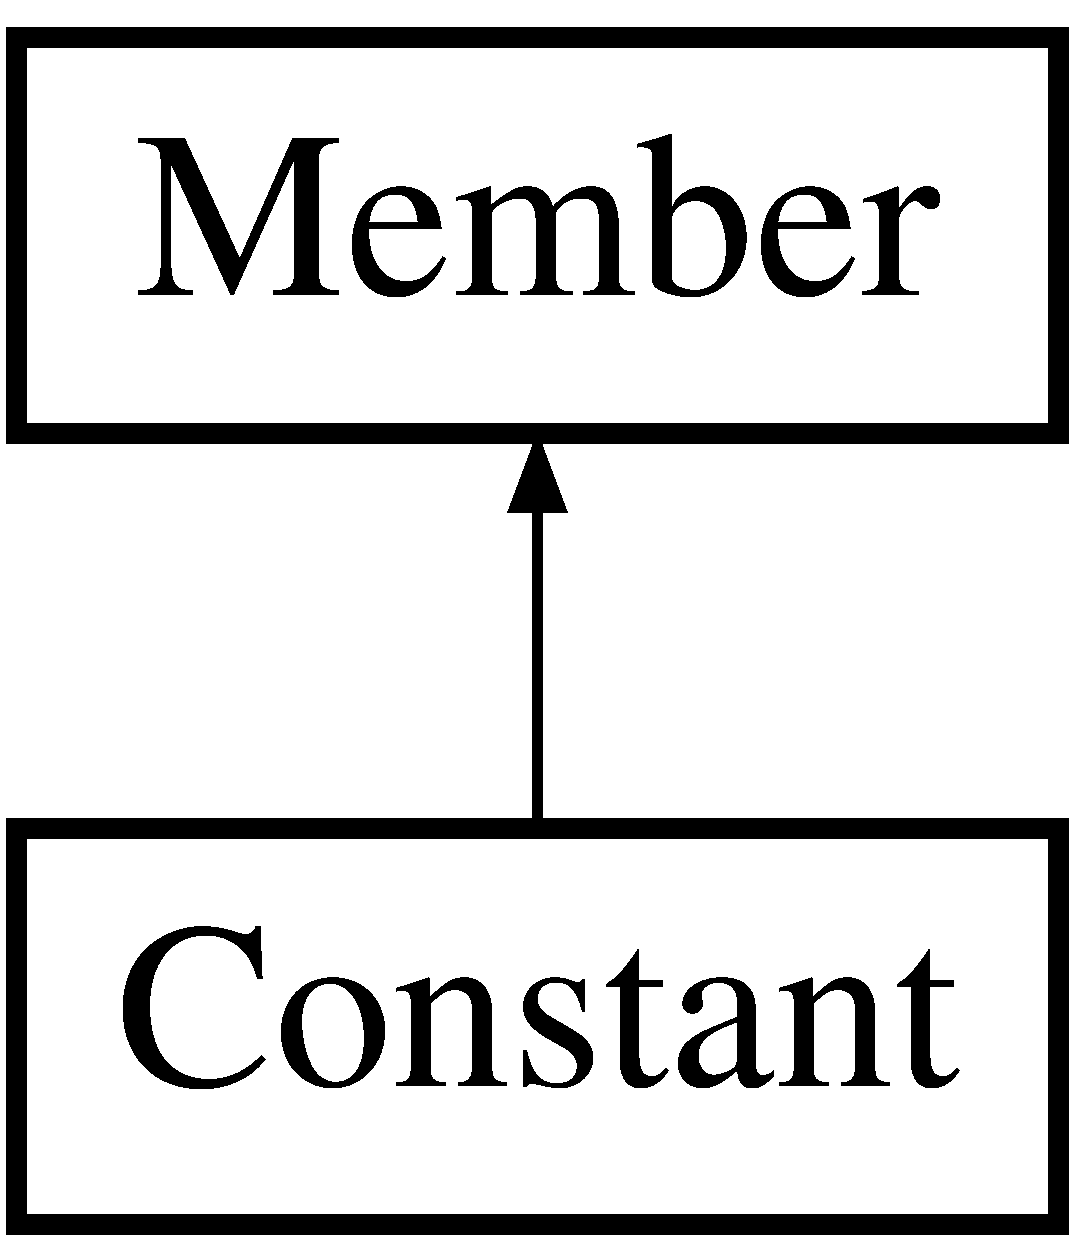
\includegraphics[height=2.000000cm]{classConstant}
\end{center}
\end{figure}
\subsection*{Public Member Functions}
\begin{DoxyCompactItemize}
\item 
\hypertarget{classConstant_a6d2f7d070d22aed4a3371c181da67716}{\hyperlink{classConstant_a6d2f7d070d22aed4a3371c181da67716}{Constant} ()}\label{classConstant_a6d2f7d070d22aed4a3371c181da67716}

\begin{DoxyCompactList}\small\item\em Constructor. \end{DoxyCompactList}\item 
\hyperlink{classConstant_a0d9865c2d8d7f2a81b3048b694806534}{Constant} (string name, vector$<$ \hyperlink{classType}{Type} $\ast$ $>$ types)
\begin{DoxyCompactList}\small\item\em Constructor. \end{DoxyCompactList}\item 
void \hyperlink{classConstant_ac94ccf014f636837cf0be22a227fe1c8}{add\+Types} (vector$<$ \hyperlink{classType}{Type} $\ast$ $>$ types)
\begin{DoxyCompactList}\small\item\em Add an either type to the existing either type of the constant (doesn't duplicate) \end{DoxyCompactList}\item 
string \hyperlink{classConstant_a685a4dbdc864e61c3e14a0fd974ba024}{to\+\_\+string} ()
\begin{DoxyCompactList}\small\item\em Return a string that represent the constant. \end{DoxyCompactList}\item 
string \hyperlink{classConstant_aeb11c90406eb42af86ba8898fb774e1d}{get\+Class} ()
\begin{DoxyCompactList}\small\item\em Return the name of the class. \end{DoxyCompactList}\end{DoxyCompactItemize}
\subsection*{Additional Inherited Members}


\subsection{Constructor \& Destructor Documentation}
\hypertarget{classConstant_a0d9865c2d8d7f2a81b3048b694806534}{\index{Constant@{Constant}!Constant@{Constant}}
\index{Constant@{Constant}!Constant@{Constant}}
\subsubsection[{Constant}]{\setlength{\rightskip}{0pt plus 5cm}Constant\+::\+Constant (
\begin{DoxyParamCaption}
\item[{string}]{name, }
\item[{vector$<$ {\bf Type} $\ast$ $>$}]{types}
\end{DoxyParamCaption}
)}}\label{classConstant_a0d9865c2d8d7f2a81b3048b694806534}


Constructor. 


\begin{DoxyParams}{Parameters}
{\em name} & -\/ name of the constant types -\/ either type of the constant \\
\hline
\end{DoxyParams}


\subsection{Member Function Documentation}
\hypertarget{classConstant_ac94ccf014f636837cf0be22a227fe1c8}{\index{Constant@{Constant}!add\+Types@{add\+Types}}
\index{add\+Types@{add\+Types}!Constant@{Constant}}
\subsubsection[{add\+Types}]{\setlength{\rightskip}{0pt plus 5cm}void Constant\+::add\+Types (
\begin{DoxyParamCaption}
\item[{vector$<$ {\bf Type} $\ast$ $>$}]{types}
\end{DoxyParamCaption}
)}}\label{classConstant_ac94ccf014f636837cf0be22a227fe1c8}


Add an either type to the existing either type of the constant (doesn't duplicate) 


\begin{DoxyParams}{Parameters}
{\em types} & -\/ either type to add to the constant \\
\hline
\end{DoxyParams}
\hypertarget{classConstant_aeb11c90406eb42af86ba8898fb774e1d}{\index{Constant@{Constant}!get\+Class@{get\+Class}}
\index{get\+Class@{get\+Class}!Constant@{Constant}}
\subsubsection[{get\+Class}]{\setlength{\rightskip}{0pt plus 5cm}string Constant\+::get\+Class (
\begin{DoxyParamCaption}
{}
\end{DoxyParamCaption}
)\hspace{0.3cm}{\ttfamily [virtual]}}}\label{classConstant_aeb11c90406eb42af86ba8898fb774e1d}


Return the name of the class. 

\begin{DoxyReturn}{Returns}
\char`\"{}\+Constant\char`\"{} 
\end{DoxyReturn}


Reimplemented from \hyperlink{classMember_a7178ead1b2f1daa5fc5f993281ec90a4}{Member}.

\hypertarget{classConstant_a685a4dbdc864e61c3e14a0fd974ba024}{\index{Constant@{Constant}!to\+\_\+string@{to\+\_\+string}}
\index{to\+\_\+string@{to\+\_\+string}!Constant@{Constant}}
\subsubsection[{to\+\_\+string}]{\setlength{\rightskip}{0pt plus 5cm}string Constant\+::to\+\_\+string (
\begin{DoxyParamCaption}
{}
\end{DoxyParamCaption}
)\hspace{0.3cm}{\ttfamily [virtual]}}}\label{classConstant_a685a4dbdc864e61c3e14a0fd974ba024}


Return a string that represent the constant. 

\begin{DoxyReturn}{Returns}
a string \char`\"{}\+Constant name -\/ either type\char`\"{} 
\end{DoxyReturn}


Reimplemented from \hyperlink{classMember_aaa0028059dd87706188ee670bd28e4f2}{Member}.



The documentation for this class was generated from the following files\+:\begin{DoxyCompactItemize}
\item 
src/\hyperlink{constant_8h}{constant.\+h}\item 
src/\hyperlink{constant_8cpp}{constant.\+cpp}\end{DoxyCompactItemize}

\hypertarget{classstd_1_1constraint}{\section{std\+:\+:constraint Class Reference}
\label{classstd_1_1constraint}\index{std\+::constraint@{std\+::constraint}}
}
\subsection*{Public Member Functions}
\begin{DoxyCompactItemize}
\item 
\hypertarget{classstd_1_1constraint_ab4b674cced2902e04f0dd6d7be7d0e13}{{\bfseries constraint} (int time\+Left, int time\+Right, string comparison, \hyperlink{classDurativeAction}{Durative\+Action} $\ast$action\+Left, \hyperlink{classDurativeAction}{Durative\+Action} $\ast$action\+Right)}\label{classstd_1_1constraint_ab4b674cced2902e04f0dd6d7be7d0e13}

\item 
\hypertarget{classstd_1_1constraint_a5efebbd0b796484d032c69dc11807919}{void {\bfseries print} ()}\label{classstd_1_1constraint_a5efebbd0b796484d032c69dc11807919}

\end{DoxyCompactItemize}


The documentation for this class was generated from the following files\+:\begin{DoxyCompactItemize}
\item 
src/\hyperlink{constraint_8h}{constraint.\+h}\item 
src/\hyperlink{constraint_8cpp}{constraint.\+cpp}\end{DoxyCompactItemize}

\hypertarget{classData}{\section{Data Class Reference}
\label{classData}\index{Data@{Data}}
}
\subsection*{Public Member Functions}
\begin{DoxyCompactItemize}
\item 
\hypertarget{classData_af11f741cb7f587e2e495452a8905a22a}{\hyperlink{classData_af11f741cb7f587e2e495452a8905a22a}{Data} ()}\label{classData_af11f741cb7f587e2e495452a8905a22a}

\begin{DoxyCompactList}\small\item\em Constructor. \end{DoxyCompactList}\item 
\hypertarget{classData_aab31956423290f0d62dcca47ab4d16dd}{virtual \hyperlink{classData_aab31956423290f0d62dcca47ab4d16dd}{$\sim$\+Data} ()}\label{classData_aab31956423290f0d62dcca47ab4d16dd}

\begin{DoxyCompactList}\small\item\em Destructor. \end{DoxyCompactList}\item 
void \hyperlink{classData_adcab26af5124ec74d78fe287d5fe230b}{add\+Domain} (string $\ast$name)
\begin{DoxyCompactList}\small\item\em Set the name of the domain. \end{DoxyCompactList}\item 
\hyperlink{classDomain}{Domain} $\ast$ \hyperlink{classData_ab089c7118ff881bb68aea9219bf3ce71}{get\+Domain} ()
\begin{DoxyCompactList}\small\item\em Create a pointer to the domain. \end{DoxyCompactList}\item 
\hyperlink{classProblem}{Problem} $\ast$ \hyperlink{classData_aec1aab3dbf34f208145f9a5998b0361a}{get\+Problem} ()
\begin{DoxyCompactList}\small\item\em Create a pointer to the problem. \end{DoxyCompactList}\item 
bool \hyperlink{classData_ab1bf9174e79a11a839b4c20638e900b4}{is\+Domain} (string $\ast$name)
\begin{DoxyCompactList}\small\item\em Verify if name is the name of the domain previously parsed. \end{DoxyCompactList}\item 
bool \hyperlink{classData_ab7776fd08b027d7fe13aef078074c1c3}{add\+Requirement} (int req)
\begin{DoxyCompactList}\small\item\em Add the requirement req in m\+\_\+requirement once read in \+:requirements. \end{DoxyCompactList}\item 
bool \hyperlink{classData_a7b65c60ee62668bac343e4d375f5e6d0}{is\+Requirement} (int req)
\begin{DoxyCompactList}\small\item\em Verify if the requirement req has been announced in \+:requirements, and stored in m\+\_\+requirements. \end{DoxyCompactList}\item 
bool \hyperlink{classData_a7ad500e35daba61a234d65036b313daf}{add\+Types} (std\+::vector$<$ \hyperlink{classTypedList}{Typed\+List} $\ast$ $>$ $\ast$typed\+List\+\_\+list)
\begin{DoxyCompactList}\small\item\em Add the types in m\+\_\+types once read in \+:types and add the name of this type in m\+\_\+type\+\_\+list. \end{DoxyCompactList}\item 
bool \hyperlink{classData_abef55e0e00df2b789f477a17f1f0f49b}{is\+Type} (string type)
\begin{DoxyCompactList}\small\item\em Verify if the type type has been defined, in m\+\_\+type\+\_\+list. \end{DoxyCompactList}\item 
\hyperlink{classType}{Type} $\ast$ \hyperlink{classData_abf4f2b05619ed894c0541c9f26cba194}{get\+Type} (string name)
\begin{DoxyCompactList}\small\item\em Get the pointer to a type contained in m\+\_\+types. \end{DoxyCompactList}\item 
bool \hyperlink{classData_af7e7c80360098609c34d5eb1e2947f34}{add\+Constants} (vector$<$ \hyperlink{classTypedList}{Typed\+List} $\ast$ $>$ $\ast$typed\+List\+\_\+list)
\begin{DoxyCompactList}\small\item\em Add the constants in m\+\_\+constants once read in \+:constants and add the name of this constant in m\+\_\+constant\+\_\+list. \end{DoxyCompactList}\item 
bool \hyperlink{classData_a970cb780e68756fffeab7539712bae08}{is\+Constant} (string constant)
\begin{DoxyCompactList}\small\item\em Verify if the constant constant has been defined, in m\+\_\+constant\+\_\+list. \end{DoxyCompactList}\item 
\hyperlink{classConstant}{Constant} $\ast$ \hyperlink{classData_a642f5f3f6735c2b5845ba2c151b79b1f}{get\+Constant} (string constant)
\begin{DoxyCompactList}\small\item\em Get the pointer to a constant contained in m\+\_\+constants. \end{DoxyCompactList}\item 
bool \hyperlink{classData_a8d3815b9c9f97e6fef596c431af7dd39}{add\+Predicate} (string $\ast$name, vector$<$ \hyperlink{classTypedList}{Typed\+List} $\ast$ $>$ $\ast$typed\+List\+\_\+list)
\begin{DoxyCompactList}\small\item\em Add the predicates in m\+\_\+predicates once read in \+:predicates. \end{DoxyCompactList}\item 
bool \hyperlink{classData_a8b38b503a1026118a9dde08be92f609f}{is\+Predicate} (string $\ast$name, vector$<$ \hyperlink{classTypedList}{Typed\+List} $\ast$ $>$ $\ast$typed\+List\+\_\+list)
\begin{DoxyCompactList}\small\item\em Verify if the predicate have been defined in m\+\_\+predicates. \end{DoxyCompactList}\item 
bool \hyperlink{classData_a5b576ebad8f95406f9940e832b401d45}{is\+Predicate} (string $\ast$name, vector$<$ vector$<$ \hyperlink{classType}{Type} $\ast$ $>$ $>$ types)
\begin{DoxyCompactList}\small\item\em Verify if the predicate have been defined in m\+\_\+predicates. \end{DoxyCompactList}\item 
\hyperlink{classPredicate}{Predicate} $\ast$ \hyperlink{classData_a639f1aec2b6917247a9835907a638c52}{get\+Predicate} (string $\ast$name, vector$<$ vector$<$ \hyperlink{classType}{Type} $\ast$ $>$ $>$ types)
\begin{DoxyCompactList}\small\item\em Get the pointer to a predicate contained in m\+\_\+predicates. \end{DoxyCompactList}\item 
bool \hyperlink{classData_af1c23bcc960f630dd922a2b7536f3976}{add\+Functions} (vector$<$ pair$<$ string $\ast$, vector$<$ \hyperlink{classTypedList}{Typed\+List} $\ast$ $>$ $\ast$ $>$ $\ast$ $>$ $\ast$function\+\_\+skeleton\+\_\+list, vector$<$ string $>$ $\ast$return\+\_\+type)
\begin{DoxyCompactList}\small\item\em Add the functions in m\+\_\+functions once read in \+:functions. \end{DoxyCompactList}\item 
bool \hyperlink{classData_ab6d02279beb84726bb046dadf8190222}{add\+Function} (string $\ast$name, vector$<$ \hyperlink{classType}{Type} $\ast$ $>$ return\+\_\+type, vector$<$ \hyperlink{classTypedList}{Typed\+List} $\ast$ $>$ $\ast$typed\+List\+\_\+list)
\begin{DoxyCompactList}\small\item\em Add one function in m\+\_\+functions. \end{DoxyCompactList}\item 
bool \hyperlink{classData_a62ef476f066455ffd3e5d9f2ffde145f}{is\+Function} (string $\ast$name, vector$<$ \hyperlink{classTypedList}{Typed\+List} $\ast$ $>$ $\ast$typed\+List\+\_\+list)
\begin{DoxyCompactList}\small\item\em Verify if the function have been defined in m\+\_\+functions. \end{DoxyCompactList}\item 
void \hyperlink{classData_a4ef55d895e6eefe77091a154edf4614d}{add\+Problem} (string $\ast$name)
\begin{DoxyCompactList}\small\item\em Set the name of the problem. \end{DoxyCompactList}\item 
bool \hyperlink{classData_af3f253e6aac97be58347b71b977dab83}{add\+Objects} (vector$<$ \hyperlink{classTypedList}{Typed\+List} $\ast$ $>$ $\ast$typed\+List\+\_\+list)
\begin{DoxyCompactList}\small\item\em Add the objects in m\+\_\+objects once read in \+:objects and add the name of this object in m\+\_\+object\+\_\+list. \end{DoxyCompactList}\item 
bool \hyperlink{classData_a850db73b9a3cfada1e204853a66222dd}{is\+Object} (string object)
\begin{DoxyCompactList}\small\item\em Verify if the object object has been defined, in m\+\_\+object\+\_\+list. \end{DoxyCompactList}\item 
\hyperlink{classObject}{Object} $\ast$ \hyperlink{classData_a7e021783ede1baa1bfea1023d181755f}{get\+Object} (string object)
\begin{DoxyCompactList}\small\item\em Get the pointer to a object contained in m\+\_\+objects. \end{DoxyCompactList}\item 
bool \hyperlink{classData_a27908a242e9862807ee0ab5cb0fd26de}{add\+Init} (pair$<$ pair$<$ vector$<$ string $>$ $\ast$, string $\ast$ $>$ $\ast$, bool $>$ $\ast$literal, float at)
\begin{DoxyCompactList}\small\item\em Add an init fluent in m\+\_\+inits once read in \+:init. \end{DoxyCompactList}\item 
vector$<$ pair$<$ \hyperlink{classFluent}{Fluent} \\*
$\ast$, \hyperlink{classAttribute}{Attribute} $>$ $>$ $\ast$ \hyperlink{classData_a915f723d120af4837bd5746791bfdc8a}{get\+Inits} ()
\begin{DoxyCompactList}\small\item\em Get a pointer to the list m\+\_\+inits. \end{DoxyCompactList}\item 
bool \hyperlink{classData_add87185f44e1d804657c0eebeaf8ae2c}{add\+Goals} (vector$<$ vector$<$ pair$<$ pair$<$ vector$<$ string $>$ $\ast$, string $\ast$ $>$ $\ast$, int $>$ $\ast$ $>$ $\ast$ $>$ $\ast$pre\+\_\+\+G\+D)
\begin{DoxyCompactList}\small\item\em Add the goal fluents in m\+\_\+goals once read in \+:goal. \end{DoxyCompactList}\item 
vector$<$ pair$<$ \hyperlink{classFluent}{Fluent} \\*
$\ast$, \hyperlink{classAttribute}{Attribute} $>$ $>$ $\ast$ \hyperlink{classData_a631b33415dab9a790804d289bc28ecbc}{get\+Goals} ()
\begin{DoxyCompactList}\small\item\em Get a pointer to the list m\+\_\+goals. \end{DoxyCompactList}\item 
bool \hyperlink{classData_a45b34ea5c6736c80751955960bca0ffe}{is\+Action} (string const $\ast$name)
\begin{DoxyCompactList}\small\item\em Verify if the durative-\/action name has been defined, in m\+\_\+actions. \end{DoxyCompactList}\item 
vector$<$ \hyperlink{classDurativeAction}{Durative\+Action} $\ast$ $>$ $\ast$ \hyperlink{classData_a240c4f180de6fecdc27828f7372bc097}{get\+Actions} ()
\begin{DoxyCompactList}\small\item\em Get a pointer to the list m\+\_\+actions. \end{DoxyCompactList}\item 
\hypertarget{classData_a636be6b2bdfbdc7c7443f8ec8f355050}{void \hyperlink{classData_a636be6b2bdfbdc7c7443f8ec8f355050}{display} ()}\label{classData_a636be6b2bdfbdc7c7443f8ec8f355050}

\begin{DoxyCompactList}\small\item\em Display the data (domain variables, problem variables, and errors) in stdout. \end{DoxyCompactList}\item 
void \hyperlink{classData_ac0f3cb4edd016d70b6e1510c7d5be6eb}{lexical\+\_\+error} (string msg)
\begin{DoxyCompactList}\small\item\em Add a warning in the list m\+\_\+errors. \end{DoxyCompactList}\item 
void \hyperlink{classData_aabe4046094f2f22776988fe24a174065}{fatal\+\_\+error} (string msg)
\begin{DoxyCompactList}\small\item\em Stop the execution and print the error message on stderr. \end{DoxyCompactList}\item 
bool \hyperlink{classData_a9683ed950f2f4417f52abdfead47224c}{add\+Durative\+Action} (string $\ast$name, vector$<$ \hyperlink{classTypedList}{Typed\+List} $\ast$ $>$ $\ast$typed\+List\+\_\+list, float number, vector$<$ pair$<$ pair$<$ vector$<$ string $>$ $\ast$, string $\ast$ $>$ $\ast$, int $>$ $\ast$ $>$ $\ast$timed\+\_\+\+G\+D, vector$<$ pair$<$ pair$<$ vector$<$ string $>$ $\ast$, string $\ast$ $>$ $\ast$, int $>$ $\ast$ $>$ $\ast$cond\+\_\+effect)
\begin{DoxyCompactList}\small\item\em Add adurative-\/action in m\+\_\+actions once read in \+:durative-\/action. \end{DoxyCompactList}\item 
bool \hyperlink{classData_a54b144fea33e662b4f2e461b9c741079}{add\+Initiated\+Function} (pair$<$ vector$<$ string $>$ $\ast$, string $\ast$ $>$ $\ast$atomic\+\_\+formula, float number)
\begin{DoxyCompactList}\small\item\em Add an initiated function in m\+\_\+initiated\+\_\+functions once read in \+:init. \end{DoxyCompactList}\item 
bool \hyperlink{classData_a81e53e623b3098f3caf6588ad2d08dc7}{is\+Function} (string $\ast$name, vector$<$ vector$<$ \hyperlink{classType}{Type} $\ast$ $>$ $>$ types)
\begin{DoxyCompactList}\small\item\em Verify if the function have been defined in m\+\_\+functions. \end{DoxyCompactList}\item 
\hyperlink{classFunction}{Function} $\ast$ \hyperlink{classData_a2a24c9735e280dee849be4a5fec45c31}{get\+Function} (string $\ast$name, vector$<$ vector$<$ \hyperlink{classType}{Type} $\ast$ $>$ $>$ types)
\begin{DoxyCompactList}\small\item\em Get the pointer to a function contained in m\+\_\+functions. \end{DoxyCompactList}\item 
float \hyperlink{classData_adbea20979c0d1ec1169276a336504191}{get\+Function\+Return} (string $\ast$name, vector$<$ string $>$ $\ast$list\+\_\+term)
\begin{DoxyCompactList}\small\item\em Get the return of an initiated function. \end{DoxyCompactList}\end{DoxyCompactItemize}


\subsection{Member Function Documentation}
\hypertarget{classData_af7e7c80360098609c34d5eb1e2947f34}{\index{Data@{Data}!add\+Constants@{add\+Constants}}
\index{add\+Constants@{add\+Constants}!Data@{Data}}
\subsubsection[{add\+Constants}]{\setlength{\rightskip}{0pt plus 5cm}bool Data\+::add\+Constants (
\begin{DoxyParamCaption}
\item[{vector$<$ {\bf Typed\+List} $\ast$ $>$ $\ast$}]{typed\+List\+\_\+list}
\end{DoxyParamCaption}
)}}\label{classData_af7e7c80360098609c34d5eb1e2947f34}


Add the constants in m\+\_\+constants once read in \+:constants and add the name of this constant in m\+\_\+constant\+\_\+list. 


\begin{DoxyParams}{Parameters}
{\em typed\+List\+\_\+list} & -\/ list of constants \+: (constants\+List, types\+List) \\
\hline
\end{DoxyParams}
\begin{DoxyReturn}{Returns}
false something went wrong 
\end{DoxyReturn}
\hypertarget{classData_adcab26af5124ec74d78fe287d5fe230b}{\index{Data@{Data}!add\+Domain@{add\+Domain}}
\index{add\+Domain@{add\+Domain}!Data@{Data}}
\subsubsection[{add\+Domain}]{\setlength{\rightskip}{0pt plus 5cm}void Data\+::add\+Domain (
\begin{DoxyParamCaption}
\item[{string $\ast$}]{name}
\end{DoxyParamCaption}
)}}\label{classData_adcab26af5124ec74d78fe287d5fe230b}


Set the name of the domain. 


\begin{DoxyParams}{Parameters}
{\em name} & -\/ name of the domain \\
\hline
\end{DoxyParams}
\hypertarget{classData_a9683ed950f2f4417f52abdfead47224c}{\index{Data@{Data}!add\+Durative\+Action@{add\+Durative\+Action}}
\index{add\+Durative\+Action@{add\+Durative\+Action}!Data@{Data}}
\subsubsection[{add\+Durative\+Action}]{\setlength{\rightskip}{0pt plus 5cm}bool Data\+::add\+Durative\+Action (
\begin{DoxyParamCaption}
\item[{string $\ast$}]{name, }
\item[{vector$<$ {\bf Typed\+List} $\ast$ $>$ $\ast$}]{typed\+List\+\_\+list, }
\item[{float}]{number, }
\item[{vector$<$ pair$<$ pair$<$ vector$<$ string $>$ $\ast$, string $\ast$ $>$ $\ast$, int $>$ $\ast$ $>$ $\ast$}]{timed\+\_\+\+G\+D, }
\item[{vector$<$ pair$<$ pair$<$ vector$<$ string $>$ $\ast$, string $\ast$ $>$ $\ast$, int $>$ $\ast$ $>$ $\ast$}]{cond\+\_\+effect}
\end{DoxyParamCaption}
)}}\label{classData_a9683ed950f2f4417f52abdfead47224c}


Add adurative-\/action in m\+\_\+actions once read in \+:durative-\/action. 


\begin{DoxyParams}{Parameters}
{\em name} & -\/ name of the durative-\/action typed\+List\+\_\+list -\/ parameters (variables) of the durative-\/action \+: (variables\+List, types\+List) timed\+\_\+\+G\+D -\/ preconditions of the durative-\/action \+: list(pair(pair(fluent\+Parameters, fluent\+Name), prec\+Type)) cond\+\_\+effect -\/ effects of the durative-\/action \+: list(pair(pair(fluent\+Parameters, fluent\+Name), effect\+Type)) \\
\hline
\end{DoxyParams}
\begin{DoxyReturn}{Returns}
false something went wrong, such as a predicate that hasn't been defined 
\end{DoxyReturn}
\hypertarget{classData_ab6d02279beb84726bb046dadf8190222}{\index{Data@{Data}!add\+Function@{add\+Function}}
\index{add\+Function@{add\+Function}!Data@{Data}}
\subsubsection[{add\+Function}]{\setlength{\rightskip}{0pt plus 5cm}bool Data\+::add\+Function (
\begin{DoxyParamCaption}
\item[{string $\ast$}]{name, }
\item[{vector$<$ {\bf Type} $\ast$ $>$}]{return\+\_\+type, }
\item[{vector$<$ {\bf Typed\+List} $\ast$ $>$ $\ast$}]{typed\+List\+\_\+list}
\end{DoxyParamCaption}
)}}\label{classData_ab6d02279beb84726bb046dadf8190222}


Add one function in m\+\_\+functions. 


\begin{DoxyParams}{Parameters}
{\em name} & -\/ name of the function return\+\_\+type -\/ the type of the return typed\+List\+\_\+list -\/ list of parameters of the function \+: (variables\+List, types\+List) \\
\hline
\end{DoxyParams}
\begin{DoxyReturn}{Returns}
false something went wrong 
\end{DoxyReturn}
\hypertarget{classData_af1c23bcc960f630dd922a2b7536f3976}{\index{Data@{Data}!add\+Functions@{add\+Functions}}
\index{add\+Functions@{add\+Functions}!Data@{Data}}
\subsubsection[{add\+Functions}]{\setlength{\rightskip}{0pt plus 5cm}bool Data\+::add\+Functions (
\begin{DoxyParamCaption}
\item[{vector$<$ pair$<$ string $\ast$, vector$<$ {\bf Typed\+List} $\ast$ $>$ $\ast$ $>$ $\ast$ $>$ $\ast$}]{function\+\_\+skeleton\+\_\+list, }
\item[{vector$<$ string $>$ $\ast$}]{return\+\_\+type}
\end{DoxyParamCaption}
)}}\label{classData_af1c23bcc960f630dd922a2b7536f3976}


Add the functions in m\+\_\+functions once read in \+:functions. 


\begin{DoxyParams}{Parameters}
{\em function\+\_\+skeleton\+\_\+list} & -\/ list of the functions' pairs of name and parameters return\+\_\+type -\/ the type of the return (list for either representation) \\
\hline
\end{DoxyParams}
\begin{DoxyReturn}{Returns}
false something went wrong 
\end{DoxyReturn}
\hypertarget{classData_add87185f44e1d804657c0eebeaf8ae2c}{\index{Data@{Data}!add\+Goals@{add\+Goals}}
\index{add\+Goals@{add\+Goals}!Data@{Data}}
\subsubsection[{add\+Goals}]{\setlength{\rightskip}{0pt plus 5cm}bool Data\+::add\+Goals (
\begin{DoxyParamCaption}
\item[{vector$<$ vector$<$ pair$<$ pair$<$ vector$<$ string $>$ $\ast$, string $\ast$ $>$ $\ast$, int $>$ $\ast$ $>$ $\ast$ $>$ $\ast$}]{pre\+\_\+\+G\+D}
\end{DoxyParamCaption}
)}}\label{classData_add87185f44e1d804657c0eebeaf8ae2c}


Add the goal fluents in m\+\_\+goals once read in \+:goal. 


\begin{DoxyParams}{Parameters}
{\em pre\+\_\+\+G\+D} & -\/ list of fluents () \\
\hline
\end{DoxyParams}
\begin{DoxyReturn}{Returns}
false something went wrong, such as a fluent of which the predicate hasn't been defined 
\end{DoxyReturn}
\hypertarget{classData_a27908a242e9862807ee0ab5cb0fd26de}{\index{Data@{Data}!add\+Init@{add\+Init}}
\index{add\+Init@{add\+Init}!Data@{Data}}
\subsubsection[{add\+Init}]{\setlength{\rightskip}{0pt plus 5cm}bool Data\+::add\+Init (
\begin{DoxyParamCaption}
\item[{pair$<$ pair$<$ vector$<$ string $>$ $\ast$, string $\ast$ $>$ $\ast$, bool $>$ $\ast$}]{literal, }
\item[{float}]{at}
\end{DoxyParamCaption}
)}}\label{classData_a27908a242e9862807ee0ab5cb0fd26de}


Add an init fluent in m\+\_\+inits once read in \+:init. 


\begin{DoxyParams}{Parameters}
{\em literal} & -\/ fluent \+: pair(pair(parameters, name), positive) at -\/ time when this init is effctive \\
\hline
\end{DoxyParams}
\begin{DoxyReturn}{Returns}
false something went wrong, such as a fluent of which the predicate hasn't been defined 
\end{DoxyReturn}
\hypertarget{classData_a54b144fea33e662b4f2e461b9c741079}{\index{Data@{Data}!add\+Initiated\+Function@{add\+Initiated\+Function}}
\index{add\+Initiated\+Function@{add\+Initiated\+Function}!Data@{Data}}
\subsubsection[{add\+Initiated\+Function}]{\setlength{\rightskip}{0pt plus 5cm}bool Data\+::add\+Initiated\+Function (
\begin{DoxyParamCaption}
\item[{pair$<$ vector$<$ string $>$ $\ast$, string $\ast$ $>$ $\ast$}]{atomic\+\_\+formula, }
\item[{float}]{number}
\end{DoxyParamCaption}
)}}\label{classData_a54b144fea33e662b4f2e461b9c741079}


Add an initiated function in m\+\_\+initiated\+\_\+functions once read in \+:init. 


\begin{DoxyParams}{Parameters}
{\em atomic\+\_\+formula} & -\/ name and parameters \+: pair(parameters, name) number -\/ the return of the initiated function \\
\hline
\end{DoxyParams}
\begin{DoxyReturn}{Returns}
false something went wrong, such as a function or an object or a constant that hasn't been defined 
\end{DoxyReturn}
\hypertarget{classData_af3f253e6aac97be58347b71b977dab83}{\index{Data@{Data}!add\+Objects@{add\+Objects}}
\index{add\+Objects@{add\+Objects}!Data@{Data}}
\subsubsection[{add\+Objects}]{\setlength{\rightskip}{0pt plus 5cm}bool Data\+::add\+Objects (
\begin{DoxyParamCaption}
\item[{vector$<$ {\bf Typed\+List} $\ast$ $>$ $\ast$}]{typed\+List\+\_\+list}
\end{DoxyParamCaption}
)}}\label{classData_af3f253e6aac97be58347b71b977dab83}


Add the objects in m\+\_\+objects once read in \+:objects and add the name of this object in m\+\_\+object\+\_\+list. 


\begin{DoxyParams}{Parameters}
{\em typed\+List\+\_\+list} & -\/ list of objects \+: (objects\+List, types\+List) \\
\hline
\end{DoxyParams}
\begin{DoxyReturn}{Returns}
false something went wrong 
\end{DoxyReturn}
\hypertarget{classData_a8d3815b9c9f97e6fef596c431af7dd39}{\index{Data@{Data}!add\+Predicate@{add\+Predicate}}
\index{add\+Predicate@{add\+Predicate}!Data@{Data}}
\subsubsection[{add\+Predicate}]{\setlength{\rightskip}{0pt plus 5cm}bool Data\+::add\+Predicate (
\begin{DoxyParamCaption}
\item[{string $\ast$}]{name, }
\item[{vector$<$ {\bf Typed\+List} $\ast$ $>$ $\ast$}]{typed\+List\+\_\+list}
\end{DoxyParamCaption}
)}}\label{classData_a8d3815b9c9f97e6fef596c431af7dd39}


Add the predicates in m\+\_\+predicates once read in \+:predicates. 


\begin{DoxyParams}{Parameters}
{\em name} & -\/ the name of the predicate typed\+List\+\_\+list -\/ list of parameters \+: (variables\+List, types\+List) \\
\hline
\end{DoxyParams}
\begin{DoxyReturn}{Returns}
false something went wrong 
\end{DoxyReturn}
\hypertarget{classData_a4ef55d895e6eefe77091a154edf4614d}{\index{Data@{Data}!add\+Problem@{add\+Problem}}
\index{add\+Problem@{add\+Problem}!Data@{Data}}
\subsubsection[{add\+Problem}]{\setlength{\rightskip}{0pt plus 5cm}void Data\+::add\+Problem (
\begin{DoxyParamCaption}
\item[{string $\ast$}]{name}
\end{DoxyParamCaption}
)}}\label{classData_a4ef55d895e6eefe77091a154edf4614d}


Set the name of the problem. 


\begin{DoxyParams}{Parameters}
{\em name} & -\/ name of the problem \\
\hline
\end{DoxyParams}
\hypertarget{classData_ab7776fd08b027d7fe13aef078074c1c3}{\index{Data@{Data}!add\+Requirement@{add\+Requirement}}
\index{add\+Requirement@{add\+Requirement}!Data@{Data}}
\subsubsection[{add\+Requirement}]{\setlength{\rightskip}{0pt plus 5cm}bool Data\+::add\+Requirement (
\begin{DoxyParamCaption}
\item[{int}]{req}
\end{DoxyParamCaption}
)}}\label{classData_ab7776fd08b027d7fe13aef078074c1c3}


Add the requirement req in m\+\_\+requirement once read in \+:requirements. 


\begin{DoxyParams}{Parameters}
{\em req} & -\/ Token of the requirement \\
\hline
\end{DoxyParams}
\begin{DoxyReturn}{Returns}
false if the requirement already exists, else true 
\end{DoxyReturn}
\hypertarget{classData_a7ad500e35daba61a234d65036b313daf}{\index{Data@{Data}!add\+Types@{add\+Types}}
\index{add\+Types@{add\+Types}!Data@{Data}}
\subsubsection[{add\+Types}]{\setlength{\rightskip}{0pt plus 5cm}bool Data\+::add\+Types (
\begin{DoxyParamCaption}
\item[{std\+::vector$<$ {\bf Typed\+List} $\ast$ $>$ $\ast$}]{typed\+List\+\_\+list}
\end{DoxyParamCaption}
)}}\label{classData_a7ad500e35daba61a234d65036b313daf}


Add the types in m\+\_\+types once read in \+:types and add the name of this type in m\+\_\+type\+\_\+list. 


\begin{DoxyParams}{Parameters}
{\em typed\+List\+\_\+list} & -\/ list of types \+: (types\+List, parent\+Types\+List) \\
\hline
\end{DoxyParams}
\begin{DoxyReturn}{Returns}
false something went wrong 
\end{DoxyReturn}
\hypertarget{classData_aabe4046094f2f22776988fe24a174065}{\index{Data@{Data}!fatal\+\_\+error@{fatal\+\_\+error}}
\index{fatal\+\_\+error@{fatal\+\_\+error}!Data@{Data}}
\subsubsection[{fatal\+\_\+error}]{\setlength{\rightskip}{0pt plus 5cm}void Data\+::fatal\+\_\+error (
\begin{DoxyParamCaption}
\item[{string}]{msg}
\end{DoxyParamCaption}
)}}\label{classData_aabe4046094f2f22776988fe24a174065}


Stop the execution and print the error message on stderr. 


\begin{DoxyParams}{Parameters}
{\em msg} & -\/ message of the error \\
\hline
\end{DoxyParams}
\hypertarget{classData_a240c4f180de6fecdc27828f7372bc097}{\index{Data@{Data}!get\+Actions@{get\+Actions}}
\index{get\+Actions@{get\+Actions}!Data@{Data}}
\subsubsection[{get\+Actions}]{\setlength{\rightskip}{0pt plus 5cm}vector$<$ {\bf Durative\+Action} $\ast$ $>$ $\ast$ Data\+::get\+Actions (
\begin{DoxyParamCaption}
{}
\end{DoxyParamCaption}
)}}\label{classData_a240c4f180de6fecdc27828f7372bc097}


Get a pointer to the list m\+\_\+actions. 

\begin{DoxyReturn}{Returns}
a pointer to the list m\+\_\+actions 
\end{DoxyReturn}
\hypertarget{classData_a642f5f3f6735c2b5845ba2c151b79b1f}{\index{Data@{Data}!get\+Constant@{get\+Constant}}
\index{get\+Constant@{get\+Constant}!Data@{Data}}
\subsubsection[{get\+Constant}]{\setlength{\rightskip}{0pt plus 5cm}{\bf Constant} $\ast$ Data\+::get\+Constant (
\begin{DoxyParamCaption}
\item[{string}]{constant}
\end{DoxyParamCaption}
)}}\label{classData_a642f5f3f6735c2b5845ba2c151b79b1f}


Get the pointer to a constant contained in m\+\_\+constants. 


\begin{DoxyParams}{Parameters}
{\em constant} & -\/ name of the constant \\
\hline
\end{DoxyParams}
\begin{DoxyReturn}{Returns}
a pointer to the constant which name is constant, or N\+U\+L\+L if it doesn't exist 
\end{DoxyReturn}
\hypertarget{classData_ab089c7118ff881bb68aea9219bf3ce71}{\index{Data@{Data}!get\+Domain@{get\+Domain}}
\index{get\+Domain@{get\+Domain}!Data@{Data}}
\subsubsection[{get\+Domain}]{\setlength{\rightskip}{0pt plus 5cm}{\bf Domain} $\ast$ Data\+::get\+Domain (
\begin{DoxyParamCaption}
{}
\end{DoxyParamCaption}
)}}\label{classData_ab089c7118ff881bb68aea9219bf3ce71}


Create a pointer to the domain. 

\begin{DoxyReturn}{Returns}
a pointer to the domain 
\end{DoxyReturn}
\hypertarget{classData_a2a24c9735e280dee849be4a5fec45c31}{\index{Data@{Data}!get\+Function@{get\+Function}}
\index{get\+Function@{get\+Function}!Data@{Data}}
\subsubsection[{get\+Function}]{\setlength{\rightskip}{0pt plus 5cm}{\bf Function} $\ast$ Data\+::get\+Function (
\begin{DoxyParamCaption}
\item[{string $\ast$}]{name, }
\item[{vector$<$ vector$<$ {\bf Type} $\ast$ $>$ $>$}]{types}
\end{DoxyParamCaption}
)}}\label{classData_a2a24c9735e280dee849be4a5fec45c31}


Get the pointer to a function contained in m\+\_\+functions. 


\begin{DoxyParams}{Parameters}
{\em name} & -\/ the name of the function types -\/ list of parameters' types \\
\hline
\end{DoxyParams}
\begin{DoxyReturn}{Returns}
a pointer to the function with the right name and parameters, or N\+U\+L\+L if it doesn't exist 
\end{DoxyReturn}
\hypertarget{classData_adbea20979c0d1ec1169276a336504191}{\index{Data@{Data}!get\+Function\+Return@{get\+Function\+Return}}
\index{get\+Function\+Return@{get\+Function\+Return}!Data@{Data}}
\subsubsection[{get\+Function\+Return}]{\setlength{\rightskip}{0pt plus 5cm}float Data\+::get\+Function\+Return (
\begin{DoxyParamCaption}
\item[{string $\ast$}]{name, }
\item[{vector$<$ string $>$ $\ast$}]{list\+\_\+term}
\end{DoxyParamCaption}
)}}\label{classData_adbea20979c0d1ec1169276a336504191}


Get the return of an initiated function. 


\begin{DoxyParams}{Parameters}
{\em name} & -\/ the name of the function list\+\_\+term -\/ list of parameters \\
\hline
\end{DoxyParams}
\begin{DoxyReturn}{Returns}
the return of the function, and -\/1.\+0 if the function hasn't been found in m\+\_\+initiated\+\_\+functions 
\end{DoxyReturn}
\hypertarget{classData_a631b33415dab9a790804d289bc28ecbc}{\index{Data@{Data}!get\+Goals@{get\+Goals}}
\index{get\+Goals@{get\+Goals}!Data@{Data}}
\subsubsection[{get\+Goals}]{\setlength{\rightskip}{0pt plus 5cm}vector$<$ pair$<$ {\bf Fluent} $\ast$, {\bf Attribute} $>$ $>$ $\ast$ Data\+::get\+Goals (
\begin{DoxyParamCaption}
{}
\end{DoxyParamCaption}
)}}\label{classData_a631b33415dab9a790804d289bc28ecbc}


Get a pointer to the list m\+\_\+goals. 

\begin{DoxyReturn}{Returns}
a pointer to m\+\_\+goals 
\end{DoxyReturn}
\hypertarget{classData_a915f723d120af4837bd5746791bfdc8a}{\index{Data@{Data}!get\+Inits@{get\+Inits}}
\index{get\+Inits@{get\+Inits}!Data@{Data}}
\subsubsection[{get\+Inits}]{\setlength{\rightskip}{0pt plus 5cm}vector$<$ pair$<$ {\bf Fluent} $\ast$, {\bf Attribute} $>$ $>$ $\ast$ Data\+::get\+Inits (
\begin{DoxyParamCaption}
{}
\end{DoxyParamCaption}
)}}\label{classData_a915f723d120af4837bd5746791bfdc8a}


Get a pointer to the list m\+\_\+inits. 

\begin{DoxyReturn}{Returns}
a pointer to m\+\_\+inits 
\end{DoxyReturn}
\hypertarget{classData_a7e021783ede1baa1bfea1023d181755f}{\index{Data@{Data}!get\+Object@{get\+Object}}
\index{get\+Object@{get\+Object}!Data@{Data}}
\subsubsection[{get\+Object}]{\setlength{\rightskip}{0pt plus 5cm}{\bf Object} $\ast$ Data\+::get\+Object (
\begin{DoxyParamCaption}
\item[{string}]{object}
\end{DoxyParamCaption}
)}}\label{classData_a7e021783ede1baa1bfea1023d181755f}


Get the pointer to a object contained in m\+\_\+objects. 


\begin{DoxyParams}{Parameters}
{\em object} & -\/ name of the object \\
\hline
\end{DoxyParams}
\begin{DoxyReturn}{Returns}
a pointer to the object which name is object, or N\+U\+L\+L if it doesn't exist 
\end{DoxyReturn}
\hypertarget{classData_a639f1aec2b6917247a9835907a638c52}{\index{Data@{Data}!get\+Predicate@{get\+Predicate}}
\index{get\+Predicate@{get\+Predicate}!Data@{Data}}
\subsubsection[{get\+Predicate}]{\setlength{\rightskip}{0pt plus 5cm}{\bf Predicate} $\ast$ Data\+::get\+Predicate (
\begin{DoxyParamCaption}
\item[{string $\ast$}]{name, }
\item[{vector$<$ vector$<$ {\bf Type} $\ast$ $>$ $>$}]{types}
\end{DoxyParamCaption}
)}}\label{classData_a639f1aec2b6917247a9835907a638c52}


Get the pointer to a predicate contained in m\+\_\+predicates. 


\begin{DoxyParams}{Parameters}
{\em name} & -\/ the name of the predicate types -\/ list of parameters' types \\
\hline
\end{DoxyParams}
\begin{DoxyReturn}{Returns}
a pointer to the predicate with the right name and parameters, or N\+U\+L\+L if it doesn't exist 
\end{DoxyReturn}
\hypertarget{classData_aec1aab3dbf34f208145f9a5998b0361a}{\index{Data@{Data}!get\+Problem@{get\+Problem}}
\index{get\+Problem@{get\+Problem}!Data@{Data}}
\subsubsection[{get\+Problem}]{\setlength{\rightskip}{0pt plus 5cm}{\bf Problem} $\ast$ Data\+::get\+Problem (
\begin{DoxyParamCaption}
{}
\end{DoxyParamCaption}
)}}\label{classData_aec1aab3dbf34f208145f9a5998b0361a}


Create a pointer to the problem. 

\begin{DoxyReturn}{Returns}
a pointer to the problem 
\end{DoxyReturn}
\hypertarget{classData_abf4f2b05619ed894c0541c9f26cba194}{\index{Data@{Data}!get\+Type@{get\+Type}}
\index{get\+Type@{get\+Type}!Data@{Data}}
\subsubsection[{get\+Type}]{\setlength{\rightskip}{0pt plus 5cm}{\bf Type} $\ast$ Data\+::get\+Type (
\begin{DoxyParamCaption}
\item[{string}]{name}
\end{DoxyParamCaption}
)}}\label{classData_abf4f2b05619ed894c0541c9f26cba194}


Get the pointer to a type contained in m\+\_\+types. 


\begin{DoxyParams}{Parameters}
{\em name} & -\/ name of the type \\
\hline
\end{DoxyParams}
\begin{DoxyReturn}{Returns}
a pointer to the type which name is name, or N\+U\+L\+L if it doesn't exist 
\end{DoxyReturn}
\hypertarget{classData_a45b34ea5c6736c80751955960bca0ffe}{\index{Data@{Data}!is\+Action@{is\+Action}}
\index{is\+Action@{is\+Action}!Data@{Data}}
\subsubsection[{is\+Action}]{\setlength{\rightskip}{0pt plus 5cm}bool Data\+::is\+Action (
\begin{DoxyParamCaption}
\item[{string const $\ast$}]{name}
\end{DoxyParamCaption}
)}}\label{classData_a45b34ea5c6736c80751955960bca0ffe}


Verify if the durative-\/action name has been defined, in m\+\_\+actions. 


\begin{DoxyParams}{Parameters}
{\em name} & -\/ name of the durative-\/action \\
\hline
\end{DoxyParams}
\hypertarget{classData_a970cb780e68756fffeab7539712bae08}{\index{Data@{Data}!is\+Constant@{is\+Constant}}
\index{is\+Constant@{is\+Constant}!Data@{Data}}
\subsubsection[{is\+Constant}]{\setlength{\rightskip}{0pt plus 5cm}bool Data\+::is\+Constant (
\begin{DoxyParamCaption}
\item[{string}]{constant}
\end{DoxyParamCaption}
)}}\label{classData_a970cb780e68756fffeab7539712bae08}


Verify if the constant constant has been defined, in m\+\_\+constant\+\_\+list. 


\begin{DoxyParams}{Parameters}
{\em constant} & -\/ name of the constant \\
\hline
\end{DoxyParams}
\hypertarget{classData_ab1bf9174e79a11a839b4c20638e900b4}{\index{Data@{Data}!is\+Domain@{is\+Domain}}
\index{is\+Domain@{is\+Domain}!Data@{Data}}
\subsubsection[{is\+Domain}]{\setlength{\rightskip}{0pt plus 5cm}bool Data\+::is\+Domain (
\begin{DoxyParamCaption}
\item[{string $\ast$}]{name}
\end{DoxyParamCaption}
)}}\label{classData_ab1bf9174e79a11a839b4c20638e900b4}


Verify if name is the name of the domain previously parsed. 


\begin{DoxyParams}{Parameters}
{\em name} & -\/ name of the domain of the problem \\
\hline
\end{DoxyParams}
\hypertarget{classData_a62ef476f066455ffd3e5d9f2ffde145f}{\index{Data@{Data}!is\+Function@{is\+Function}}
\index{is\+Function@{is\+Function}!Data@{Data}}
\subsubsection[{is\+Function}]{\setlength{\rightskip}{0pt plus 5cm}bool Data\+::is\+Function (
\begin{DoxyParamCaption}
\item[{string $\ast$}]{name, }
\item[{vector$<$ {\bf Typed\+List} $\ast$ $>$ $\ast$}]{typed\+List\+\_\+list}
\end{DoxyParamCaption}
)}}\label{classData_a62ef476f066455ffd3e5d9f2ffde145f}


Verify if the function have been defined in m\+\_\+functions. 


\begin{DoxyParams}{Parameters}
{\em name} & -\/ the name of the function typed\+List\+\_\+list -\/ list of parameters \+: (variables\+List, types\+List) \\
\hline
\end{DoxyParams}
\hypertarget{classData_a81e53e623b3098f3caf6588ad2d08dc7}{\index{Data@{Data}!is\+Function@{is\+Function}}
\index{is\+Function@{is\+Function}!Data@{Data}}
\subsubsection[{is\+Function}]{\setlength{\rightskip}{0pt plus 5cm}bool Data\+::is\+Function (
\begin{DoxyParamCaption}
\item[{string $\ast$}]{name, }
\item[{vector$<$ vector$<$ {\bf Type} $\ast$ $>$ $>$}]{types}
\end{DoxyParamCaption}
)}}\label{classData_a81e53e623b3098f3caf6588ad2d08dc7}


Verify if the function have been defined in m\+\_\+functions. 


\begin{DoxyParams}{Parameters}
{\em name} & -\/ the name of the function types -\/ list of parameters' types \\
\hline
\end{DoxyParams}
\hypertarget{classData_a850db73b9a3cfada1e204853a66222dd}{\index{Data@{Data}!is\+Object@{is\+Object}}
\index{is\+Object@{is\+Object}!Data@{Data}}
\subsubsection[{is\+Object}]{\setlength{\rightskip}{0pt plus 5cm}bool Data\+::is\+Object (
\begin{DoxyParamCaption}
\item[{string}]{object}
\end{DoxyParamCaption}
)}}\label{classData_a850db73b9a3cfada1e204853a66222dd}


Verify if the object object has been defined, in m\+\_\+object\+\_\+list. 


\begin{DoxyParams}{Parameters}
{\em object} & -\/ name of the object \\
\hline
\end{DoxyParams}
\hypertarget{classData_a8b38b503a1026118a9dde08be92f609f}{\index{Data@{Data}!is\+Predicate@{is\+Predicate}}
\index{is\+Predicate@{is\+Predicate}!Data@{Data}}
\subsubsection[{is\+Predicate}]{\setlength{\rightskip}{0pt plus 5cm}bool Data\+::is\+Predicate (
\begin{DoxyParamCaption}
\item[{string $\ast$}]{name, }
\item[{vector$<$ {\bf Typed\+List} $\ast$ $>$ $\ast$}]{typed\+List\+\_\+list}
\end{DoxyParamCaption}
)}}\label{classData_a8b38b503a1026118a9dde08be92f609f}


Verify if the predicate have been defined in m\+\_\+predicates. 


\begin{DoxyParams}{Parameters}
{\em name} & -\/ the name of the predicate typed\+List\+\_\+list -\/ list of parameters \+: (variables\+List, types\+List) \\
\hline
\end{DoxyParams}
\hypertarget{classData_a5b576ebad8f95406f9940e832b401d45}{\index{Data@{Data}!is\+Predicate@{is\+Predicate}}
\index{is\+Predicate@{is\+Predicate}!Data@{Data}}
\subsubsection[{is\+Predicate}]{\setlength{\rightskip}{0pt plus 5cm}bool Data\+::is\+Predicate (
\begin{DoxyParamCaption}
\item[{string $\ast$}]{name, }
\item[{vector$<$ vector$<$ {\bf Type} $\ast$ $>$ $>$}]{types}
\end{DoxyParamCaption}
)}}\label{classData_a5b576ebad8f95406f9940e832b401d45}


Verify if the predicate have been defined in m\+\_\+predicates. 


\begin{DoxyParams}{Parameters}
{\em name} & -\/ the name of the predicate types -\/ list of parameters' types \\
\hline
\end{DoxyParams}
\hypertarget{classData_a7b65c60ee62668bac343e4d375f5e6d0}{\index{Data@{Data}!is\+Requirement@{is\+Requirement}}
\index{is\+Requirement@{is\+Requirement}!Data@{Data}}
\subsubsection[{is\+Requirement}]{\setlength{\rightskip}{0pt plus 5cm}bool Data\+::is\+Requirement (
\begin{DoxyParamCaption}
\item[{int}]{req}
\end{DoxyParamCaption}
)}}\label{classData_a7b65c60ee62668bac343e4d375f5e6d0}


Verify if the requirement req has been announced in \+:requirements, and stored in m\+\_\+requirements. 


\begin{DoxyParams}{Parameters}
{\em req} & -\/ Token of the requirement \\
\hline
\end{DoxyParams}
\hypertarget{classData_abef55e0e00df2b789f477a17f1f0f49b}{\index{Data@{Data}!is\+Type@{is\+Type}}
\index{is\+Type@{is\+Type}!Data@{Data}}
\subsubsection[{is\+Type}]{\setlength{\rightskip}{0pt plus 5cm}bool Data\+::is\+Type (
\begin{DoxyParamCaption}
\item[{string}]{type}
\end{DoxyParamCaption}
)}}\label{classData_abef55e0e00df2b789f477a17f1f0f49b}


Verify if the type type has been defined, in m\+\_\+type\+\_\+list. 


\begin{DoxyParams}{Parameters}
{\em type} & -\/ name of the type \\
\hline
\end{DoxyParams}
\hypertarget{classData_ac0f3cb4edd016d70b6e1510c7d5be6eb}{\index{Data@{Data}!lexical\+\_\+error@{lexical\+\_\+error}}
\index{lexical\+\_\+error@{lexical\+\_\+error}!Data@{Data}}
\subsubsection[{lexical\+\_\+error}]{\setlength{\rightskip}{0pt plus 5cm}void Data\+::lexical\+\_\+error (
\begin{DoxyParamCaption}
\item[{string}]{msg}
\end{DoxyParamCaption}
)}}\label{classData_ac0f3cb4edd016d70b6e1510c7d5be6eb}


Add a warning in the list m\+\_\+errors. 


\begin{DoxyParams}{Parameters}
{\em msg} & -\/ message of the error \\
\hline
\end{DoxyParams}


The documentation for this class was generated from the following files\+:\begin{DoxyCompactItemize}
\item 
\hyperlink{Data_8h}{Data.\+h}\item 
\hyperlink{Data_8cpp}{Data.\+cpp}\end{DoxyCompactItemize}

\hypertarget{classDomain}{\section{Domain Class Reference}
\label{classDomain}\index{Domain@{Domain}}
}
\subsection*{Public Member Functions}
\begin{DoxyCompactItemize}
\item 
\hypertarget{classDomain_a827784674b52f324840f6fbb35943d8d}{{\bfseries Domain} (string name)}\label{classDomain_a827784674b52f324840f6fbb35943d8d}

\item 
\hypertarget{classDomain_a6f65473eef928d28eeb5c6d895c27228}{string {\bfseries get\+Name} ()}\label{classDomain_a6f65473eef928d28eeb5c6d895c27228}

\item 
\hypertarget{classDomain_a15a99d1e02ec31e40e197f969b60819b}{string {\bfseries to\+\_\+string} ()}\label{classDomain_a15a99d1e02ec31e40e197f969b60819b}

\item 
\hypertarget{classDomain_a42dd052f377cc5da5027211e1bc45412}{vector$<$ string $>$ {\bfseries list\+Name\+Action} ()}\label{classDomain_a42dd052f377cc5da5027211e1bc45412}

\item 
\hypertarget{classDomain_a39e3ae01cac92c43a15df70c9d0ac615}{void {\bfseries add\+Types} (vector$<$ \hyperlink{classType}{Type} $\ast$ $>$ $\ast$types)}\label{classDomain_a39e3ae01cac92c43a15df70c9d0ac615}

\item 
\hypertarget{classDomain_a184f4457ceb65c8677379cf0b6bd9e63}{void {\bfseries add\+Constants} (vector$<$ \hyperlink{classConstant}{Constant} $\ast$ $>$ $\ast$constants)}\label{classDomain_a184f4457ceb65c8677379cf0b6bd9e63}

\item 
\hypertarget{classDomain_a517b4937d2d6b69163c0843ca3b84cf0}{void {\bfseries add\+Predicates} (vector$<$ \hyperlink{classPredicate}{Predicate} $\ast$ $>$ $\ast$predicates)}\label{classDomain_a517b4937d2d6b69163c0843ca3b84cf0}

\item 
\hypertarget{classDomain_a9f01261ab9edf08f692bff20e5af8c67}{void {\bfseries add\+Functions} (vector$<$ \hyperlink{classFunction}{Function} $\ast$ $>$ $\ast$functions)}\label{classDomain_a9f01261ab9edf08f692bff20e5af8c67}

\item 
\hypertarget{classDomain_aaa22882bc5494102273bad74524a3cc6}{void {\bfseries add\+Actions} (vector$<$ \hyperlink{classDurativeAction}{Durative\+Action} $\ast$ $>$ $\ast$actions)}\label{classDomain_aaa22882bc5494102273bad74524a3cc6}

\item 
\hypertarget{classDomain_a843c80238424ab370b69df211238ac43}{vector$<$ \hyperlink{classDurativeAction}{Durative\+Action} $\ast$ $>$ $\ast$ {\bfseries get\+Actions} ()}\label{classDomain_a843c80238424ab370b69df211238ac43}

\item 
\hypertarget{classDomain_a743f543dd28fce92e0656206456f6179}{vector$<$ \hyperlink{classlObjType}{l\+Obj\+Type} $>$ $\ast$ {\bfseries get\+Constant} ()}\label{classDomain_a743f543dd28fce92e0656206456f6179}

\item 
\hypertarget{classDomain_ac195417ee0b578b8f041c24b6d5510ce}{const vector$<$ \hyperlink{classPredicate}{Predicate} $\ast$ $>$ $\ast$ {\bfseries get\+Predicates} ()}\label{classDomain_ac195417ee0b578b8f041c24b6d5510ce}

\end{DoxyCompactItemize}


The documentation for this class was generated from the following files\+:\begin{DoxyCompactItemize}
\item 
src/domain.\+h\item 
src/domain.\+cpp\end{DoxyCompactItemize}

\hypertarget{classDurativeAction}{\section{Durative\+Action Class Reference}
\label{classDurativeAction}\index{Durative\+Action@{Durative\+Action}}
}
\subsection*{Public Member Functions}
\begin{DoxyCompactItemize}
\item 
\hypertarget{classDurativeAction_a2f29690e45c91843985212819bdb9216}{{\bfseries Durative\+Action} (string name)}\label{classDurativeAction_a2f29690e45c91843985212819bdb9216}

\item 
\hypertarget{classDurativeAction_a1cbe578c21997bc536634a8e7e07a61b}{string {\bfseries get\+Name} ()}\label{classDurativeAction_a1cbe578c21997bc536634a8e7e07a61b}

\item 
\hypertarget{classDurativeAction_a8179dcc025b0b1785aaf45950f637f1c}{void {\bfseries add\+Duration} (float duration)}\label{classDurativeAction_a8179dcc025b0b1785aaf45950f637f1c}

\item 
\hypertarget{classDurativeAction_ab66c488cd2c8c6f6de237df6330e94c9}{void {\bfseries add\+Parameters} (\hyperlink{classVariable}{Variable} parameter)}\label{classDurativeAction_ab66c488cd2c8c6f6de237df6330e94c9}

\item 
\hypertarget{classDurativeAction_a5126eba1c93a071e65d0caf8cee35e7b}{float {\bfseries get\+Duration} ()}\label{classDurativeAction_a5126eba1c93a071e65d0caf8cee35e7b}

\item 
\hypertarget{classDurativeAction_a53de39340b940f87a92e53170295ca7f}{void {\bfseries add\+Condition} (\hyperlink{classAttribute}{Attribute} att, \hyperlink{classFluent}{Fluent} $\ast$fluent)}\label{classDurativeAction_a53de39340b940f87a92e53170295ca7f}

\item 
\hypertarget{classDurativeAction_a4151be1dc10390fff5e27836bb3a2413}{void {\bfseries add\+Effect} (\hyperlink{classAttribute}{Attribute} att, \hyperlink{classFluent}{Fluent} $\ast$fluent)}\label{classDurativeAction_a4151be1dc10390fff5e27836bb3a2413}

\item 
\hypertarget{classDurativeAction_a6b5c3253a5f75604ad2c9feedd7d55b3}{void {\bfseries add\+Not\+Condition} (\hyperlink{classAttribute}{Attribute} att, \hyperlink{classFluent}{Fluent} $\ast$fluent)}\label{classDurativeAction_a6b5c3253a5f75604ad2c9feedd7d55b3}

\item 
\hypertarget{classDurativeAction_a9dffec2f6ba602dd4fdf0c73dd600f4b}{void {\bfseries add\+Not\+Effect} (\hyperlink{classAttribute}{Attribute} att, \hyperlink{classFluent}{Fluent} $\ast$fluent)}\label{classDurativeAction_a9dffec2f6ba602dd4fdf0c73dd600f4b}

\item 
\hypertarget{classDurativeAction_a706b2dcaebe118f693552e044f669317}{bool {\bfseries is\+Variable} (string name)}\label{classDurativeAction_a706b2dcaebe118f693552e044f669317}

\item 
\hypertarget{classDurativeAction_ab312dd7ef4e75f62e09dbbd2005898fc}{\hyperlink{classVariable}{Variable} $\ast$ {\bfseries get\+Variable} (string name)}\label{classDurativeAction_ab312dd7ef4e75f62e09dbbd2005898fc}

\item 
\hypertarget{classDurativeAction_a5eec26a104ce36d5f67c8ec96aeee371}{vector$<$ \hyperlink{classFluent}{Fluent} $\ast$ $>$ {\bfseries get\+Preconditions} ()}\label{classDurativeAction_a5eec26a104ce36d5f67c8ec96aeee371}

\item 
\hypertarget{classDurativeAction_ad29fec94dc012ef7d0c1389aac02e370}{bool {\bfseries is\+Pred\+Conditions} (string $\ast$name, vector$<$ vector$<$ \hyperlink{classType}{Type} $\ast$ $>$$>$)}\label{classDurativeAction_ad29fec94dc012ef7d0c1389aac02e370}

\item 
\hypertarget{classDurativeAction_aaff6af66a2be7343975d117dc93a263e}{\hyperlink{classFluent}{Fluent} $\ast$ {\bfseries get\+Pred\+Condition} (string $\ast$name, vector$<$ vector$<$ \hyperlink{classType}{Type} $\ast$ $>$$>$)}\label{classDurativeAction_aaff6af66a2be7343975d117dc93a263e}

\item 
\hypertarget{classDurativeAction_acc10d6f78ae097f35a5622c9f56183bf}{vector$<$ \hyperlink{classFluent}{Fluent} $\ast$ $>$ {\bfseries get\+Not\+Preconditions} ()}\label{classDurativeAction_acc10d6f78ae097f35a5622c9f56183bf}

\item 
\hypertarget{classDurativeAction_a71a81e7deb038e0fc14c57b9e7eb8afc}{bool {\bfseries is\+Pred\+Not\+Conditions} (string $\ast$name, vector$<$ vector$<$ \hyperlink{classType}{Type} $\ast$ $>$$>$)}\label{classDurativeAction_a71a81e7deb038e0fc14c57b9e7eb8afc}

\item 
\hypertarget{classDurativeAction_a13fcf0f4e025ec656a858a6f9f7a78a1}{\hyperlink{classFluent}{Fluent} $\ast$ {\bfseries get\+Pred\+Not\+Condition} (string $\ast$name, vector$<$ vector$<$ \hyperlink{classType}{Type} $\ast$ $>$$>$)}\label{classDurativeAction_a13fcf0f4e025ec656a858a6f9f7a78a1}

\item 
\hypertarget{classDurativeAction_a82382a2fef6b90736fae06f0f19f1043}{vector$<$ pair$<$ \hyperlink{classAttribute}{Attribute}, \\*
\hyperlink{classFluent}{Fluent} $\ast$ $>$ $>$ {\bfseries get\+Preconditions2} ()}\label{classDurativeAction_a82382a2fef6b90736fae06f0f19f1043}

\item 
\hypertarget{classDurativeAction_a38f17e27f96ee72c76a84cc93f3ea9cb}{vector$<$ pair$<$ \hyperlink{classAttribute}{Attribute}, \\*
\hyperlink{classFluent}{Fluent} $\ast$ $>$ $>$ {\bfseries get\+Not\+Preconditions2} ()}\label{classDurativeAction_a38f17e27f96ee72c76a84cc93f3ea9cb}

\item 
\hypertarget{classDurativeAction_abf35a960adb271d0e927e979e96e1735}{vector$<$ pair$<$ \hyperlink{classAttribute}{Attribute}, \\*
\hyperlink{classFluent}{Fluent} $\ast$ $>$ $>$ {\bfseries get\+Effects} ()}\label{classDurativeAction_abf35a960adb271d0e927e979e96e1735}

\item 
\hypertarget{classDurativeAction_af83c8738d366161a764ee52f0535ae96}{vector$<$ pair$<$ \hyperlink{classAttribute}{Attribute}, \\*
\hyperlink{classFluent}{Fluent} $\ast$ $>$ $>$ {\bfseries get\+Not\+Effects} ()}\label{classDurativeAction_af83c8738d366161a764ee52f0535ae96}

\item 
\hypertarget{classDurativeAction_ab2caf6a417e3b2488ac629e4cd238b78}{vector$<$ \hyperlink{classFluent}{Fluent} $\ast$ $>$ {\bfseries get\+Effects\+F} ()}\label{classDurativeAction_ab2caf6a417e3b2488ac629e4cd238b78}

\item 
\hypertarget{classDurativeAction_a85c481dadbde2b4d3d9d8188aa64e69b}{vector$<$ \hyperlink{classFluent}{Fluent} $\ast$ $>$ {\bfseries get\+Not\+Effects\+F} ()}\label{classDurativeAction_a85c481dadbde2b4d3d9d8188aa64e69b}

\item 
\hypertarget{classDurativeAction_a64263c735f86e51cc876b942d3cc71f6}{vector$<$ \hyperlink{classVariable}{Variable} $>$ $\ast$ {\bfseries get\+Parameters} ()}\label{classDurativeAction_a64263c735f86e51cc876b942d3cc71f6}

\item 
\hypertarget{classDurativeAction_a2e470b8ed1db9bd0ad66890ff6ec4c47}{string {\bfseries to\+\_\+string} ()}\label{classDurativeAction_a2e470b8ed1db9bd0ad66890ff6ec4c47}

\item 
\hypertarget{classDurativeAction_a0d97529614687778b1e2b1ffd56ca688}{string {\bfseries to\+\_\+string\+Param} ()}\label{classDurativeAction_a0d97529614687778b1e2b1ffd56ca688}

\item 
\hypertarget{classDurativeAction_aa3fa3af91c1f995c10244468af9c7160}{{\bfseries Durative\+Action} (const \hyperlink{classDurativeAction}{Durative\+Action} \&action)}\label{classDurativeAction_aa3fa3af91c1f995c10244468af9c7160}

\item 
\hypertarget{classDurativeAction_a9ae4a1bfee1889c1ef4033a36804d1d7}{vector$<$ \hyperlink{classVariable}{Variable} $>$ {\bfseries get\+Parameters\+C} () const }\label{classDurativeAction_a9ae4a1bfee1889c1ef4033a36804d1d7}

\item 
\hypertarget{classDurativeAction_a65604bf41b7a43d05a07169457ef66a1}{\hyperlink{classVariable}{Variable} $\ast$ {\bfseries give\+Point\+Variable} (\hyperlink{classMember}{Member} $\ast$member)}\label{classDurativeAction_a65604bf41b7a43d05a07169457ef66a1}

\item 
\hypertarget{classDurativeAction_acc2c6602296614e82165543da0a9a276}{string {\bfseries get\+Name\+C} () const }\label{classDurativeAction_acc2c6602296614e82165543da0a9a276}

\item 
\hypertarget{classDurativeAction_a9f24d997312b4c9f6d3891915189ea51}{vector$<$ pair$<$ \hyperlink{classAttribute}{Attribute}, \\*
\hyperlink{classFluent}{Fluent} $\ast$ $>$ $>$ {\bfseries get\+Preconditions2\+C} () const }\label{classDurativeAction_a9f24d997312b4c9f6d3891915189ea51}

\item 
\hypertarget{classDurativeAction_ac687f39e03927f4878123065a4d900a4}{vector$<$ pair$<$ \hyperlink{classAttribute}{Attribute}, \\*
\hyperlink{classFluent}{Fluent} $\ast$ $>$ $>$ {\bfseries get\+Not\+Preconditions2\+C} () const }\label{classDurativeAction_ac687f39e03927f4878123065a4d900a4}

\item 
\hypertarget{classDurativeAction_a7e7f80cb467b893016729b6d6029bfef}{vector$<$ pair$<$ \hyperlink{classAttribute}{Attribute}, \\*
\hyperlink{classFluent}{Fluent} $\ast$ $>$ $>$ {\bfseries get\+Effects\+C} () const }\label{classDurativeAction_a7e7f80cb467b893016729b6d6029bfef}

\item 
\hypertarget{classDurativeAction_acbbd55cc16bd9bf90301817cc3f708f7}{vector$<$ pair$<$ \hyperlink{classAttribute}{Attribute}, \\*
\hyperlink{classFluent}{Fluent} $\ast$ $>$ $>$ {\bfseries get\+Not\+Effects\+C} () const }\label{classDurativeAction_acbbd55cc16bd9bf90301817cc3f708f7}

\end{DoxyCompactItemize}


The documentation for this class was generated from the following files\+:\begin{DoxyCompactItemize}
\item 
src/durative\+\_\+action.\+h\item 
src/durative\+\_\+action.\+cpp\end{DoxyCompactItemize}

\hypertarget{classEdge}{\section{Edge Class Reference}
\label{classEdge}\index{Edge@{Edge}}
}
\subsection*{Public Member Functions}
\begin{DoxyCompactItemize}
\item 
\hypertarget{classEdge_a2aa01b8e31fbbceefddd37a8871ff49a}{{\bfseries Edge} (\hyperlink{classFluent}{Fluent} $\ast$fluent, \hyperlink{classVertex}{Vertex} $\ast$bot, \hyperlink{classVertex}{Vertex} $\ast$top, \hyperlink{classDurativeAction}{Durative\+Action} $\ast$ab, \hyperlink{classDurativeAction}{Durative\+Action} $\ast$at)}\label{classEdge_a2aa01b8e31fbbceefddd37a8871ff49a}

\item 
\hypertarget{classEdge_aee5e050628d508a374b8154273832d04}{\hyperlink{classFluent}{Fluent} $\ast$ {\bfseries get\+Fluent} ()}\label{classEdge_aee5e050628d508a374b8154273832d04}

\item 
\hypertarget{classEdge_ad3e5cf45c737d4bc5a17765731e6da47}{\hyperlink{classVertex}{Vertex} $\ast$ {\bfseries get\+Top} ()}\label{classEdge_ad3e5cf45c737d4bc5a17765731e6da47}

\item 
\hypertarget{classEdge_aca4aee9abfe35c3c228bad72b4a41d53}{\hyperlink{classDurativeAction}{Durative\+Action} $\ast$ {\bfseries get\+Actionb} ()}\label{classEdge_aca4aee9abfe35c3c228bad72b4a41d53}

\item 
\hypertarget{classEdge_aa9a940d14c08559447851979db0bac53}{\hyperlink{classDurativeAction}{Durative\+Action} $\ast$ {\bfseries get\+Actiont} ()}\label{classEdge_aa9a940d14c08559447851979db0bac53}

\end{DoxyCompactItemize}


The documentation for this class was generated from the following files\+:\begin{DoxyCompactItemize}
\item 
src/edge.\+h\item 
src/edge.\+cpp\end{DoxyCompactItemize}

\hypertarget{classFluent}{\section{Fluent Class Reference}
\label{classFluent}\index{Fluent@{Fluent}}
}
\subsection*{Public Member Functions}
\begin{DoxyCompactItemize}
\item 
\hypertarget{classFluent_a6305aaaef1dbd758c02ef9666f4e2b80}{\hyperlink{classFluent_a6305aaaef1dbd758c02ef9666f4e2b80}{Fluent} ()}\label{classFluent_a6305aaaef1dbd758c02ef9666f4e2b80}

\begin{DoxyCompactList}\small\item\em Constructor. \end{DoxyCompactList}\item 
\hyperlink{classFluent_ad70bec3e7ab68b2fb5017db6cbd56285}{Fluent} (\hyperlink{classPredicate}{Predicate} $\ast$predicate)
\begin{DoxyCompactList}\small\item\em Constructor. \end{DoxyCompactList}\item 
\hyperlink{classFluent_a16ceb20e80b8e434fc23a510d0665da5}{Fluent} (\hyperlink{classPredicate}{Predicate} $\ast$predicate, vector$<$ \hyperlink{classMember}{Member} $\ast$ $>$ members\+\_\+list)
\begin{DoxyCompactList}\small\item\em Constructor. \end{DoxyCompactList}\item 
\hypertarget{classFluent_a39d67a978f252e98968c088cd84ec5c9}{virtual \hyperlink{classFluent_a39d67a978f252e98968c088cd84ec5c9}{$\sim$\+Fluent} ()}\label{classFluent_a39d67a978f252e98968c088cd84ec5c9}

\begin{DoxyCompactList}\small\item\em Destructor -\/ virtual. \end{DoxyCompactList}\item 
\hyperlink{classPredicate}{Predicate} $\ast$ \hyperlink{classFluent_a3fafd88c616c6fb5c809cd7cac9deeab}{get\+Predicate} ()
\begin{DoxyCompactList}\small\item\em Get the predicate linked to the fluent. \end{DoxyCompactList}\item 
vector$<$ \hyperlink{classMember}{Member} $\ast$ $>$ $\ast$ \hyperlink{classFluent_aed2e7a624d7f5ed317e6606ad82d47d1}{get\+Members\+List} ()
\begin{DoxyCompactList}\small\item\em Get the parameters. \end{DoxyCompactList}\item 
void \hyperlink{classFluent_a61eb90ea4a265dc16ad7a6cb029da9d8}{add\+Member} (vector$<$ \hyperlink{classMember}{Member} $\ast$ $>$ member)
\begin{DoxyCompactList}\small\item\em Set the parameters. \end{DoxyCompactList}\item 
void \hyperlink{classFluent_a16dd64344cdcaba5fe63b90a531dd00e}{add\+Member} (\hyperlink{classMember}{Member} $\ast$member)
\begin{DoxyCompactList}\small\item\em Add one parameter at the end of the list of parameters. \end{DoxyCompactList}\item 
string \hyperlink{classFluent_a9bcbb06a1ac745f05ca580acd5aa4912}{to\+\_\+string} ()
\begin{DoxyCompactList}\small\item\em Return a string that represent the fluent. \end{DoxyCompactList}\end{DoxyCompactItemize}


\subsection{Constructor \& Destructor Documentation}
\hypertarget{classFluent_ad70bec3e7ab68b2fb5017db6cbd56285}{\index{Fluent@{Fluent}!Fluent@{Fluent}}
\index{Fluent@{Fluent}!Fluent@{Fluent}}
\subsubsection[{Fluent}]{\setlength{\rightskip}{0pt plus 5cm}Fluent\+::\+Fluent (
\begin{DoxyParamCaption}
\item[{{\bf Predicate} $\ast$}]{predicate}
\end{DoxyParamCaption}
)}}\label{classFluent_ad70bec3e7ab68b2fb5017db6cbd56285}


Constructor. 


\begin{DoxyParams}{Parameters}
{\em predicate} & -\/ predicate to link (can be used if the predicate doesn't have any parameters) \\
\hline
\end{DoxyParams}
\hypertarget{classFluent_a16ceb20e80b8e434fc23a510d0665da5}{\index{Fluent@{Fluent}!Fluent@{Fluent}}
\index{Fluent@{Fluent}!Fluent@{Fluent}}
\subsubsection[{Fluent}]{\setlength{\rightskip}{0pt plus 5cm}Fluent\+::\+Fluent (
\begin{DoxyParamCaption}
\item[{{\bf Predicate} $\ast$}]{predicate, }
\item[{vector$<$ {\bf Member} $\ast$ $>$}]{members\+\_\+list}
\end{DoxyParamCaption}
)}}\label{classFluent_a16ceb20e80b8e434fc23a510d0665da5}


Constructor. 


\begin{DoxyParams}{Parameters}
{\em predicate} & -\/ predicate to link members\+\_\+list -\/ list of parameters \\
\hline
\end{DoxyParams}


\subsection{Member Function Documentation}
\hypertarget{classFluent_a61eb90ea4a265dc16ad7a6cb029da9d8}{\index{Fluent@{Fluent}!add\+Member@{add\+Member}}
\index{add\+Member@{add\+Member}!Fluent@{Fluent}}
\subsubsection[{add\+Member}]{\setlength{\rightskip}{0pt plus 5cm}void Fluent\+::add\+Member (
\begin{DoxyParamCaption}
\item[{vector$<$ {\bf Member} $\ast$ $>$}]{member}
\end{DoxyParamCaption}
)}}\label{classFluent_a61eb90ea4a265dc16ad7a6cb029da9d8}


Set the parameters. 


\begin{DoxyParams}{Parameters}
{\em member} & -\/ list of parameters to set \\
\hline
\end{DoxyParams}
\hypertarget{classFluent_a16dd64344cdcaba5fe63b90a531dd00e}{\index{Fluent@{Fluent}!add\+Member@{add\+Member}}
\index{add\+Member@{add\+Member}!Fluent@{Fluent}}
\subsubsection[{add\+Member}]{\setlength{\rightskip}{0pt plus 5cm}void Fluent\+::add\+Member (
\begin{DoxyParamCaption}
\item[{{\bf Member} $\ast$}]{member}
\end{DoxyParamCaption}
)}}\label{classFluent_a16dd64344cdcaba5fe63b90a531dd00e}


Add one parameter at the end of the list of parameters. 


\begin{DoxyParams}{Parameters}
{\em member} & -\/ parameter to add at the end of the list \\
\hline
\end{DoxyParams}
\hypertarget{classFluent_aed2e7a624d7f5ed317e6606ad82d47d1}{\index{Fluent@{Fluent}!get\+Members\+List@{get\+Members\+List}}
\index{get\+Members\+List@{get\+Members\+List}!Fluent@{Fluent}}
\subsubsection[{get\+Members\+List}]{\setlength{\rightskip}{0pt plus 5cm}vector$<$ {\bf Member} $\ast$ $>$ $\ast$ Fluent\+::get\+Members\+List (
\begin{DoxyParamCaption}
{}
\end{DoxyParamCaption}
)}}\label{classFluent_aed2e7a624d7f5ed317e6606ad82d47d1}


Get the parameters. 

\begin{DoxyReturn}{Returns}
a pointer to the list of parameters which is a list of members 
\end{DoxyReturn}
\hypertarget{classFluent_a3fafd88c616c6fb5c809cd7cac9deeab}{\index{Fluent@{Fluent}!get\+Predicate@{get\+Predicate}}
\index{get\+Predicate@{get\+Predicate}!Fluent@{Fluent}}
\subsubsection[{get\+Predicate}]{\setlength{\rightskip}{0pt plus 5cm}{\bf Predicate} $\ast$ Fluent\+::get\+Predicate (
\begin{DoxyParamCaption}
{}
\end{DoxyParamCaption}
)}}\label{classFluent_a3fafd88c616c6fb5c809cd7cac9deeab}


Get the predicate linked to the fluent. 

\begin{DoxyReturn}{Returns}
the pointer to the predicate of this fluent 
\end{DoxyReturn}
\hypertarget{classFluent_a9bcbb06a1ac745f05ca580acd5aa4912}{\index{Fluent@{Fluent}!to\+\_\+string@{to\+\_\+string}}
\index{to\+\_\+string@{to\+\_\+string}!Fluent@{Fluent}}
\subsubsection[{to\+\_\+string}]{\setlength{\rightskip}{0pt plus 5cm}string Fluent\+::to\+\_\+string (
\begin{DoxyParamCaption}
{}
\end{DoxyParamCaption}
)}}\label{classFluent_a9bcbb06a1ac745f05ca580acd5aa4912}


Return a string that represent the fluent. 

\begin{DoxyReturn}{Returns}
a string \char`\"{}\+Fluent name of the predicate -\/ names of the parameter\char`\"{}s 
\end{DoxyReturn}


The documentation for this class was generated from the following files\+:\begin{DoxyCompactItemize}
\item 
src/\hyperlink{fluent_8h}{fluent.\+h}\item 
src/\hyperlink{fluent_8cpp}{fluent.\+cpp}\end{DoxyCompactItemize}

\hypertarget{classFunction}{\section{Function Class Reference}
\label{classFunction}\index{Function@{Function}}
}
\subsection*{Public Member Functions}
\begin{DoxyCompactItemize}
\item 
\hypertarget{classFunction_ae206568fd4fd4c885e3ccff76345c4e6}{\hyperlink{classFunction_ae206568fd4fd4c885e3ccff76345c4e6}{Function} ()}\label{classFunction_ae206568fd4fd4c885e3ccff76345c4e6}

\begin{DoxyCompactList}\small\item\em Constructor. \end{DoxyCompactList}\item 
\hyperlink{classFunction_a29bc5bc361e4efb7754fa36635841b79}{Function} (string name, vector$<$ \hyperlink{classType}{Type} $\ast$ $>$ return\+\_\+type, vector$<$ vector$<$ \hyperlink{classType}{Type} $\ast$ $>$ $>$ types\+\_\+list)
\begin{DoxyCompactList}\small\item\em Constructor. \end{DoxyCompactList}\item 
\hypertarget{classFunction_a3b03f7cf0b75d16edebdda1dee1db6fd}{virtual \hyperlink{classFunction_a3b03f7cf0b75d16edebdda1dee1db6fd}{$\sim$\+Function} ()}\label{classFunction_a3b03f7cf0b75d16edebdda1dee1db6fd}

\begin{DoxyCompactList}\small\item\em Destructor -\/ virtual. \end{DoxyCompactList}\item 
string \hyperlink{classFunction_a41eb55964ffdd05ee6579e682bded671}{get\+Name} ()
\begin{DoxyCompactList}\small\item\em Get the name of the function. \end{DoxyCompactList}\item 
vector$<$ \hyperlink{classType}{Type} $\ast$ $>$ $\ast$ \hyperlink{classFunction_a213f29466e11494409d5c776b47bc8b5}{get\+Return\+Type} ()
\begin{DoxyCompactList}\small\item\em Get the either types of the return of the function. \end{DoxyCompactList}\item 
vector$<$ vector$<$ \hyperlink{classType}{Type} $\ast$ $>$ $>$ $\ast$ \hyperlink{classFunction_ae2baf8042375f731d304dbfad9ebf18a}{get\+Types\+List} ()
\begin{DoxyCompactList}\small\item\em Get the either types of each parameters. \end{DoxyCompactList}\item 
string \hyperlink{classFunction_a41dfd320d63ab988ace8c99c6780921a}{to\+\_\+string} ()
\begin{DoxyCompactList}\small\item\em Return a string that represent the function. \end{DoxyCompactList}\end{DoxyCompactItemize}


\subsection{Constructor \& Destructor Documentation}
\hypertarget{classFunction_a29bc5bc361e4efb7754fa36635841b79}{\index{Function@{Function}!Function@{Function}}
\index{Function@{Function}!Function@{Function}}
\subsubsection[{Function}]{\setlength{\rightskip}{0pt plus 5cm}Function\+::\+Function (
\begin{DoxyParamCaption}
\item[{string}]{name, }
\item[{vector$<$ {\bf Type} $\ast$ $>$}]{return\+\_\+type, }
\item[{vector$<$ vector$<$ {\bf Type} $\ast$ $>$ $>$}]{types\+\_\+list}
\end{DoxyParamCaption}
)}}\label{classFunction_a29bc5bc361e4efb7754fa36635841b79}


Constructor. 


\begin{DoxyParams}{Parameters}
{\em name} & -\/ name of the function return\+\_\+type -\/ either type of the return of the function types\+\_\+list -\/ either type of each parameter \\
\hline
\end{DoxyParams}


\subsection{Member Function Documentation}
\hypertarget{classFunction_a41eb55964ffdd05ee6579e682bded671}{\index{Function@{Function}!get\+Name@{get\+Name}}
\index{get\+Name@{get\+Name}!Function@{Function}}
\subsubsection[{get\+Name}]{\setlength{\rightskip}{0pt plus 5cm}string Function\+::get\+Name (
\begin{DoxyParamCaption}
{}
\end{DoxyParamCaption}
)}}\label{classFunction_a41eb55964ffdd05ee6579e682bded671}


Get the name of the function. 

\begin{DoxyReturn}{Returns}
the string of its name 
\end{DoxyReturn}
\hypertarget{classFunction_a213f29466e11494409d5c776b47bc8b5}{\index{Function@{Function}!get\+Return\+Type@{get\+Return\+Type}}
\index{get\+Return\+Type@{get\+Return\+Type}!Function@{Function}}
\subsubsection[{get\+Return\+Type}]{\setlength{\rightskip}{0pt plus 5cm}vector$<$ {\bf Type} $\ast$ $>$ $\ast$ Function\+::get\+Return\+Type (
\begin{DoxyParamCaption}
{}
\end{DoxyParamCaption}
)}}\label{classFunction_a213f29466e11494409d5c776b47bc8b5}


Get the either types of the return of the function. 

\begin{DoxyReturn}{Returns}
a pointer to the either type m\+\_\+return\+\_\+type 
\end{DoxyReturn}
\hypertarget{classFunction_ae2baf8042375f731d304dbfad9ebf18a}{\index{Function@{Function}!get\+Types\+List@{get\+Types\+List}}
\index{get\+Types\+List@{get\+Types\+List}!Function@{Function}}
\subsubsection[{get\+Types\+List}]{\setlength{\rightskip}{0pt plus 5cm}vector$<$ vector$<$ {\bf Type} $\ast$ $>$ $>$ $\ast$ Function\+::get\+Types\+List (
\begin{DoxyParamCaption}
{}
\end{DoxyParamCaption}
)}}\label{classFunction_ae2baf8042375f731d304dbfad9ebf18a}


Get the either types of each parameters. 

\begin{DoxyReturn}{Returns}
a pointer to list of either types of each parameters m\+\_\+types\+\_\+list 
\end{DoxyReturn}
\hypertarget{classFunction_a41dfd320d63ab988ace8c99c6780921a}{\index{Function@{Function}!to\+\_\+string@{to\+\_\+string}}
\index{to\+\_\+string@{to\+\_\+string}!Function@{Function}}
\subsubsection[{to\+\_\+string}]{\setlength{\rightskip}{0pt plus 5cm}string Function\+::to\+\_\+string (
\begin{DoxyParamCaption}
{}
\end{DoxyParamCaption}
)}}\label{classFunction_a41dfd320d63ab988ace8c99c6780921a}


Return a string that represent the function. 

\begin{DoxyReturn}{Returns}
a string \char`\"{}\+Function name -\/ either type of each parameter -\/ either type of the return\char`\"{} 
\end{DoxyReturn}


The documentation for this class was generated from the following files\+:\begin{DoxyCompactItemize}
\item 
src/\hyperlink{function_8h}{function.\+h}\item 
src/\hyperlink{function_8cpp}{function.\+cpp}\end{DoxyCompactItemize}

\hypertarget{classGraph}{\section{Graph Class Reference}
\label{classGraph}\index{Graph@{Graph}}
}
\subsection*{Public Member Functions}
\begin{DoxyCompactItemize}
\item 
\hypertarget{classGraph_a77d88eb37f823cc1c27889f2ad3ae06f}{{\bfseries Graph} (\hyperlink{classDomain}{Domain} $\ast$domain, \hyperlink{classProblem}{Problem} $\ast$problem)}\label{classGraph_a77d88eb37f823cc1c27889f2ad3ae06f}

\item 
\hypertarget{classGraph_a822586b22c9d6d78c62545b284fc3e8b}{bool {\bfseries generate\+Graph} ()}\label{classGraph_a822586b22c9d6d78c62545b284fc3e8b}

\item 
\hypertarget{classGraph_a2231f5ef132d572a85f80b3d286d744a}{vector$<$ \hyperlink{classDurativeAction}{Durative\+Action} $\ast$ $>$ $\ast$ {\bfseries instance\+Actions} ()}\label{classGraph_a2231f5ef132d572a85f80b3d286d744a}

\item 
\hypertarget{classGraph_a611db0289e23254785e90a396f1768a6}{vector$<$ \hyperlink{classDurativeAction}{Durative\+Action} $\ast$ $>$ $\ast$ {\bfseries instanciation} (vector$<$ vector$<$ \hyperlink{classObject}{Object} $\ast$ $>$ $>$ $\ast$objects, \hyperlink{classDurativeAction}{Durative\+Action} $\ast$action)}\label{classGraph_a611db0289e23254785e90a396f1768a6}

\item 
\hypertarget{classGraph_a9f4a33da5d1bc494c690f4ee0ee9849a}{bool {\bfseries action\+Usable} (\hyperlink{classDurativeAction}{Durative\+Action} $\ast$action, vector$<$ \hyperlink{classFluent}{Fluent} $>$ $\ast$fluents)}\label{classGraph_a9f4a33da5d1bc494c690f4ee0ee9849a}

\item 
\hypertarget{classGraph_ada60663cee9d68933e252f64f404d65d}{bool {\bfseries compare\+V\+V} (vector$<$ \hyperlink{classMember}{Member} $\ast$ $>$ $\ast$v1, vector$<$ \hyperlink{classMember}{Member} $\ast$ $>$ $\ast$v2)}\label{classGraph_ada60663cee9d68933e252f64f404d65d}

\item 
\hypertarget{classGraph_a9fd6901be8eee501efff575a43983ef6}{bool {\bfseries compare\+F\+V\+F} (vector$<$ \hyperlink{classFluent}{Fluent} $>$ $\ast$v, \hyperlink{classFluent}{Fluent} $\ast$f)}\label{classGraph_a9fd6901be8eee501efff575a43983ef6}

\item 
\hypertarget{classGraph_aba3580ff75e8af1c3699cd622d924106}{bool {\bfseries compare\+F\+V\+F2} (vector$<$ \hyperlink{classFluent}{Fluent} $\ast$ $>$ v, \hyperlink{classFluent}{Fluent} $\ast$f)}\label{classGraph_aba3580ff75e8af1c3699cd622d924106}

\item 
\hypertarget{classGraph_aa4cc455d5cc9c728ed44715c3f1b4118}{\hyperlink{classDurativeAction}{Durative\+Action} $\ast$ {\bfseries find\+Action} (\hyperlink{classVertex}{Vertex} $\ast$v, \hyperlink{classDurativeAction}{Durative\+Action} $\ast$init\+Action, \hyperlink{classFluent}{Fluent} $\ast$f)}\label{classGraph_aa4cc455d5cc9c728ed44715c3f1b4118}

\item 
\hypertarget{classGraph_ae5bb65f2f91877224d50d6e74155141c}{\hyperlink{classDurativeAction}{Durative\+Action} $\ast$ {\bfseries make\+\_\+action\+Init} ()}\label{classGraph_ae5bb65f2f91877224d50d6e74155141c}

\item 
\hypertarget{classGraph_af5bef8e78eba8a8d69170c448be2c952}{\hyperlink{classDurativeAction}{Durative\+Action} $\ast$ {\bfseries make\+\_\+action\+Goal} ()}\label{classGraph_af5bef8e78eba8a8d69170c448be2c952}

\item 
\hypertarget{classGraph_af71ad52b9cbc5e046d793d304c72852f}{pair$<$ vector$<$ \hyperlink{classDurativeAction}{Durative\+Action} $\ast$ $>$\\*
, vector$<$ pair$<$ \hyperlink{classAttribute}{Attribute}, \\*
\hyperlink{classFluent}{Fluent} $\ast$ $>$ $>$ $>$ {\bfseries next\+Level} (vector$<$ \hyperlink{classDurativeAction}{Durative\+Action} $\ast$ $>$ $\ast$actions, vector$<$ pair$<$ \hyperlink{classAttribute}{Attribute}, \hyperlink{classFluent}{Fluent} $\ast$ $>$ $>$)}\label{classGraph_af71ad52b9cbc5e046d793d304c72852f}

\item 
\hypertarget{classGraph_a4986d2fe8fb31c748c99e1ecb3c26a01}{bool {\bfseries compare\+A\+A} (vector$<$ \hyperlink{classDurativeAction}{Durative\+Action} $\ast$ $>$ $\ast$v, \hyperlink{classDurativeAction}{Durative\+Action} $\ast$a)}\label{classGraph_a4986d2fe8fb31c748c99e1ecb3c26a01}

\item 
\hypertarget{classGraph_aa9bb1a99a07e7c2e2b996b43baa9c63e}{bool {\bfseries compare\+V\+V2} (vector$<$ \hyperlink{classVariable}{Variable} $>$ $\ast$v1, vector$<$ \hyperlink{classVariable}{Variable} $>$ $\ast$v2)}\label{classGraph_aa9bb1a99a07e7c2e2b996b43baa9c63e}

\end{DoxyCompactItemize}


The documentation for this class was generated from the following files\+:\begin{DoxyCompactItemize}
\item 
src/graph.\+h\item 
src/graph.\+cpp\end{DoxyCompactItemize}

\hypertarget{classGraph2}{\section{Graph2 Class Reference}
\label{classGraph2}\index{Graph2@{Graph2}}
}
\subsection*{Public Member Functions}
\begin{DoxyCompactItemize}
\item 
\hypertarget{classGraph2_a027a5181814903fe2b0b2aa393c6303c}{{\bfseries Graph2} (\hyperlink{classDomain}{Domain} $\ast$domain, \hyperlink{classProblem}{Problem} $\ast$problem)}\label{classGraph2_a027a5181814903fe2b0b2aa393c6303c}

\item 
\hypertarget{classGraph2_a9707df3e11b8838a0ecbc5d9465c6b00}{bool {\bfseries generate\+Graph} ()}\label{classGraph2_a9707df3e11b8838a0ecbc5d9465c6b00}

\item 
\hypertarget{classGraph2_a4a0c642568c92c74b2c9dcf9acefa328}{\hyperlink{classVertex}{Vertex} $\ast$ {\bfseries get\+Vertex} ()}\label{classGraph2_a4a0c642568c92c74b2c9dcf9acefa328}

\item 
\hypertarget{classGraph2_a14a09cb3c5370c4a660799f5bc729054}{vector$<$ \hyperlink{classDurativeAction}{Durative\+Action} $\ast$ $>$ $\ast$ {\bfseries instance\+Actions} ()}\label{classGraph2_a14a09cb3c5370c4a660799f5bc729054}

\item 
\hypertarget{classGraph2_a6d0328f852a8b01ce228d5638640103f}{vector$<$ \hyperlink{classDurativeAction}{Durative\+Action} $\ast$ $>$ $\ast$ {\bfseries instanciation} (vector$<$ vector$<$ \hyperlink{classObject}{Object} $\ast$ $>$ $>$ $\ast$objects, \hyperlink{classDurativeAction}{Durative\+Action} $\ast$action)}\label{classGraph2_a6d0328f852a8b01ce228d5638640103f}

\item 
\hypertarget{classGraph2_abca296428c0a85d77efcde9f6d5d37ad}{bool {\bfseries action\+Usable} (\hyperlink{classDurativeAction}{Durative\+Action} $\ast$action, vector$<$ \hyperlink{classFluent}{Fluent} $>$ $\ast$fluents)}\label{classGraph2_abca296428c0a85d77efcde9f6d5d37ad}

\item 
\hypertarget{classGraph2_ad86101a9804214b077ade4f84c52cff6}{bool {\bfseries compare\+V\+V} (vector$<$ \hyperlink{classMember}{Member} $\ast$ $>$ $\ast$v1, vector$<$ \hyperlink{classMember}{Member} $\ast$ $>$ $\ast$v2)}\label{classGraph2_ad86101a9804214b077ade4f84c52cff6}

\item 
\hypertarget{classGraph2_a7277b189e2ca37d0af56ed819cf6ba56}{bool {\bfseries compare\+F\+V\+F} (vector$<$ \hyperlink{classFluent}{Fluent} $>$ $\ast$v, \hyperlink{classFluent}{Fluent} $\ast$f)}\label{classGraph2_a7277b189e2ca37d0af56ed819cf6ba56}

\item 
\hypertarget{classGraph2_a3345ae3e236269ffb094cb81ec341165}{bool {\bfseries compare\+F\+V\+F2} (vector$<$ \hyperlink{classFluent}{Fluent} $\ast$ $>$ v, \hyperlink{classFluent}{Fluent} $\ast$f)}\label{classGraph2_a3345ae3e236269ffb094cb81ec341165}

\item 
\hypertarget{classGraph2_a30412993fef266024eec4d35380b3d62}{\hyperlink{classDurativeAction}{Durative\+Action} $\ast$ {\bfseries find\+Action} (\hyperlink{classVertex}{Vertex} $\ast$v, \hyperlink{classDurativeAction}{Durative\+Action} $\ast$init\+Action, \hyperlink{classFluent}{Fluent} $\ast$f)}\label{classGraph2_a30412993fef266024eec4d35380b3d62}

\item 
\hypertarget{classGraph2_ad7ad8f15df36f79fb4dff3619a8b38d2}{\hyperlink{classDurativeAction}{Durative\+Action} $\ast$ {\bfseries make\+\_\+action\+Init} ()}\label{classGraph2_ad7ad8f15df36f79fb4dff3619a8b38d2}

\item 
\hypertarget{classGraph2_ad83af08b33ce7b41253e9e7c419d29ad}{\hyperlink{classDurativeAction}{Durative\+Action} $\ast$ {\bfseries make\+\_\+action\+Goal} ()}\label{classGraph2_ad83af08b33ce7b41253e9e7c419d29ad}

\item 
\hypertarget{classGraph2_aaa2353fa2f3e9d53c06da82182d256fd}{pair$<$ vector$<$ \hyperlink{classDurativeAction}{Durative\+Action} $\ast$ $>$\\*
, vector$<$ pair$<$ \hyperlink{classAttribute}{Attribute}, \\*
\hyperlink{classFluent}{Fluent} $\ast$ $>$ $>$ $>$ {\bfseries next\+Level} (vector$<$ \hyperlink{classDurativeAction}{Durative\+Action} $\ast$ $>$ $\ast$actions, vector$<$ pair$<$ \hyperlink{classAttribute}{Attribute}, \hyperlink{classFluent}{Fluent} $\ast$ $>$ $>$)}\label{classGraph2_aaa2353fa2f3e9d53c06da82182d256fd}

\item 
\hypertarget{classGraph2_ab64b741788c25c6e810a7f9ea7a9ee41}{\hyperlink{classDurativeAction}{Durative\+Action} $\ast$ {\bfseries get\+Inits} ()}\label{classGraph2_ab64b741788c25c6e810a7f9ea7a9ee41}

\item 
\hypertarget{classGraph2_ab860c8033adb9eeb86468dae5cfa04ee}{\hyperlink{classDurativeAction}{Durative\+Action} $\ast$ {\bfseries get\+Goals} ()}\label{classGraph2_ab860c8033adb9eeb86468dae5cfa04ee}

\end{DoxyCompactItemize}


The documentation for this class was generated from the following files\+:\begin{DoxyCompactItemize}
\item 
src/\hyperlink{graph2_8h}{graph2.\+h}\item 
src/\hyperlink{graph2_8cpp}{graph2.\+cpp}\end{DoxyCompactItemize}

\hypertarget{classInterval}{\section{Interval Class Reference}
\label{classInterval}\index{Interval@{Interval}}
}
\subsection*{Public Member Functions}
\begin{DoxyCompactItemize}
\item 
\hypertarget{classInterval_ae48b9a9e9f672f81977627b609e32429}{\hyperlink{classInterval_ae48b9a9e9f672f81977627b609e32429}{Interval} ()}\label{classInterval_ae48b9a9e9f672f81977627b609e32429}

\begin{DoxyCompactList}\small\item\em Constructor (will set m\+\_\+start\+\_\+bracket to true, m\+\_\+end\+\_\+bracket to false, start to -\/1.\+0 and end to -\/1.\+0 to form the interval \mbox{[}-\/1.\+0; -\/1.\+0\mbox{]}) \end{DoxyCompactList}\item 
\hyperlink{classInterval_a9aa71152272683ef766b673aee7a4344}{Interval} (float start, float end)
\begin{DoxyCompactList}\small\item\em Constructor (will set m\+\_\+start\+\_\+bracket to true and m\+\_\+end\+\_\+bracket to false to form the interval \mbox{[}start; end\mbox{]}) \end{DoxyCompactList}\item 
\hyperlink{classInterval_a7e77997ff98f395f57de9fdd1975ff43}{Interval} (float start, float end, bool start\+\_\+bracket, bool end\+\_\+bracket)
\begin{DoxyCompactList}\small\item\em Constructor. \end{DoxyCompactList}\item 
\hypertarget{classInterval_a923e1717a3dedfe1ba90f81fcb26d5c5}{virtual \hyperlink{classInterval_a923e1717a3dedfe1ba90f81fcb26d5c5}{$\sim$\+Interval} ()}\label{classInterval_a923e1717a3dedfe1ba90f81fcb26d5c5}

\begin{DoxyCompactList}\small\item\em Destructor -\/ virtual. \end{DoxyCompactList}\item 
float \hyperlink{classInterval_a894f6f557a4dc643ef97092f0127fd5e}{get\+Start} ()
\begin{DoxyCompactList}\small\item\em Get the starting time. \end{DoxyCompactList}\item 
float \hyperlink{classInterval_af0529378470910b3d19995e5ef29e345}{get\+End} ()
\begin{DoxyCompactList}\small\item\em Get the ending time. \end{DoxyCompactList}\item 
bool \hyperlink{classInterval_a50de3cd684441c23d38e2a43931f9a2d}{get\+Start\+Bracket} ()
\begin{DoxyCompactList}\small\item\em Get the type of the opening bracket. \end{DoxyCompactList}\item 
bool \hyperlink{classInterval_a5eb116fe03e5a6b1acb9905739faf738}{get\+End\+Bracket} ()
\begin{DoxyCompactList}\small\item\em Get the type of the closing bracket. \end{DoxyCompactList}\item 
string \hyperlink{classInterval_ad248993a886f179ce22a11dfa1466555}{to\+\_\+string} ()
\begin{DoxyCompactList}\small\item\em Return a string that represent the interval. \end{DoxyCompactList}\end{DoxyCompactItemize}
\subsection*{Protected Attributes}
\begin{DoxyCompactItemize}
\item 
float \hyperlink{classInterval_a2e6c892f8f3e39465cdb4ca8b01055f2}{m\+\_\+start}
\item 
float \hyperlink{classInterval_a81756da29621f059153f0c61df1396fd}{m\+\_\+end}
\item 
bool \hyperlink{classInterval_aa10723e6479131b46e82f07dc7781812}{m\+\_\+start\+\_\+bracket}
\item 
\hypertarget{classInterval_a894bb6dde784e3e86cf6fb8267bcbbd1}{bool {\bfseries m\+\_\+end\+\_\+bracket}}\label{classInterval_a894bb6dde784e3e86cf6fb8267bcbbd1}

\end{DoxyCompactItemize}


\subsection{Constructor \& Destructor Documentation}
\hypertarget{classInterval_a9aa71152272683ef766b673aee7a4344}{\index{Interval@{Interval}!Interval@{Interval}}
\index{Interval@{Interval}!Interval@{Interval}}
\subsubsection[{Interval}]{\setlength{\rightskip}{0pt plus 5cm}Interval\+::\+Interval (
\begin{DoxyParamCaption}
\item[{float}]{start, }
\item[{float}]{end}
\end{DoxyParamCaption}
)}}\label{classInterval_a9aa71152272683ef766b673aee7a4344}


Constructor (will set m\+\_\+start\+\_\+bracket to true and m\+\_\+end\+\_\+bracket to false to form the interval \mbox{[}start; end\mbox{]}) 


\begin{DoxyParams}{Parameters}
{\em start} & -\/ time of starting end -\/ time of ending \\
\hline
\end{DoxyParams}
\hypertarget{classInterval_a7e77997ff98f395f57de9fdd1975ff43}{\index{Interval@{Interval}!Interval@{Interval}}
\index{Interval@{Interval}!Interval@{Interval}}
\subsubsection[{Interval}]{\setlength{\rightskip}{0pt plus 5cm}Interval\+::\+Interval (
\begin{DoxyParamCaption}
\item[{float}]{start, }
\item[{float}]{end, }
\item[{bool}]{start\+\_\+bracket, }
\item[{bool}]{end\+\_\+bracket}
\end{DoxyParamCaption}
)}}\label{classInterval_a7e77997ff98f395f57de9fdd1975ff43}


Constructor. 


\begin{DoxyParams}{Parameters}
{\em start} & -\/ time of starting end -\/ time of ending start\+\_\+bracket -\/ type of the opening bracket \+: true = \mbox{[}, false = \mbox{]} end\+\_\+bracket -\/ type of the closing bracket \+: true = \mbox{[}, false = \mbox{]} \\
\hline
\end{DoxyParams}


\subsection{Member Function Documentation}
\hypertarget{classInterval_af0529378470910b3d19995e5ef29e345}{\index{Interval@{Interval}!get\+End@{get\+End}}
\index{get\+End@{get\+End}!Interval@{Interval}}
\subsubsection[{get\+End}]{\setlength{\rightskip}{0pt plus 5cm}float Interval\+::get\+End (
\begin{DoxyParamCaption}
{}
\end{DoxyParamCaption}
)}}\label{classInterval_af0529378470910b3d19995e5ef29e345}


Get the ending time. 

\begin{DoxyReturn}{Returns}
the float of ending bound 
\end{DoxyReturn}
\hypertarget{classInterval_a5eb116fe03e5a6b1acb9905739faf738}{\index{Interval@{Interval}!get\+End\+Bracket@{get\+End\+Bracket}}
\index{get\+End\+Bracket@{get\+End\+Bracket}!Interval@{Interval}}
\subsubsection[{get\+End\+Bracket}]{\setlength{\rightskip}{0pt plus 5cm}bool Interval\+::get\+End\+Bracket (
\begin{DoxyParamCaption}
{}
\end{DoxyParamCaption}
)}}\label{classInterval_a5eb116fe03e5a6b1acb9905739faf738}


Get the type of the closing bracket. 

\begin{DoxyReturn}{Returns}
the type of the closing bracket \+: true = \mbox{[}, false = \mbox{]} 
\end{DoxyReturn}
\hypertarget{classInterval_a894f6f557a4dc643ef97092f0127fd5e}{\index{Interval@{Interval}!get\+Start@{get\+Start}}
\index{get\+Start@{get\+Start}!Interval@{Interval}}
\subsubsection[{get\+Start}]{\setlength{\rightskip}{0pt plus 5cm}float Interval\+::get\+Start (
\begin{DoxyParamCaption}
{}
\end{DoxyParamCaption}
)}}\label{classInterval_a894f6f557a4dc643ef97092f0127fd5e}


Get the starting time. 

\begin{DoxyReturn}{Returns}
the float of starting bound 
\end{DoxyReturn}
\hypertarget{classInterval_a50de3cd684441c23d38e2a43931f9a2d}{\index{Interval@{Interval}!get\+Start\+Bracket@{get\+Start\+Bracket}}
\index{get\+Start\+Bracket@{get\+Start\+Bracket}!Interval@{Interval}}
\subsubsection[{get\+Start\+Bracket}]{\setlength{\rightskip}{0pt plus 5cm}bool Interval\+::get\+Start\+Bracket (
\begin{DoxyParamCaption}
{}
\end{DoxyParamCaption}
)}}\label{classInterval_a50de3cd684441c23d38e2a43931f9a2d}


Get the type of the opening bracket. 

\begin{DoxyReturn}{Returns}
the type of the opening bracket \+: true = \mbox{[}, false = \mbox{]} 
\end{DoxyReturn}
\hypertarget{classInterval_ad248993a886f179ce22a11dfa1466555}{\index{Interval@{Interval}!to\+\_\+string@{to\+\_\+string}}
\index{to\+\_\+string@{to\+\_\+string}!Interval@{Interval}}
\subsubsection[{to\+\_\+string}]{\setlength{\rightskip}{0pt plus 5cm}string Interval\+::to\+\_\+string (
\begin{DoxyParamCaption}
{}
\end{DoxyParamCaption}
)}}\label{classInterval_ad248993a886f179ce22a11dfa1466555}


Return a string that represent the interval. 

\begin{DoxyReturn}{Returns}
a string \char`\"{}(\mbox{[} -\/ \mbox{]}) start; end (\mbox{[} -\/ \mbox{]})\char`\"{} 
\end{DoxyReturn}


\subsection{Member Data Documentation}
\hypertarget{classInterval_a81756da29621f059153f0c61df1396fd}{\index{Interval@{Interval}!m\+\_\+end@{m\+\_\+end}}
\index{m\+\_\+end@{m\+\_\+end}!Interval@{Interval}}
\subsubsection[{m\+\_\+end}]{\setlength{\rightskip}{0pt plus 5cm}float Interval\+::m\+\_\+end\hspace{0.3cm}{\ttfamily [protected]}}}\label{classInterval_a81756da29621f059153f0c61df1396fd}
type of the opening bracket \+: true = \mbox{[}, false = \mbox{]} \hypertarget{classInterval_a2e6c892f8f3e39465cdb4ca8b01055f2}{\index{Interval@{Interval}!m\+\_\+start@{m\+\_\+start}}
\index{m\+\_\+start@{m\+\_\+start}!Interval@{Interval}}
\subsubsection[{m\+\_\+start}]{\setlength{\rightskip}{0pt plus 5cm}float Interval\+::m\+\_\+start\hspace{0.3cm}{\ttfamily [protected]}}}\label{classInterval_a2e6c892f8f3e39465cdb4ca8b01055f2}
$<$ time of the starting bound time of the ending bound \hypertarget{classInterval_aa10723e6479131b46e82f07dc7781812}{\index{Interval@{Interval}!m\+\_\+start\+\_\+bracket@{m\+\_\+start\+\_\+bracket}}
\index{m\+\_\+start\+\_\+bracket@{m\+\_\+start\+\_\+bracket}!Interval@{Interval}}
\subsubsection[{m\+\_\+start\+\_\+bracket}]{\setlength{\rightskip}{0pt plus 5cm}bool Interval\+::m\+\_\+start\+\_\+bracket\hspace{0.3cm}{\ttfamily [protected]}}}\label{classInterval_aa10723e6479131b46e82f07dc7781812}
type of the closing bracket \+: true = \mbox{[}, false = \mbox{]} 

The documentation for this class was generated from the following files\+:\begin{DoxyCompactItemize}
\item 
src/\hyperlink{interval_8h}{interval.\+h}\item 
src/\hyperlink{interval_8cpp}{interval.\+cpp}\end{DoxyCompactItemize}

\hypertarget{classlObjType}{\section{l\+Obj\+Type Class Reference}
\label{classlObjType}\index{l\+Obj\+Type@{l\+Obj\+Type}}
}
\subsection*{Public Member Functions}
\begin{DoxyCompactItemize}
\item 
\hypertarget{classlObjType_ac8f04721671b99941bc9f5d01cfa0bf2}{{\bfseries l\+Obj\+Type} (vector$<$ \hyperlink{classType}{Type} $\ast$ $>$ type)}\label{classlObjType_ac8f04721671b99941bc9f5d01cfa0bf2}

\item 
\hypertarget{classlObjType_a3e46aade4a142ec83d0c32fbf0976e69}{void {\bfseries add\+Object} (\hyperlink{classObject}{Object} $\ast$object)}\label{classlObjType_a3e46aade4a142ec83d0c32fbf0976e69}

\item 
\hypertarget{classlObjType_aab8e59f4a888f5c03b56e33f9f383463}{vector$<$ \hyperlink{classObject}{Object} $\ast$ $>$ {\bfseries get\+Object} ()}\label{classlObjType_aab8e59f4a888f5c03b56e33f9f383463}

\item 
\hypertarget{classlObjType_aa820d1b6209ceb3c9728bf1499e4a236}{vector$<$ \hyperlink{classType}{Type} $\ast$ $>$ {\bfseries get\+Type} ()}\label{classlObjType_aa820d1b6209ceb3c9728bf1499e4a236}

\item 
\hypertarget{classlObjType_a6dc50601c26c5dbf6af5f01cd7adf9e2}{string {\bfseries to\+\_\+string} ()}\label{classlObjType_a6dc50601c26c5dbf6af5f01cd7adf9e2}

\end{DoxyCompactItemize}


The documentation for this class was generated from the following files\+:\begin{DoxyCompactItemize}
\item 
src/l\+Obj\+Type.\+h\item 
src/l\+Obj\+Type.\+cpp\end{DoxyCompactItemize}

\hypertarget{classMember}{\section{Member Class Reference}
\label{classMember}\index{Member@{Member}}
}
Inheritance diagram for Member\+:\begin{figure}[H]
\begin{center}
\leavevmode
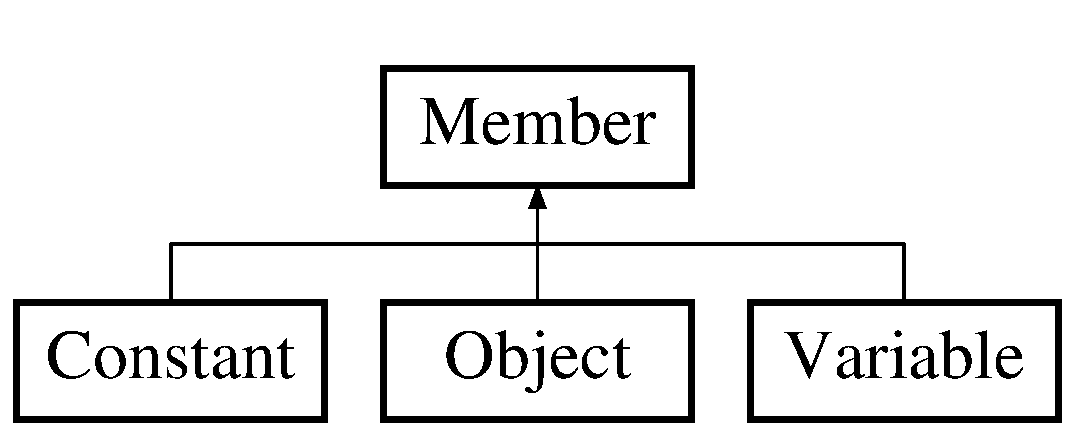
\includegraphics[height=2.000000cm]{classMember}
\end{center}
\end{figure}
\subsection*{Public Member Functions}
\begin{DoxyCompactItemize}
\item 
\hypertarget{classMember_a44241aa6aa9b792b550d9cc29e7ad050}{\hyperlink{classMember_a44241aa6aa9b792b550d9cc29e7ad050}{Member} ()}\label{classMember_a44241aa6aa9b792b550d9cc29e7ad050}

\begin{DoxyCompactList}\small\item\em Constructor. \end{DoxyCompactList}\item 
\hyperlink{classMember_a932fbfb630620b979b19f24a4dc34288}{Member} (string name, vector$<$ \hyperlink{classType}{Type} $\ast$ $>$ types)
\begin{DoxyCompactList}\small\item\em Constructor. \end{DoxyCompactList}\item 
\hypertarget{classMember_a4f5d7cb8788247f65f10b5b81be4a4ab}{virtual \hyperlink{classMember_a4f5d7cb8788247f65f10b5b81be4a4ab}{$\sim$\+Member} ()}\label{classMember_a4f5d7cb8788247f65f10b5b81be4a4ab}

\begin{DoxyCompactList}\small\item\em Destructor -\/ virtual. \end{DoxyCompactList}\item 
void \hyperlink{classMember_a1ada18dd2a55fd384173796936fe286a}{change\+Name} (string name)
\begin{DoxyCompactList}\small\item\em Change the name of the member. \end{DoxyCompactList}\item 
string \hyperlink{classMember_acbe6a0cd073a21fb0f1da2cbfb260952}{get\+Name} ()
\begin{DoxyCompactList}\small\item\em Get the name of the member. \end{DoxyCompactList}\item 
vector$<$ \hyperlink{classType}{Type} $\ast$ $>$ $\ast$ \hyperlink{classMember_a97087e4d42f7a4e5c0d0818748ebb614}{get\+Types} ()
\begin{DoxyCompactList}\small\item\em Get the either type of the member. \end{DoxyCompactList}\item 
virtual string \hyperlink{classMember_aaa0028059dd87706188ee670bd28e4f2}{to\+\_\+string} ()
\begin{DoxyCompactList}\small\item\em Return a string that represent the member -\/ virtual. \end{DoxyCompactList}\item 
virtual string \hyperlink{classMember_a7178ead1b2f1daa5fc5f993281ec90a4}{get\+Class} ()
\begin{DoxyCompactList}\small\item\em Return the name of the class -\/ virtual. \end{DoxyCompactList}\end{DoxyCompactItemize}
\subsection*{Protected Attributes}
\begin{DoxyCompactItemize}
\item 
string \hyperlink{classMember_ac5030aba6f6207335cb970941c3a3f58}{m\+\_\+name}
\item 
\hypertarget{classMember_a9c88befc1b0d8f5df4bda265ee129dfb}{vector$<$ \hyperlink{classType}{Type} $\ast$ $>$ {\bfseries m\+\_\+types}}\label{classMember_a9c88befc1b0d8f5df4bda265ee129dfb}

\end{DoxyCompactItemize}


\subsection{Constructor \& Destructor Documentation}
\hypertarget{classMember_a932fbfb630620b979b19f24a4dc34288}{\index{Member@{Member}!Member@{Member}}
\index{Member@{Member}!Member@{Member}}
\subsubsection[{Member}]{\setlength{\rightskip}{0pt plus 5cm}Member\+::\+Member (
\begin{DoxyParamCaption}
\item[{string}]{name, }
\item[{vector$<$ {\bf Type} $\ast$ $>$}]{types}
\end{DoxyParamCaption}
)}}\label{classMember_a932fbfb630620b979b19f24a4dc34288}


Constructor. 


\begin{DoxyParams}{Parameters}
{\em name} & -\/ name of the member types -\/ either type of the member \\
\hline
\end{DoxyParams}


\subsection{Member Function Documentation}
\hypertarget{classMember_a1ada18dd2a55fd384173796936fe286a}{\index{Member@{Member}!change\+Name@{change\+Name}}
\index{change\+Name@{change\+Name}!Member@{Member}}
\subsubsection[{change\+Name}]{\setlength{\rightskip}{0pt plus 5cm}void Member\+::change\+Name (
\begin{DoxyParamCaption}
\item[{string}]{name}
\end{DoxyParamCaption}
)}}\label{classMember_a1ada18dd2a55fd384173796936fe286a}


Change the name of the member. 


\begin{DoxyParams}{Parameters}
{\em name} & -\/ new name of the member \\
\hline
\end{DoxyParams}
\hypertarget{classMember_a7178ead1b2f1daa5fc5f993281ec90a4}{\index{Member@{Member}!get\+Class@{get\+Class}}
\index{get\+Class@{get\+Class}!Member@{Member}}
\subsubsection[{get\+Class}]{\setlength{\rightskip}{0pt plus 5cm}string Member\+::get\+Class (
\begin{DoxyParamCaption}
{}
\end{DoxyParamCaption}
)\hspace{0.3cm}{\ttfamily [virtual]}}}\label{classMember_a7178ead1b2f1daa5fc5f993281ec90a4}


Return the name of the class -\/ virtual. 

\begin{DoxyReturn}{Returns}
\char`\"{}\+Member\char`\"{} 
\end{DoxyReturn}


Reimplemented in \hyperlink{classConstant_aeb11c90406eb42af86ba8898fb774e1d}{Constant}, \hyperlink{classObject_a397dca51f83eef1e5fc827aed391c2cf}{Object}, and \hyperlink{classVariable_aaebc8ef1594f951323e33725abfd69b5}{Variable}.

\hypertarget{classMember_acbe6a0cd073a21fb0f1da2cbfb260952}{\index{Member@{Member}!get\+Name@{get\+Name}}
\index{get\+Name@{get\+Name}!Member@{Member}}
\subsubsection[{get\+Name}]{\setlength{\rightskip}{0pt plus 5cm}string Member\+::get\+Name (
\begin{DoxyParamCaption}
{}
\end{DoxyParamCaption}
)}}\label{classMember_acbe6a0cd073a21fb0f1da2cbfb260952}


Get the name of the member. 

\begin{DoxyReturn}{Returns}
the string of its name 
\end{DoxyReturn}
\hypertarget{classMember_a97087e4d42f7a4e5c0d0818748ebb614}{\index{Member@{Member}!get\+Types@{get\+Types}}
\index{get\+Types@{get\+Types}!Member@{Member}}
\subsubsection[{get\+Types}]{\setlength{\rightskip}{0pt plus 5cm}vector$<$ {\bf Type} $\ast$ $>$ $\ast$ Member\+::get\+Types (
\begin{DoxyParamCaption}
{}
\end{DoxyParamCaption}
)}}\label{classMember_a97087e4d42f7a4e5c0d0818748ebb614}


Get the either type of the member. 

\begin{DoxyReturn}{Returns}
a pointer to its either type 
\end{DoxyReturn}
\hypertarget{classMember_aaa0028059dd87706188ee670bd28e4f2}{\index{Member@{Member}!to\+\_\+string@{to\+\_\+string}}
\index{to\+\_\+string@{to\+\_\+string}!Member@{Member}}
\subsubsection[{to\+\_\+string}]{\setlength{\rightskip}{0pt plus 5cm}string Member\+::to\+\_\+string (
\begin{DoxyParamCaption}
{}
\end{DoxyParamCaption}
)\hspace{0.3cm}{\ttfamily [virtual]}}}\label{classMember_aaa0028059dd87706188ee670bd28e4f2}


Return a string that represent the member -\/ virtual. 

\begin{DoxyReturn}{Returns}
a string \char`\"{}\+Member name -\/ either type\char`\"{} 
\end{DoxyReturn}


Reimplemented in \hyperlink{classConstant_a685a4dbdc864e61c3e14a0fd974ba024}{Constant}, \hyperlink{classObject_a520e44ab90b2d66a2c5c0874e19a688d}{Object}, and \hyperlink{classVariable_a193be8605a472ddcceba928e746ffac2}{Variable}.



\subsection{Member Data Documentation}
\hypertarget{classMember_ac5030aba6f6207335cb970941c3a3f58}{\index{Member@{Member}!m\+\_\+name@{m\+\_\+name}}
\index{m\+\_\+name@{m\+\_\+name}!Member@{Member}}
\subsubsection[{m\+\_\+name}]{\setlength{\rightskip}{0pt plus 5cm}string Member\+::m\+\_\+name\hspace{0.3cm}{\ttfamily [protected]}}}\label{classMember_ac5030aba6f6207335cb970941c3a3f58}
$<$ name of the member either type of the member 

The documentation for this class was generated from the following files\+:\begin{DoxyCompactItemize}
\item 
src/\hyperlink{member_8h}{member.\+h}\item 
src/\hyperlink{member_8cpp}{member.\+cpp}\end{DoxyCompactItemize}

\hypertarget{classObject}{\section{Object Class Reference}
\label{classObject}\index{Object@{Object}}
}
Inheritance diagram for Object\+:\begin{figure}[H]
\begin{center}
\leavevmode
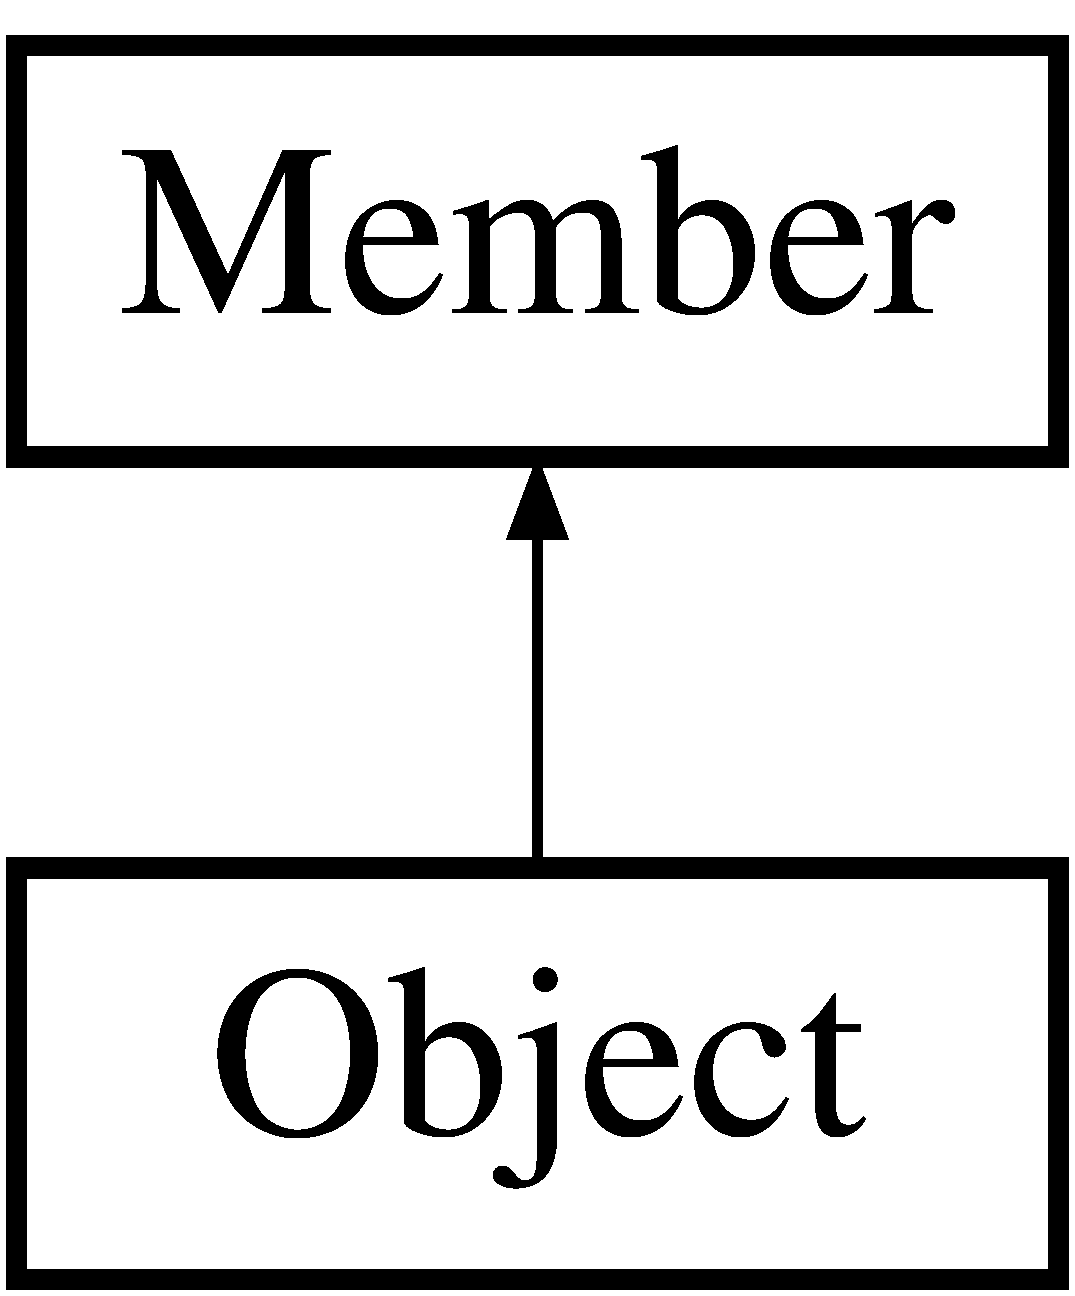
\includegraphics[height=2.000000cm]{classObject}
\end{center}
\end{figure}
\subsection*{Public Member Functions}
\begin{DoxyCompactItemize}
\item 
\hypertarget{classObject_a40860402e64d8008fb42329df7097cdb}{\hyperlink{classObject_a40860402e64d8008fb42329df7097cdb}{Object} ()}\label{classObject_a40860402e64d8008fb42329df7097cdb}

\begin{DoxyCompactList}\small\item\em Constructor. \end{DoxyCompactList}\item 
\hyperlink{classObject_af8967f65b73ffa66578b53f35521a926}{Object} (string name, vector$<$ \hyperlink{classType}{Type} $\ast$ $>$ types)
\begin{DoxyCompactList}\small\item\em Constructor. \end{DoxyCompactList}\item 
void \hyperlink{classObject_a8b4ff24815dcc0704db8db212b2ed01f}{add\+Types} (vector$<$ \hyperlink{classType}{Type} $\ast$ $>$ types)
\begin{DoxyCompactList}\small\item\em Add an either type to the existing either type of the object (doesn't duplicate) \end{DoxyCompactList}\item 
string \hyperlink{classObject_a520e44ab90b2d66a2c5c0874e19a688d}{to\+\_\+string} ()
\begin{DoxyCompactList}\small\item\em Return a string that represent the object. \end{DoxyCompactList}\item 
string \hyperlink{classObject_a397dca51f83eef1e5fc827aed391c2cf}{get\+Class} ()
\begin{DoxyCompactList}\small\item\em Return the name of the class. \end{DoxyCompactList}\end{DoxyCompactItemize}
\subsection*{Additional Inherited Members}


\subsection{Constructor \& Destructor Documentation}
\hypertarget{classObject_af8967f65b73ffa66578b53f35521a926}{\index{Object@{Object}!Object@{Object}}
\index{Object@{Object}!Object@{Object}}
\subsubsection[{Object}]{\setlength{\rightskip}{0pt plus 5cm}Object\+::\+Object (
\begin{DoxyParamCaption}
\item[{string}]{name, }
\item[{vector$<$ {\bf Type} $\ast$ $>$}]{types}
\end{DoxyParamCaption}
)}}\label{classObject_af8967f65b73ffa66578b53f35521a926}


Constructor. 


\begin{DoxyParams}{Parameters}
{\em name} & -\/ name of the object types -\/ either type of the object \\
\hline
\end{DoxyParams}


\subsection{Member Function Documentation}
\hypertarget{classObject_a8b4ff24815dcc0704db8db212b2ed01f}{\index{Object@{Object}!add\+Types@{add\+Types}}
\index{add\+Types@{add\+Types}!Object@{Object}}
\subsubsection[{add\+Types}]{\setlength{\rightskip}{0pt plus 5cm}void Object\+::add\+Types (
\begin{DoxyParamCaption}
\item[{vector$<$ {\bf Type} $\ast$ $>$}]{types}
\end{DoxyParamCaption}
)}}\label{classObject_a8b4ff24815dcc0704db8db212b2ed01f}


Add an either type to the existing either type of the object (doesn't duplicate) 


\begin{DoxyParams}{Parameters}
{\em types} & -\/ either type to add to the object \\
\hline
\end{DoxyParams}
\hypertarget{classObject_a397dca51f83eef1e5fc827aed391c2cf}{\index{Object@{Object}!get\+Class@{get\+Class}}
\index{get\+Class@{get\+Class}!Object@{Object}}
\subsubsection[{get\+Class}]{\setlength{\rightskip}{0pt plus 5cm}string Object\+::get\+Class (
\begin{DoxyParamCaption}
{}
\end{DoxyParamCaption}
)\hspace{0.3cm}{\ttfamily [virtual]}}}\label{classObject_a397dca51f83eef1e5fc827aed391c2cf}


Return the name of the class. 

\begin{DoxyReturn}{Returns}
\char`\"{}\+Object\char`\"{} 
\end{DoxyReturn}


Reimplemented from \hyperlink{classMember_a7178ead1b2f1daa5fc5f993281ec90a4}{Member}.

\hypertarget{classObject_a520e44ab90b2d66a2c5c0874e19a688d}{\index{Object@{Object}!to\+\_\+string@{to\+\_\+string}}
\index{to\+\_\+string@{to\+\_\+string}!Object@{Object}}
\subsubsection[{to\+\_\+string}]{\setlength{\rightskip}{0pt plus 5cm}string Object\+::to\+\_\+string (
\begin{DoxyParamCaption}
{}
\end{DoxyParamCaption}
)\hspace{0.3cm}{\ttfamily [virtual]}}}\label{classObject_a520e44ab90b2d66a2c5c0874e19a688d}


Return a string that represent the object. 

\begin{DoxyReturn}{Returns}
a string \char`\"{}\+Object name -\/ either type\char`\"{} 
\end{DoxyReturn}


Reimplemented from \hyperlink{classMember_aaa0028059dd87706188ee670bd28e4f2}{Member}.



The documentation for this class was generated from the following files\+:\begin{DoxyCompactItemize}
\item 
src/\hyperlink{object_8h}{object.\+h}\item 
src/object.\+cpp\end{DoxyCompactItemize}

\hypertarget{classParser}{\section{Parser Class Reference}
\label{classParser}\index{Parser@{Parser}}
}
Inheritance diagram for Parser\+:\begin{figure}[H]
\begin{center}
\leavevmode
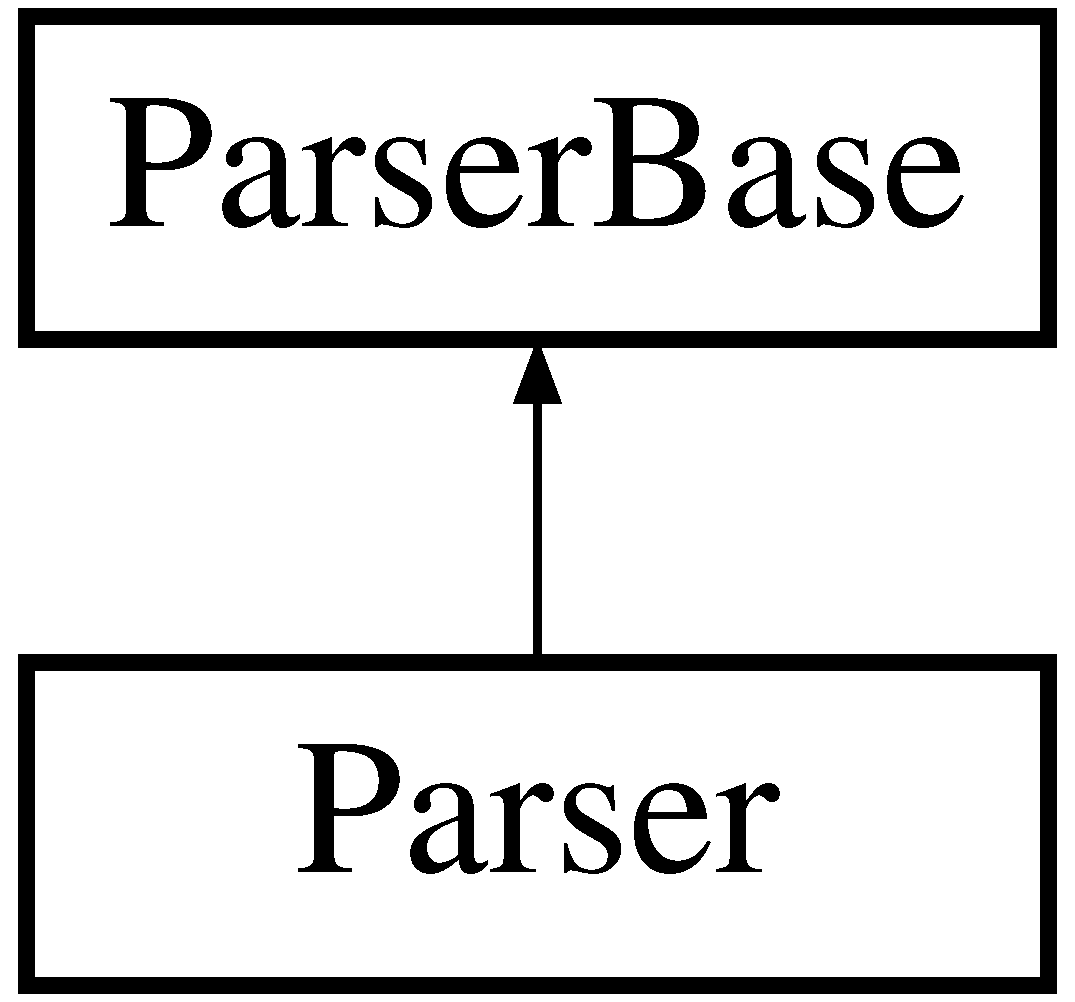
\includegraphics[height=2.000000cm]{classParser}
\end{center}
\end{figure}
\subsection*{Public Member Functions}
\begin{DoxyCompactItemize}
\item 
int \hyperlink{classParser_af677db3c393c6b50d839290ad1af7d1d}{parse} ()
\begin{DoxyCompactList}\small\item\em Parsing function. \end{DoxyCompactList}\item 
\hypertarget{classParser_abdc68932f658c4a203aa97ab368f0d2b}{void \hyperlink{classParser_abdc68932f658c4a203aa97ab368f0d2b}{init} ()}\label{classParser_abdc68932f658c4a203aa97ab368f0d2b}

\begin{DoxyCompactList}\small\item\em Init the data. \end{DoxyCompactList}\item 
void \hyperlink{classParser_a280a5db9d433fd9a5d90aed3ec240a41}{set\+Data} (\hyperlink{classParser}{Parser} $\ast$parser)
\begin{DoxyCompactList}\small\item\em Copy the data of another \hyperlink{classParser}{Parser} in order to parse another file (used to parse the problem file after having parsed the domain file) \end{DoxyCompactList}\item 
\hyperlink{classData}{Data} $\ast$ \hyperlink{classParser_a6202bf4573fd50d5e052640177ca2289}{get\+Data} ()
\begin{DoxyCompactList}\small\item\em Get the pointer to the data. \end{DoxyCompactList}\item 
void \hyperlink{classParser_abd319a3d809d96b35da0b07160080ff1}{add\+Domain} (std\+::string $\ast$name)
\begin{DoxyCompactList}\small\item\em Set the name of the domain. \end{DoxyCompactList}\item 
bool \hyperlink{classParser_ae97c849415a4b6943b45d2e314a89795}{is\+Domain} (std\+::string $\ast$name)
\begin{DoxyCompactList}\small\item\em Verify if name is the name of the domain previously parsed. \end{DoxyCompactList}\item 
bool \hyperlink{classParser_a16caa057293d617e95e374ec3101c023}{add\+Requirement} (int req)
\begin{DoxyCompactList}\small\item\em Add the requirement req once read in \+:requirements. \end{DoxyCompactList}\item 
bool \hyperlink{classParser_a2963392154c748d42f9050700d28f1b3}{is\+Requirement} (int req)
\begin{DoxyCompactList}\small\item\em Verify if the requirement req has been announced in \+:requirements. \end{DoxyCompactList}\item 
bool \hyperlink{classParser_af729ba7522ed318d4815c05d220cf3f2}{add\+Types} (std\+::vector$<$ \hyperlink{classTypedList}{Typed\+List} $\ast$ $>$ $\ast$typed\+List\+\_\+list)
\begin{DoxyCompactList}\small\item\em Add the types once read in \+:types. \end{DoxyCompactList}\item 
bool \hyperlink{classParser_a8a0cab70a42a5864b1c88e52ea67bdbc}{add\+Constants} (std\+::vector$<$ \hyperlink{classTypedList}{Typed\+List} $\ast$ $>$ $\ast$typed\+List\+\_\+list)
\begin{DoxyCompactList}\small\item\em Add the constants once read in \+:constants. \end{DoxyCompactList}\item 
bool \hyperlink{classParser_a2bb6e04284ea6e2169672c6de405f665}{add\+Predicate} (std\+::string $\ast$name, std\+::vector$<$ \hyperlink{classTypedList}{Typed\+List} $\ast$ $>$ $\ast$typed\+List\+\_\+list)
\begin{DoxyCompactList}\small\item\em Add the predicates once read in \+:predicates. \end{DoxyCompactList}\item 
bool \hyperlink{classParser_ac19e3969c2c41180cf1ed2e9e99a780a}{add\+Functions} (std\+::vector$<$ std\+::pair$<$ std\+::string $\ast$, std\+::vector$<$ \hyperlink{classTypedList}{Typed\+List} $\ast$ $>$ $\ast$ $>$ $\ast$ $>$ $\ast$function\+\_\+skeleton\+\_\+list, std\+::vector$<$ std\+::string $>$ $\ast$return\+\_\+type)
\begin{DoxyCompactList}\small\item\em Add the functions once read in \+:functions. \end{DoxyCompactList}\item 
bool \hyperlink{classParser_ac9d6477dcb6f8d7b6995f9b1b35c5805}{add\+Durative\+Action} (std\+::string $\ast$name, std\+::vector$<$ \hyperlink{classTypedList}{Typed\+List} $\ast$ $>$ $\ast$typed\+List\+\_\+list, float number, std\+::vector$<$ std\+::pair$<$ std\+::pair$<$ std\+::vector$<$ std\+::string $>$ $\ast$, std\+::string $\ast$ $>$ $\ast$, int $>$ $\ast$ $>$ $\ast$timed\+\_\+\+G\+D, std\+::vector$<$ std\+::pair$<$ std\+::pair$<$ std\+::vector$<$ std\+::string $>$ $\ast$, std\+::string $\ast$ $>$ $\ast$, int $>$ $\ast$ $>$ $\ast$cond\+\_\+effect)
\begin{DoxyCompactList}\small\item\em Add adurative-\/action once read in \+:durative-\/action. \end{DoxyCompactList}\item 
void \hyperlink{classParser_a40779a6e2c720a1415a0c824bf079b47}{add\+Problem} (std\+::string $\ast$name)
\begin{DoxyCompactList}\small\item\em Set the name of the problem. \end{DoxyCompactList}\item 
bool \hyperlink{classParser_a5784fcd1e2de901d7a0f12412754b724}{add\+Objects} (std\+::vector$<$ \hyperlink{classTypedList}{Typed\+List} $\ast$ $>$ $\ast$typed\+List\+\_\+list)
\begin{DoxyCompactList}\small\item\em Add the objects once read in \+:objects and add the name of this object in m\+\_\+object\+\_\+list. \end{DoxyCompactList}\item 
bool \hyperlink{classParser_aaae009ea97709247577c76937427ffef}{add\+Init} (std\+::pair$<$ std\+::pair$<$ std\+::vector$<$ std\+::string $>$ $\ast$, std\+::string $\ast$ $>$ $\ast$, bool $>$ $\ast$literal, float at)
\begin{DoxyCompactList}\small\item\em Add an init fluent once read in \+:init. \end{DoxyCompactList}\item 
bool \hyperlink{classParser_ac7b9f22b8589d44b28ad5170f1b9b403}{add\+Goals} (std\+::vector$<$ std\+::vector$<$ std\+::pair$<$ std\+::pair$<$ std\+::vector$<$ std\+::string $>$ $\ast$, std\+::string $\ast$ $>$ $\ast$, int $>$ $\ast$ $>$ $\ast$ $>$ $\ast$pre\+\_\+\+G\+D)
\begin{DoxyCompactList}\small\item\em Add the goal fluents once read in \+:goal. \end{DoxyCompactList}\item 
bool \hyperlink{classParser_ab243bf4f6ec47e9c10c42509d0ed14ec}{add\+Initiated\+Function} (std\+::pair$<$ std\+::vector$<$ std\+::string $>$ $\ast$, std\+::string $\ast$ $>$ $\ast$atomic\+\_\+formula, float number)
\begin{DoxyCompactList}\small\item\em Add an initiated function once read in \+:init. \end{DoxyCompactList}\item 
\hypertarget{classParser_a90540c5d1f12d7a5974efdf526fb6d22}{void \hyperlink{classParser_a90540c5d1f12d7a5974efdf526fb6d22}{display} ()}\label{classParser_a90540c5d1f12d7a5974efdf526fb6d22}

\begin{DoxyCompactList}\small\item\em Display the data (domain variables, problem variables, and errors) in stdout. \end{DoxyCompactList}\item 
void \hyperlink{classParser_ab2075cf762895993dc7583855350203b}{lexical\+\_\+error} (std\+::string msg)
\begin{DoxyCompactList}\small\item\em Add a warning. \end{DoxyCompactList}\item 
void \hyperlink{classParser_a1dd4f26466b3b3e51046cd8dfa085a4f}{fatal\+\_\+error} (std\+::string msg)
\begin{DoxyCompactList}\small\item\em Stop the execution and print the error message on stderr. \end{DoxyCompactList}\item 
float \hyperlink{classParser_acdaf00eb98e4f6fe1b834bc23173566c}{get\+Function\+Return} (std\+::string $\ast$name, std\+::vector$<$ std\+::string $>$ $\ast$list\+\_\+term)
\begin{DoxyCompactList}\small\item\em Get the return of an initiated function. \end{DoxyCompactList}\end{DoxyCompactItemize}
\subsection*{Additional Inherited Members}


\subsection{Member Function Documentation}
\hypertarget{classParser_a8a0cab70a42a5864b1c88e52ea67bdbc}{\index{Parser@{Parser}!add\+Constants@{add\+Constants}}
\index{add\+Constants@{add\+Constants}!Parser@{Parser}}
\subsubsection[{add\+Constants}]{\setlength{\rightskip}{0pt plus 5cm}bool Parser\+::add\+Constants (
\begin{DoxyParamCaption}
\item[{std\+::vector$<$ {\bf Typed\+List} $\ast$ $>$ $\ast$}]{typed\+List\+\_\+list}
\end{DoxyParamCaption}
)\hspace{0.3cm}{\ttfamily [inline]}}}\label{classParser_a8a0cab70a42a5864b1c88e52ea67bdbc}


Add the constants once read in \+:constants. 


\begin{DoxyParams}{Parameters}
{\em typed\+List\+\_\+list} & -\/ list of constants \+: (constants\+List, types\+List) \\
\hline
\end{DoxyParams}
\begin{DoxyReturn}{Returns}
false something went wrong 
\end{DoxyReturn}
\hypertarget{classParser_abd319a3d809d96b35da0b07160080ff1}{\index{Parser@{Parser}!add\+Domain@{add\+Domain}}
\index{add\+Domain@{add\+Domain}!Parser@{Parser}}
\subsubsection[{add\+Domain}]{\setlength{\rightskip}{0pt plus 5cm}void Parser\+::add\+Domain (
\begin{DoxyParamCaption}
\item[{std\+::string $\ast$}]{name}
\end{DoxyParamCaption}
)\hspace{0.3cm}{\ttfamily [inline]}}}\label{classParser_abd319a3d809d96b35da0b07160080ff1}


Set the name of the domain. 


\begin{DoxyParams}{Parameters}
{\em name} & -\/ name of the domain \\
\hline
\end{DoxyParams}
\hypertarget{classParser_ac9d6477dcb6f8d7b6995f9b1b35c5805}{\index{Parser@{Parser}!add\+Durative\+Action@{add\+Durative\+Action}}
\index{add\+Durative\+Action@{add\+Durative\+Action}!Parser@{Parser}}
\subsubsection[{add\+Durative\+Action}]{\setlength{\rightskip}{0pt plus 5cm}bool Parser\+::add\+Durative\+Action (
\begin{DoxyParamCaption}
\item[{std\+::string $\ast$}]{name, }
\item[{std\+::vector$<$ {\bf Typed\+List} $\ast$ $>$ $\ast$}]{typed\+List\+\_\+list, }
\item[{float}]{number, }
\item[{std\+::vector$<$ std\+::pair$<$ std\+::pair$<$ std\+::vector$<$ std\+::string $>$ $\ast$, std\+::string $\ast$ $>$ $\ast$, int $>$ $\ast$ $>$ $\ast$}]{timed\+\_\+\+G\+D, }
\item[{std\+::vector$<$ std\+::pair$<$ std\+::pair$<$ std\+::vector$<$ std\+::string $>$ $\ast$, std\+::string $\ast$ $>$ $\ast$, int $>$ $\ast$ $>$ $\ast$}]{cond\+\_\+effect}
\end{DoxyParamCaption}
)\hspace{0.3cm}{\ttfamily [inline]}}}\label{classParser_ac9d6477dcb6f8d7b6995f9b1b35c5805}


Add adurative-\/action once read in \+:durative-\/action. 


\begin{DoxyParams}{Parameters}
{\em name} & -\/ name of the durative-\/action typed\+List\+\_\+list -\/ parameters (variables) of the durative-\/action \+: (variables\+List, types\+List) timed\+\_\+\+G\+D -\/ preconditions of the durative-\/action \+: list(pair(pair(fluent\+Parameters, fluent\+Name), prec\+Type)) cond\+\_\+effect -\/ effects of the durative-\/action \+: list(pair(pair(fluent\+Parameters, fluent\+Name), effect\+Type)) \\
\hline
\end{DoxyParams}
\begin{DoxyReturn}{Returns}
false something went wrong, such as a predicate that hasn't been defined 
\end{DoxyReturn}
\hypertarget{classParser_ac19e3969c2c41180cf1ed2e9e99a780a}{\index{Parser@{Parser}!add\+Functions@{add\+Functions}}
\index{add\+Functions@{add\+Functions}!Parser@{Parser}}
\subsubsection[{add\+Functions}]{\setlength{\rightskip}{0pt plus 5cm}bool Parser\+::add\+Functions (
\begin{DoxyParamCaption}
\item[{std\+::vector$<$ std\+::pair$<$ std\+::string $\ast$, std\+::vector$<$ {\bf Typed\+List} $\ast$ $>$ $\ast$ $>$ $\ast$ $>$ $\ast$}]{function\+\_\+skeleton\+\_\+list, }
\item[{std\+::vector$<$ std\+::string $>$ $\ast$}]{return\+\_\+type}
\end{DoxyParamCaption}
)\hspace{0.3cm}{\ttfamily [inline]}}}\label{classParser_ac19e3969c2c41180cf1ed2e9e99a780a}


Add the functions once read in \+:functions. 


\begin{DoxyParams}{Parameters}
{\em function\+\_\+skeleton\+\_\+list} & -\/ list of the functions' pairs of name and parameters return\+\_\+type -\/ the type of the return (list for either representation) \\
\hline
\end{DoxyParams}
\begin{DoxyReturn}{Returns}
false something went wrong 
\end{DoxyReturn}
\hypertarget{classParser_ac7b9f22b8589d44b28ad5170f1b9b403}{\index{Parser@{Parser}!add\+Goals@{add\+Goals}}
\index{add\+Goals@{add\+Goals}!Parser@{Parser}}
\subsubsection[{add\+Goals}]{\setlength{\rightskip}{0pt plus 5cm}bool Parser\+::add\+Goals (
\begin{DoxyParamCaption}
\item[{std\+::vector$<$ std\+::vector$<$ std\+::pair$<$ std\+::pair$<$ std\+::vector$<$ std\+::string $>$ $\ast$, std\+::string $\ast$ $>$ $\ast$, int $>$ $\ast$ $>$ $\ast$ $>$ $\ast$}]{pre\+\_\+\+G\+D}
\end{DoxyParamCaption}
)\hspace{0.3cm}{\ttfamily [inline]}}}\label{classParser_ac7b9f22b8589d44b28ad5170f1b9b403}


Add the goal fluents once read in \+:goal. 


\begin{DoxyParams}{Parameters}
{\em pre\+\_\+\+G\+D} & -\/ list of fluents () \\
\hline
\end{DoxyParams}
\begin{DoxyReturn}{Returns}
false something went wrong, such as a fluent of which the predicate hasn't been defined 
\end{DoxyReturn}
\hypertarget{classParser_aaae009ea97709247577c76937427ffef}{\index{Parser@{Parser}!add\+Init@{add\+Init}}
\index{add\+Init@{add\+Init}!Parser@{Parser}}
\subsubsection[{add\+Init}]{\setlength{\rightskip}{0pt plus 5cm}bool Parser\+::add\+Init (
\begin{DoxyParamCaption}
\item[{std\+::pair$<$ std\+::pair$<$ std\+::vector$<$ std\+::string $>$ $\ast$, std\+::string $\ast$ $>$ $\ast$, bool $>$ $\ast$}]{literal, }
\item[{float}]{at}
\end{DoxyParamCaption}
)\hspace{0.3cm}{\ttfamily [inline]}}}\label{classParser_aaae009ea97709247577c76937427ffef}


Add an init fluent once read in \+:init. 


\begin{DoxyParams}{Parameters}
{\em literal} & -\/ fluent \+: pair(pair(parameters, name), positive) at -\/ time when this init is effctive \\
\hline
\end{DoxyParams}
\begin{DoxyReturn}{Returns}
false something went wrong, such as a fluent of which the predicate hasn't been defined 
\end{DoxyReturn}
\hypertarget{classParser_ab243bf4f6ec47e9c10c42509d0ed14ec}{\index{Parser@{Parser}!add\+Initiated\+Function@{add\+Initiated\+Function}}
\index{add\+Initiated\+Function@{add\+Initiated\+Function}!Parser@{Parser}}
\subsubsection[{add\+Initiated\+Function}]{\setlength{\rightskip}{0pt plus 5cm}bool Parser\+::add\+Initiated\+Function (
\begin{DoxyParamCaption}
\item[{std\+::pair$<$ std\+::vector$<$ std\+::string $>$ $\ast$, std\+::string $\ast$ $>$ $\ast$}]{atomic\+\_\+formula, }
\item[{float}]{number}
\end{DoxyParamCaption}
)\hspace{0.3cm}{\ttfamily [inline]}}}\label{classParser_ab243bf4f6ec47e9c10c42509d0ed14ec}


Add an initiated function once read in \+:init. 


\begin{DoxyParams}{Parameters}
{\em atomic\+\_\+formula} & -\/ name and parameters \+: pair(parameters, name) number -\/ the return of the initiated function \\
\hline
\end{DoxyParams}
\begin{DoxyReturn}{Returns}
false something went wrong, such as a function or an object or a constant that hasn't been defined 
\end{DoxyReturn}
\hypertarget{classParser_a5784fcd1e2de901d7a0f12412754b724}{\index{Parser@{Parser}!add\+Objects@{add\+Objects}}
\index{add\+Objects@{add\+Objects}!Parser@{Parser}}
\subsubsection[{add\+Objects}]{\setlength{\rightskip}{0pt plus 5cm}bool Parser\+::add\+Objects (
\begin{DoxyParamCaption}
\item[{std\+::vector$<$ {\bf Typed\+List} $\ast$ $>$ $\ast$}]{typed\+List\+\_\+list}
\end{DoxyParamCaption}
)\hspace{0.3cm}{\ttfamily [inline]}}}\label{classParser_a5784fcd1e2de901d7a0f12412754b724}


Add the objects once read in \+:objects and add the name of this object in m\+\_\+object\+\_\+list. 


\begin{DoxyParams}{Parameters}
{\em typed\+List\+\_\+list} & -\/ list of objects \+: (objects\+List, types\+List) \\
\hline
\end{DoxyParams}
\begin{DoxyReturn}{Returns}
false something went wrong 
\end{DoxyReturn}
\hypertarget{classParser_a2bb6e04284ea6e2169672c6de405f665}{\index{Parser@{Parser}!add\+Predicate@{add\+Predicate}}
\index{add\+Predicate@{add\+Predicate}!Parser@{Parser}}
\subsubsection[{add\+Predicate}]{\setlength{\rightskip}{0pt plus 5cm}bool Parser\+::add\+Predicate (
\begin{DoxyParamCaption}
\item[{std\+::string $\ast$}]{name, }
\item[{std\+::vector$<$ {\bf Typed\+List} $\ast$ $>$ $\ast$}]{typed\+List\+\_\+list}
\end{DoxyParamCaption}
)\hspace{0.3cm}{\ttfamily [inline]}}}\label{classParser_a2bb6e04284ea6e2169672c6de405f665}


Add the predicates once read in \+:predicates. 


\begin{DoxyParams}{Parameters}
{\em name} & -\/ the name of the predicate typed\+List\+\_\+list -\/ list of parameters \+: (variables\+List, types\+List) \\
\hline
\end{DoxyParams}
\begin{DoxyReturn}{Returns}
false something went wrong 
\end{DoxyReturn}
\hypertarget{classParser_a40779a6e2c720a1415a0c824bf079b47}{\index{Parser@{Parser}!add\+Problem@{add\+Problem}}
\index{add\+Problem@{add\+Problem}!Parser@{Parser}}
\subsubsection[{add\+Problem}]{\setlength{\rightskip}{0pt plus 5cm}void Parser\+::add\+Problem (
\begin{DoxyParamCaption}
\item[{std\+::string $\ast$}]{name}
\end{DoxyParamCaption}
)\hspace{0.3cm}{\ttfamily [inline]}}}\label{classParser_a40779a6e2c720a1415a0c824bf079b47}


Set the name of the problem. 


\begin{DoxyParams}{Parameters}
{\em name} & -\/ name of the problem \\
\hline
\end{DoxyParams}
\hypertarget{classParser_a16caa057293d617e95e374ec3101c023}{\index{Parser@{Parser}!add\+Requirement@{add\+Requirement}}
\index{add\+Requirement@{add\+Requirement}!Parser@{Parser}}
\subsubsection[{add\+Requirement}]{\setlength{\rightskip}{0pt plus 5cm}bool Parser\+::add\+Requirement (
\begin{DoxyParamCaption}
\item[{int}]{req}
\end{DoxyParamCaption}
)\hspace{0.3cm}{\ttfamily [inline]}}}\label{classParser_a16caa057293d617e95e374ec3101c023}


Add the requirement req once read in \+:requirements. 


\begin{DoxyParams}{Parameters}
{\em req} & -\/ Token of the requirement \\
\hline
\end{DoxyParams}
\begin{DoxyReturn}{Returns}
false if the requirement already exists, else true 
\end{DoxyReturn}
\hypertarget{classParser_af729ba7522ed318d4815c05d220cf3f2}{\index{Parser@{Parser}!add\+Types@{add\+Types}}
\index{add\+Types@{add\+Types}!Parser@{Parser}}
\subsubsection[{add\+Types}]{\setlength{\rightskip}{0pt plus 5cm}bool Parser\+::add\+Types (
\begin{DoxyParamCaption}
\item[{std\+::vector$<$ {\bf Typed\+List} $\ast$ $>$ $\ast$}]{typed\+List\+\_\+list}
\end{DoxyParamCaption}
)\hspace{0.3cm}{\ttfamily [inline]}}}\label{classParser_af729ba7522ed318d4815c05d220cf3f2}


Add the types once read in \+:types. 


\begin{DoxyParams}{Parameters}
{\em typed\+List\+\_\+list} & -\/ list of types \+: (types\+List, parent\+Types\+List) \\
\hline
\end{DoxyParams}
\begin{DoxyReturn}{Returns}
false something went wrong 
\end{DoxyReturn}
\hypertarget{classParser_a1dd4f26466b3b3e51046cd8dfa085a4f}{\index{Parser@{Parser}!fatal\+\_\+error@{fatal\+\_\+error}}
\index{fatal\+\_\+error@{fatal\+\_\+error}!Parser@{Parser}}
\subsubsection[{fatal\+\_\+error}]{\setlength{\rightskip}{0pt plus 5cm}void Parser\+::fatal\+\_\+error (
\begin{DoxyParamCaption}
\item[{std\+::string}]{msg}
\end{DoxyParamCaption}
)\hspace{0.3cm}{\ttfamily [inline]}}}\label{classParser_a1dd4f26466b3b3e51046cd8dfa085a4f}


Stop the execution and print the error message on stderr. 


\begin{DoxyParams}{Parameters}
{\em msg} & -\/ message of the error \\
\hline
\end{DoxyParams}
\hypertarget{classParser_a6202bf4573fd50d5e052640177ca2289}{\index{Parser@{Parser}!get\+Data@{get\+Data}}
\index{get\+Data@{get\+Data}!Parser@{Parser}}
\subsubsection[{get\+Data}]{\setlength{\rightskip}{0pt plus 5cm}{\bf Data}$\ast$ Parser\+::get\+Data (
\begin{DoxyParamCaption}
{}
\end{DoxyParamCaption}
)\hspace{0.3cm}{\ttfamily [inline]}}}\label{classParser_a6202bf4573fd50d5e052640177ca2289}


Get the pointer to the data. 

\begin{DoxyReturn}{Returns}
a pointer to the data 
\end{DoxyReturn}
\hypertarget{classParser_acdaf00eb98e4f6fe1b834bc23173566c}{\index{Parser@{Parser}!get\+Function\+Return@{get\+Function\+Return}}
\index{get\+Function\+Return@{get\+Function\+Return}!Parser@{Parser}}
\subsubsection[{get\+Function\+Return}]{\setlength{\rightskip}{0pt plus 5cm}float Parser\+::get\+Function\+Return (
\begin{DoxyParamCaption}
\item[{std\+::string $\ast$}]{name, }
\item[{std\+::vector$<$ std\+::string $>$ $\ast$}]{list\+\_\+term}
\end{DoxyParamCaption}
)\hspace{0.3cm}{\ttfamily [inline]}}}\label{classParser_acdaf00eb98e4f6fe1b834bc23173566c}


Get the return of an initiated function. 


\begin{DoxyParams}{Parameters}
{\em name} & -\/ the name of the function list\+\_\+term -\/ list of parameters \\
\hline
\end{DoxyParams}
\begin{DoxyReturn}{Returns}
the return of the function, and -\/1.\+0 if the function hasn't been found in m\+\_\+initiated\+\_\+functions 
\end{DoxyReturn}
\hypertarget{classParser_ae97c849415a4b6943b45d2e314a89795}{\index{Parser@{Parser}!is\+Domain@{is\+Domain}}
\index{is\+Domain@{is\+Domain}!Parser@{Parser}}
\subsubsection[{is\+Domain}]{\setlength{\rightskip}{0pt plus 5cm}bool Parser\+::is\+Domain (
\begin{DoxyParamCaption}
\item[{std\+::string $\ast$}]{name}
\end{DoxyParamCaption}
)\hspace{0.3cm}{\ttfamily [inline]}}}\label{classParser_ae97c849415a4b6943b45d2e314a89795}


Verify if name is the name of the domain previously parsed. 


\begin{DoxyParams}{Parameters}
{\em name} & -\/ name of the domain of the problem \\
\hline
\end{DoxyParams}
\hypertarget{classParser_a2963392154c748d42f9050700d28f1b3}{\index{Parser@{Parser}!is\+Requirement@{is\+Requirement}}
\index{is\+Requirement@{is\+Requirement}!Parser@{Parser}}
\subsubsection[{is\+Requirement}]{\setlength{\rightskip}{0pt plus 5cm}bool Parser\+::is\+Requirement (
\begin{DoxyParamCaption}
\item[{int}]{req}
\end{DoxyParamCaption}
)\hspace{0.3cm}{\ttfamily [inline]}}}\label{classParser_a2963392154c748d42f9050700d28f1b3}


Verify if the requirement req has been announced in \+:requirements. 


\begin{DoxyParams}{Parameters}
{\em req} & -\/ Token of the requirement \\
\hline
\end{DoxyParams}
\hypertarget{classParser_ab2075cf762895993dc7583855350203b}{\index{Parser@{Parser}!lexical\+\_\+error@{lexical\+\_\+error}}
\index{lexical\+\_\+error@{lexical\+\_\+error}!Parser@{Parser}}
\subsubsection[{lexical\+\_\+error}]{\setlength{\rightskip}{0pt plus 5cm}void Parser\+::lexical\+\_\+error (
\begin{DoxyParamCaption}
\item[{std\+::string}]{msg}
\end{DoxyParamCaption}
)\hspace{0.3cm}{\ttfamily [inline]}}}\label{classParser_ab2075cf762895993dc7583855350203b}


Add a warning. 


\begin{DoxyParams}{Parameters}
{\em msg} & -\/ message of the error \\
\hline
\end{DoxyParams}
\hypertarget{classParser_af677db3c393c6b50d839290ad1af7d1d}{\index{Parser@{Parser}!parse@{parse}}
\index{parse@{parse}!Parser@{Parser}}
\subsubsection[{parse}]{\setlength{\rightskip}{0pt plus 5cm}int Parser\+::parse (
\begin{DoxyParamCaption}
{}
\end{DoxyParamCaption}
)}}\label{classParser_af677db3c393c6b50d839290ad1af7d1d}


Parsing function. 

\begin{DoxyReturn}{Returns}
0 if nothing went wrong 
\end{DoxyReturn}
\hypertarget{classParser_a280a5db9d433fd9a5d90aed3ec240a41}{\index{Parser@{Parser}!set\+Data@{set\+Data}}
\index{set\+Data@{set\+Data}!Parser@{Parser}}
\subsubsection[{set\+Data}]{\setlength{\rightskip}{0pt plus 5cm}void Parser\+::set\+Data (
\begin{DoxyParamCaption}
\item[{{\bf Parser} $\ast$}]{parser}
\end{DoxyParamCaption}
)\hspace{0.3cm}{\ttfamily [inline]}}}\label{classParser_a280a5db9d433fd9a5d90aed3ec240a41}


Copy the data of another \hyperlink{classParser}{Parser} in order to parse another file (used to parse the problem file after having parsed the domain file) 


\begin{DoxyParams}{Parameters}
{\em parser} & -\/ the \hyperlink{classParser}{Parser} object that contains the data to copy \\
\hline
\end{DoxyParams}


The documentation for this class was generated from the following files\+:\begin{DoxyCompactItemize}
\item 
parser/\hyperlink{Parser_8h}{Parser.\+h}\item 
parser/parse.\+cc\end{DoxyCompactItemize}

\hypertarget{classParserBase}{\section{Parser\+Base Class Reference}
\label{classParserBase}\index{Parser\+Base@{Parser\+Base}}
}
Inheritance diagram for Parser\+Base\+:\begin{figure}[H]
\begin{center}
\leavevmode
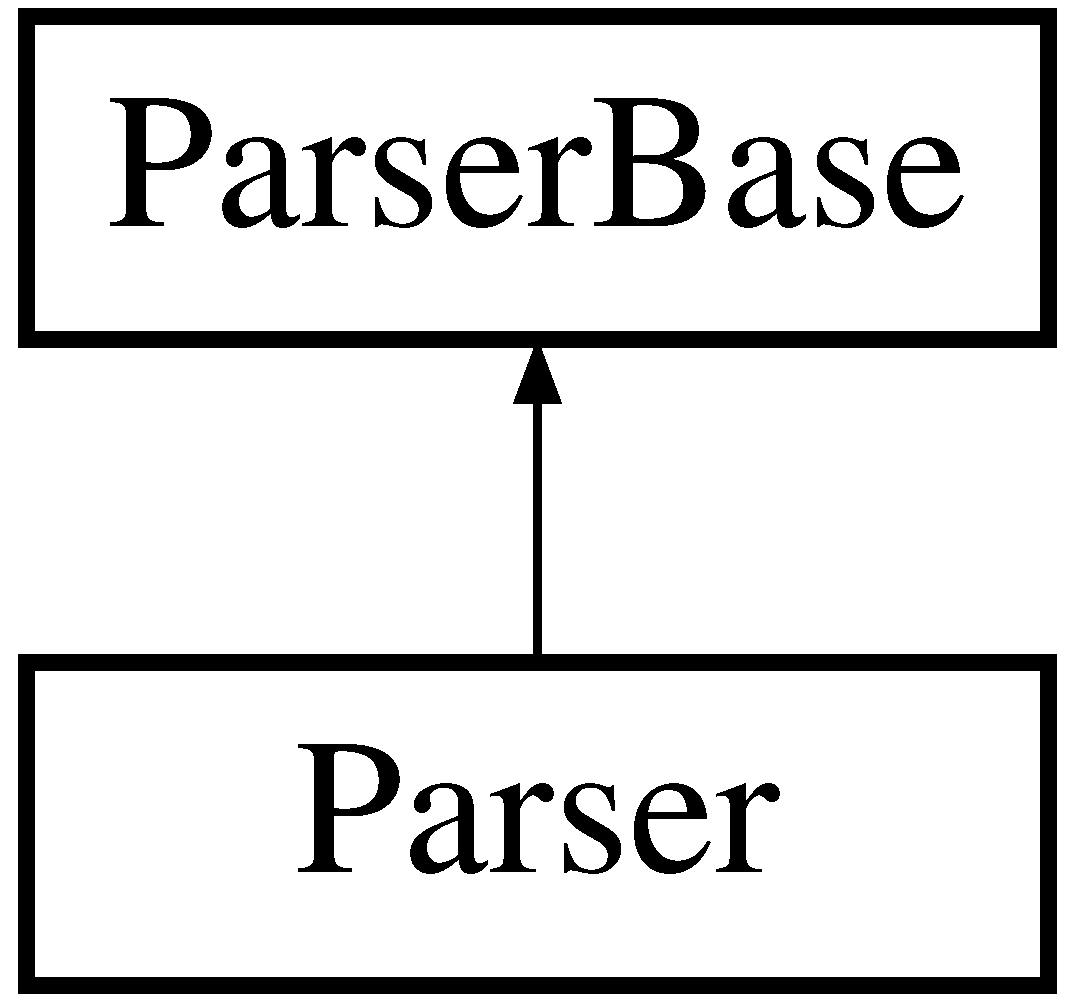
\includegraphics[height=2.000000cm]{classParserBase}
\end{center}
\end{figure}
\subsection*{Classes}
\begin{DoxyCompactItemize}
\item 
union \hyperlink{unionParserBase_1_1STYPE____}{S\+T\+Y\+P\+E\+\_\+\+\_\+}
\end{DoxyCompactItemize}
\subsection*{Public Types}
\begin{DoxyCompactItemize}
\item 
\hypertarget{classParserBase_ad5f11f6aa9de30301eeee1d00e460af2}{enum {\bfseries Tokens\+\_\+\+\_\+} \{ \\*
{\bfseries L\+\_\+\+P} = 257, 
{\bfseries R\+\_\+\+P}, 
{\bfseries L\+\_\+\+B}, 
{\bfseries R\+\_\+\+B}, 
\\*
{\bfseries N\+S\+\_\+\+T}, 
{\bfseries E\+Q}, 
{\bfseries S\+L\+A\+S\+H}, 
{\bfseries S\+T\+A\+R}, 
\\*
{\bfseries P\+L\+U\+S}, 
{\bfseries G\+T}, 
{\bfseries L\+T}, 
{\bfseries G\+O\+E}, 
\\*
{\bfseries L\+O\+E}, 
{\bfseries N\+U\+M}, 
{\bfseries D\+E\+F\+I\+N\+E}, 
{\bfseries D\+O\+M\+A\+I\+N}, 
\\*
{\bfseries R\+E\+Q\+U\+I\+R\+E\+M\+E\+N\+T\+S}, 
{\bfseries S\+T\+R\+I\+P\+S}, 
{\bfseries T\+Y\+P\+I\+N\+G}, 
{\bfseries N\+E\+G\+A\+T\+I\+V\+E\+\_\+\+P\+R\+E\+C\+O\+N\+D\+I\+T\+I\+O\+N\+S}, 
\\*
{\bfseries D\+I\+S\+J\+U\+N\+C\+T\+I\+V\+E\+\_\+\+P\+R\+E\+C\+O\+N\+D\+I\+T\+I\+O\+N\+S}, 
{\bfseries E\+Q\+U\+A\+L\+I\+T\+Y}, 
{\bfseries E\+X\+I\+S\+T\+E\+N\+T\+I\+A\+L\+\_\+\+P\+R\+E\+C\+O\+N\+D\+I\+T\+I\+O\+N\+S}, 
{\bfseries U\+N\+I\+V\+E\+R\+S\+A\+L\+\_\+\+P\+R\+E\+C\+O\+N\+D\+I\+T\+I\+O\+N\+S}, 
\\*
{\bfseries Q\+U\+A\+N\+T\+I\+F\+I\+E\+D\+\_\+\+P\+R\+E\+C\+O\+N\+D\+I\+T\+I\+O\+N\+S}, 
{\bfseries C\+O\+N\+D\+I\+T\+I\+O\+N\+A\+L\+\_\+\+E\+F\+F\+E\+C\+T\+S}, 
{\bfseries F\+L\+U\+E\+N\+T\+S}, 
{\bfseries N\+U\+M\+E\+R\+I\+C\+\_\+\+F\+L\+U\+E\+N\+T\+S}, 
\\*
{\bfseries O\+B\+J\+E\+C\+T\+\_\+\+F\+L\+U\+E\+N\+T\+S}, 
{\bfseries A\+D\+L}, 
{\bfseries D\+U\+R\+A\+T\+I\+V\+E\+\_\+\+A\+C\+T\+I\+O\+N\+S}, 
{\bfseries D\+U\+R\+A\+T\+I\+O\+N\+\_\+\+I\+N\+E\+Q\+U\+A\+L\+I\+T\+I\+E\+S}, 
\\*
{\bfseries C\+O\+N\+T\+I\+N\+U\+O\+U\+S\+\_\+\+E\+F\+F\+E\+C\+T\+S}, 
{\bfseries D\+E\+R\+I\+V\+E\+D\+\_\+\+P\+R\+E\+D\+I\+C\+A\+T\+E\+S}, 
{\bfseries T\+I\+M\+E\+D\+\_\+\+I\+N\+I\+T\+I\+A\+L\+\_\+\+L\+I\+T\+E\+R\+A\+L\+S}, 
{\bfseries P\+R\+E\+F\+E\+R\+E\+N\+C\+E\+S}, 
\\*
{\bfseries C\+O\+N\+S\+T\+R\+A\+I\+N\+T\+S}, 
{\bfseries A\+C\+T\+I\+O\+N\+\_\+\+C\+O\+S\+T\+S}, 
{\bfseries T\+E\+M\+P\+O\+R\+A\+L\+L\+Y\+\_\+\+E\+X\+T\+E\+N\+D\+E\+D}, 
{\bfseries T\+Y\+P\+E\+S}, 
\\*
{\bfseries C\+O\+N\+S\+T\+A\+N\+T\+S}, 
{\bfseries P\+R\+E\+D\+I\+C\+A\+T\+E\+S}, 
{\bfseries F\+U\+N\+C\+T\+I\+O\+N\+S}, 
{\bfseries N\+U\+M\+B\+E\+R}, 
\\*
{\bfseries O\+B\+J\+E\+C\+T}, 
{\bfseries E\+I\+T\+H\+E\+R}, 
{\bfseries A\+C\+T\+I\+O\+N}, 
{\bfseries P\+A\+R\+A\+M\+E\+T\+E\+R\+S}, 
\\*
{\bfseries P\+R\+E\+C\+O\+N\+D\+I\+T\+I\+O\+N}, 
{\bfseries E\+F\+F\+E\+C\+T}, 
{\bfseries A\+N\+D}, 
{\bfseries F\+O\+R\+A\+L\+L}, 
\\*
{\bfseries P\+R\+E\+F\+E\+R\+E\+N\+C\+E}, 
{\bfseries O\+R}, 
{\bfseries N\+O\+T}, 
{\bfseries I\+M\+P\+L\+Y}, 
\\*
{\bfseries E\+X\+I\+S\+T\+S}, 
{\bfseries W\+H\+E\+N}, 
{\bfseries A\+S\+S\+I\+G\+N}, 
{\bfseries U\+N\+D\+E\+F\+I\+N\+E\+D}, 
\\*
{\bfseries S\+C\+A\+L\+E\+\_\+\+U\+P}, 
{\bfseries S\+C\+A\+L\+E\+\_\+\+D\+O\+W\+N}, 
{\bfseries I\+N\+C\+R\+E\+A\+S\+E}, 
{\bfseries D\+E\+C\+R\+E\+A\+S\+E}, 
\\*
{\bfseries D\+U\+R\+A\+T\+I\+V\+E\+\_\+\+A\+C\+T\+I\+O\+N}, 
{\bfseries D\+U\+R\+A\+T\+I\+O\+N}, 
{\bfseries C\+O\+N\+D\+I\+T\+I\+O\+N}, 
{\bfseries A\+T}, 
\\*
{\bfseries O\+V\+E\+R}, 
{\bfseries S\+U\+P\+P\+O\+R\+T\+E\+D}, 
{\bfseries F\+O\+R\+B\+I\+D\+D\+E\+N}, 
{\bfseries S\+O\+M\+E\+W\+H\+E\+R\+E}, 
\\*
{\bfseries A\+N\+Y\+W\+H\+E\+R\+E}, 
{\bfseries M\+I\+N\+I\+M\+A\+L\+\_\+\+D\+U\+R\+A\+T\+I\+O\+N}, 
{\bfseries T\+R\+A\+N\+S\+I\+T\+I\+O\+N\+\_\+\+O\+V\+E\+R}, 
{\bfseries M\+I\+N\+U\+S}, 
\\*
{\bfseries S\+T\+A\+R\+T}, 
{\bfseries E\+N\+D}, 
{\bfseries A\+L\+L}, 
{\bfseries Q\+\_\+\+M\+\_\+\+D\+U\+R\+A\+T\+I\+O\+N}, 
\\*
{\bfseries Q\+\_\+\+M}, 
{\bfseries D\+E\+R\+I\+V\+E\+D}, 
{\bfseries P\+R\+O\+B\+L\+E\+M}, 
{\bfseries D\+D\+\_\+\+D\+O\+M\+A\+I\+N}, 
\\*
{\bfseries O\+B\+J\+E\+C\+T\+S}, 
{\bfseries I\+N\+I\+T}, 
{\bfseries G\+O\+A\+L}, 
{\bfseries A\+L\+W\+A\+Y\+S}, 
\\*
{\bfseries S\+O\+M\+E\+T\+I\+M\+E}, 
{\bfseries W\+I\+T\+H\+I\+N}, 
{\bfseries A\+T\+\_\+\+M\+O\+S\+T\+\_\+\+O\+N\+C\+E}, 
{\bfseries S\+O\+M\+E\+T\+I\+M\+E\+\_\+\+A\+F\+T\+E\+R}, 
\\*
{\bfseries S\+O\+M\+E\+T\+I\+M\+E\+\_\+\+B\+E\+F\+O\+R\+E}, 
{\bfseries A\+L\+W\+A\+Y\+S\+\_\+\+W\+I\+T\+H\+I\+N}, 
{\bfseries H\+O\+L\+D\+\_\+\+D\+U\+R\+I\+N\+G}, 
{\bfseries H\+O\+L\+D\+\_\+\+A\+F\+T\+E\+R}, 
\\*
{\bfseries M\+E\+T\+R\+I\+C}, 
{\bfseries M\+I\+N\+I\+M\+I\+Z\+E}, 
{\bfseries M\+A\+X\+I\+M\+I\+Z\+E}, 
{\bfseries T\+O\+T\+A\+L\+\_\+\+T\+I\+M\+E}, 
\\*
{\bfseries I\+S\+\_\+\+V\+I\+O\+L\+A\+T\+E\+D}, 
{\bfseries L\+E\+N\+G\+T\+H}, 
{\bfseries S\+E\+R\+I\+A\+L}, 
{\bfseries P\+A\+R\+A\+L\+L\+E\+L}, 
\\*
{\bfseries T\+I\+M\+E\+P\+O\+I\+N\+T\+S}, 
{\bfseries T\+I\+M\+E\+A\+L\+I\+A\+S\+E\+S}, 
{\bfseries T\+I\+M\+E\+C\+O\+N\+S\+T\+R\+A\+I\+N\+T\+S}, 
{\bfseries N\+A\+M\+E}
 \}}\label{classParserBase_ad5f11f6aa9de30301eeee1d00e460af2}

\end{DoxyCompactItemize}
\subsection*{Public Member Functions}
\begin{DoxyCompactItemize}
\item 
\hypertarget{classParserBase_ae95fb1ef8830b10706c6d4adeee6e34d}{void {\bfseries set\+Debug} (bool mode)}\label{classParserBase_ae95fb1ef8830b10706c6d4adeee6e34d}

\end{DoxyCompactItemize}
\subsection*{Protected Types}
\begin{DoxyCompactItemize}
\item 
\hypertarget{classParserBase_a104b0cfd1ad4f2f026a42da93ac00173}{enum {\bfseries Return\+\_\+\+\_\+} \{ {\bfseries P\+A\+R\+S\+E\+\_\+\+A\+C\+C\+E\+P\+T\+\_\+\+\_\+} = 0, 
{\bfseries P\+A\+R\+S\+E\+\_\+\+A\+B\+O\+R\+T\+\_\+\+\_\+} = 1
 \}}\label{classParserBase_a104b0cfd1ad4f2f026a42da93ac00173}

\item 
\hypertarget{classParserBase_af81cf9396123e53eeb9f7ce75940be8e}{enum {\bfseries Error\+Recovery\+\_\+\+\_\+} \{ {\bfseries D\+E\+F\+A\+U\+L\+T\+\_\+\+R\+E\+C\+O\+V\+E\+R\+Y\+\_\+\+M\+O\+D\+E\+\_\+\+\_\+}, 
{\bfseries U\+N\+E\+X\+P\+E\+C\+T\+E\+D\+\_\+\+T\+O\+K\+E\+N\+\_\+\+\_\+}
 \}}\label{classParserBase_af81cf9396123e53eeb9f7ce75940be8e}

\end{DoxyCompactItemize}
\subsection*{Protected Member Functions}
\begin{DoxyCompactItemize}
\item 
\hypertarget{classParserBase_ad6b71fd0351cb81b3e07330ca4e7f6d8}{void {\bfseries A\+B\+O\+R\+T} () const }\label{classParserBase_ad6b71fd0351cb81b3e07330ca4e7f6d8}

\item 
\hypertarget{classParserBase_a4f4472657c7ac4798c3702fa8bd67014}{void {\bfseries A\+C\+C\+E\+P\+T} () const }\label{classParserBase_a4f4472657c7ac4798c3702fa8bd67014}

\item 
\hypertarget{classParserBase_a9fea7d8df0d5622042a9a1b2471ba276}{void {\bfseries E\+R\+R\+O\+R} () const }\label{classParserBase_a9fea7d8df0d5622042a9a1b2471ba276}

\item 
\hypertarget{classParserBase_a333e48ce916920ddcb0cb0000e7daacc}{void {\bfseries clearin} ()}\label{classParserBase_a333e48ce916920ddcb0cb0000e7daacc}

\item 
\hypertarget{classParserBase_ad3a3016e22c3ed0d41dda12b78d4cf51}{bool {\bfseries debug} () const }\label{classParserBase_ad3a3016e22c3ed0d41dda12b78d4cf51}

\item 
\hypertarget{classParserBase_ad00f3d17fe3f11ca3bcfbe025657fa8f}{void {\bfseries pop\+\_\+\+\_\+} (size\+\_\+t count=1)}\label{classParserBase_ad00f3d17fe3f11ca3bcfbe025657fa8f}

\item 
\hypertarget{classParserBase_af75b120cfb82005a308eaa421c835855}{void {\bfseries push\+\_\+\+\_\+} (size\+\_\+t next\+State)}\label{classParserBase_af75b120cfb82005a308eaa421c835855}

\item 
\hypertarget{classParserBase_a5d0072a7c7618681d52ac00451f4ccaa}{void {\bfseries pop\+Token\+\_\+\+\_\+} ()}\label{classParserBase_a5d0072a7c7618681d52ac00451f4ccaa}

\item 
\hypertarget{classParserBase_abcda272cb7ab1a2c0de7a7387963529a}{void {\bfseries push\+Token\+\_\+\+\_\+} (int token)}\label{classParserBase_abcda272cb7ab1a2c0de7a7387963529a}

\item 
\hypertarget{classParserBase_af4b7dba2ed61708384e53329e7a3796e}{void {\bfseries reduce\+\_\+\+\_\+} (P\+I\+\_\+\+\_\+ const \&production\+Info)}\label{classParserBase_af4b7dba2ed61708384e53329e7a3796e}

\item 
\hypertarget{classParserBase_a7ee84914489b1429632f722208a12033}{void {\bfseries error\+Verbose\+\_\+\+\_\+} ()}\label{classParserBase_a7ee84914489b1429632f722208a12033}

\item 
\hypertarget{classParserBase_a35fbf2a0ff5c900432b427a745cbc712}{size\+\_\+t {\bfseries top\+\_\+\+\_\+} () const }\label{classParserBase_a35fbf2a0ff5c900432b427a745cbc712}

\end{DoxyCompactItemize}
\subsection*{Protected Attributes}
\begin{DoxyCompactItemize}
\item 
\hypertarget{classParserBase_a88284ecf522145ce610a5096fe26749c}{bool {\bfseries d\+\_\+debug\+\_\+\+\_\+}}\label{classParserBase_a88284ecf522145ce610a5096fe26749c}

\item 
\hypertarget{classParserBase_a8e2340de47c0abc43d282a084f831725}{size\+\_\+t {\bfseries d\+\_\+n\+Errors\+\_\+\+\_\+}}\label{classParserBase_a8e2340de47c0abc43d282a084f831725}

\item 
\hypertarget{classParserBase_a26f26893dbd34809ae62f0a4c7069ad4}{size\+\_\+t {\bfseries d\+\_\+required\+Tokens\+\_\+\+\_\+}}\label{classParserBase_a26f26893dbd34809ae62f0a4c7069ad4}

\item 
\hypertarget{classParserBase_a9d975c4ea38bc2b7055473f8f6194277}{size\+\_\+t {\bfseries d\+\_\+accepted\+Tokens\+\_\+\+\_\+}}\label{classParserBase_a9d975c4ea38bc2b7055473f8f6194277}

\item 
\hypertarget{classParserBase_a2402c51729f8f34fede586f8d319dae6}{int {\bfseries d\+\_\+token\+\_\+\+\_\+}}\label{classParserBase_a2402c51729f8f34fede586f8d319dae6}

\item 
\hypertarget{classParserBase_a2be65f718ad04a23b8acd0442b008bfd}{int {\bfseries d\+\_\+next\+Token\+\_\+\+\_\+}}\label{classParserBase_a2be65f718ad04a23b8acd0442b008bfd}

\item 
\hypertarget{classParserBase_a980e638a1405d0f318f48541ad0ada9b}{size\+\_\+t {\bfseries d\+\_\+state\+\_\+\+\_\+}}\label{classParserBase_a980e638a1405d0f318f48541ad0ada9b}

\item 
\hypertarget{classParserBase_a44b5207b10ba1ed06a4a060ff5a50f5f}{\hyperlink{unionParserBase_1_1STYPE____}{S\+T\+Y\+P\+E\+\_\+\+\_\+} $\ast$ {\bfseries d\+\_\+vsp\+\_\+\+\_\+}}\label{classParserBase_a44b5207b10ba1ed06a4a060ff5a50f5f}

\item 
\hypertarget{classParserBase_a8a05e4e641fc1f4d2e102482de8da07d}{\hyperlink{unionParserBase_1_1STYPE____}{S\+T\+Y\+P\+E\+\_\+\+\_\+} {\bfseries d\+\_\+val\+\_\+\+\_\+}}\label{classParserBase_a8a05e4e641fc1f4d2e102482de8da07d}

\item 
\hypertarget{classParserBase_a000a3b14a57cf84e85e2e0d0952648dd}{\hyperlink{unionParserBase_1_1STYPE____}{S\+T\+Y\+P\+E\+\_\+\+\_\+} {\bfseries d\+\_\+next\+Val\+\_\+\+\_\+}}\label{classParserBase_a000a3b14a57cf84e85e2e0d0952648dd}

\end{DoxyCompactItemize}


The documentation for this class was generated from the following files\+:\begin{DoxyCompactItemize}
\item 
parser/Parserbase.\+h\item 
parser/parse.\+cc\end{DoxyCompactItemize}

\hypertarget{classplanningData}{\section{planning\+Data Class Reference}
\label{classplanningData}\index{planning\+Data@{planning\+Data}}
}


The documentation for this class was generated from the following files\+:\begin{DoxyCompactItemize}
\item 
src/planning\+Data.\+h\item 
src/planning\+Data.\+cpp\end{DoxyCompactItemize}

\hypertarget{classPredicate}{\section{Predicate Class Reference}
\label{classPredicate}\index{Predicate@{Predicate}}
}
\subsection*{Public Member Functions}
\begin{DoxyCompactItemize}
\item 
\hypertarget{classPredicate_a50088fcbd7632e6be3b2df62441535af}{\hyperlink{classPredicate_a50088fcbd7632e6be3b2df62441535af}{Predicate} ()}\label{classPredicate_a50088fcbd7632e6be3b2df62441535af}

\begin{DoxyCompactList}\small\item\em Constructor. \end{DoxyCompactList}\item 
\hyperlink{classPredicate_a13a0daedf2d69ab8ab3b741e997bfd1e}{Predicate} (string name)
\begin{DoxyCompactList}\small\item\em Constructor. \end{DoxyCompactList}\item 
\hyperlink{classPredicate_a69abfad91bb95f47b5467724c99217b9}{Predicate} (string name, vector$<$ vector$<$ \hyperlink{classType}{Type} $\ast$ $>$ $>$ types\+\_\+list)
\begin{DoxyCompactList}\small\item\em Constructor. \end{DoxyCompactList}\item 
\hypertarget{classPredicate_a6209b4f29454bccd0164a743b168620f}{virtual \hyperlink{classPredicate_a6209b4f29454bccd0164a743b168620f}{$\sim$\+Predicate} ()}\label{classPredicate_a6209b4f29454bccd0164a743b168620f}

\begin{DoxyCompactList}\small\item\em Destructor -\/ virtual. \end{DoxyCompactList}\item 
string \hyperlink{classPredicate_aed6b68d13d98ca2be3d825248d4b4b4e}{get\+Name} ()
\begin{DoxyCompactList}\small\item\em Get the name of the predicate. \end{DoxyCompactList}\item 
vector$<$ vector$<$ \hyperlink{classType}{Type} $\ast$ $>$ $>$ $\ast$ \hyperlink{classPredicate_a3d58b4ab0d2b563c139773f54b0633ad}{get\+Types\+List} ()
\begin{DoxyCompactList}\small\item\em Get the either types of each parameters. \end{DoxyCompactList}\item 
string \hyperlink{classPredicate_ab83a287421fba56dbb655333e58fa9e2}{to\+\_\+string} ()
\begin{DoxyCompactList}\small\item\em Return a string that represent the predicate. \end{DoxyCompactList}\end{DoxyCompactItemize}


\subsection{Constructor \& Destructor Documentation}
\hypertarget{classPredicate_a13a0daedf2d69ab8ab3b741e997bfd1e}{\index{Predicate@{Predicate}!Predicate@{Predicate}}
\index{Predicate@{Predicate}!Predicate@{Predicate}}
\subsubsection[{Predicate}]{\setlength{\rightskip}{0pt plus 5cm}Predicate\+::\+Predicate (
\begin{DoxyParamCaption}
\item[{string}]{name}
\end{DoxyParamCaption}
)}}\label{classPredicate_a13a0daedf2d69ab8ab3b741e997bfd1e}


Constructor. 


\begin{DoxyParams}{Parameters}
{\em name} & -\/ name of the predicate \\
\hline
\end{DoxyParams}
\hypertarget{classPredicate_a69abfad91bb95f47b5467724c99217b9}{\index{Predicate@{Predicate}!Predicate@{Predicate}}
\index{Predicate@{Predicate}!Predicate@{Predicate}}
\subsubsection[{Predicate}]{\setlength{\rightskip}{0pt plus 5cm}Predicate\+::\+Predicate (
\begin{DoxyParamCaption}
\item[{string}]{name, }
\item[{vector$<$ vector$<$ {\bf Type} $\ast$ $>$ $>$}]{types\+\_\+list}
\end{DoxyParamCaption}
)}}\label{classPredicate_a69abfad91bb95f47b5467724c99217b9}


Constructor. 


\begin{DoxyParams}{Parameters}
{\em name} & -\/ name of the predicate types\+\_\+list -\/ either type of each parameter \\
\hline
\end{DoxyParams}


\subsection{Member Function Documentation}
\hypertarget{classPredicate_aed6b68d13d98ca2be3d825248d4b4b4e}{\index{Predicate@{Predicate}!get\+Name@{get\+Name}}
\index{get\+Name@{get\+Name}!Predicate@{Predicate}}
\subsubsection[{get\+Name}]{\setlength{\rightskip}{0pt plus 5cm}string Predicate\+::get\+Name (
\begin{DoxyParamCaption}
{}
\end{DoxyParamCaption}
)}}\label{classPredicate_aed6b68d13d98ca2be3d825248d4b4b4e}


Get the name of the predicate. 

\begin{DoxyReturn}{Returns}
the string of its name 
\end{DoxyReturn}
\hypertarget{classPredicate_a3d58b4ab0d2b563c139773f54b0633ad}{\index{Predicate@{Predicate}!get\+Types\+List@{get\+Types\+List}}
\index{get\+Types\+List@{get\+Types\+List}!Predicate@{Predicate}}
\subsubsection[{get\+Types\+List}]{\setlength{\rightskip}{0pt plus 5cm}vector$<$ vector$<$ {\bf Type} $\ast$ $>$ $>$ $\ast$ Predicate\+::get\+Types\+List (
\begin{DoxyParamCaption}
{}
\end{DoxyParamCaption}
)}}\label{classPredicate_a3d58b4ab0d2b563c139773f54b0633ad}


Get the either types of each parameters. 

\begin{DoxyReturn}{Returns}
a pointer to list of either types of each parameters m\+\_\+types\+\_\+list 
\end{DoxyReturn}
\hypertarget{classPredicate_ab83a287421fba56dbb655333e58fa9e2}{\index{Predicate@{Predicate}!to\+\_\+string@{to\+\_\+string}}
\index{to\+\_\+string@{to\+\_\+string}!Predicate@{Predicate}}
\subsubsection[{to\+\_\+string}]{\setlength{\rightskip}{0pt plus 5cm}string Predicate\+::to\+\_\+string (
\begin{DoxyParamCaption}
{}
\end{DoxyParamCaption}
)}}\label{classPredicate_ab83a287421fba56dbb655333e58fa9e2}


Return a string that represent the predicate. 

\begin{DoxyReturn}{Returns}
a string \char`\"{}\+Predicate name -\/ either type of each parameter\char`\"{} 
\end{DoxyReturn}


The documentation for this class was generated from the following files\+:\begin{DoxyCompactItemize}
\item 
src/\hyperlink{predicate_8h}{predicate.\+h}\item 
src/\hyperlink{predicate_8cpp}{predicate.\+cpp}\end{DoxyCompactItemize}

\hypertarget{classProblem}{\section{Problem Class Reference}
\label{classProblem}\index{Problem@{Problem}}
}
\subsection*{Public Member Functions}
\begin{DoxyCompactItemize}
\item 
\hypertarget{classProblem_a81a197d71ac4bdd30de43d4bca5fa442}{{\bfseries Problem} (string name)}\label{classProblem_a81a197d71ac4bdd30de43d4bca5fa442}

\item 
\hypertarget{classProblem_a98450f2eaaf0a1a3ac6c70eb61d579ec}{string {\bfseries get\+Name} ()}\label{classProblem_a98450f2eaaf0a1a3ac6c70eb61d579ec}

\item 
\hypertarget{classProblem_a2823b9fe2e443e9e698d1e24db7c1f9b}{vector$<$ pair$<$ \hyperlink{classFluent}{Fluent} \\*
$\ast$, \hyperlink{classAttribute}{Attribute} $>$ $>$ $\ast$ {\bfseries get\+Goals} ()}\label{classProblem_a2823b9fe2e443e9e698d1e24db7c1f9b}

\item 
\hypertarget{classProblem_a2d9b5f3e1d64be7e472c57366f7d6417}{vector$<$ pair$<$ \hyperlink{classFluent}{Fluent} \\*
$\ast$, \hyperlink{classAttribute}{Attribute} $>$ $>$ $\ast$ {\bfseries get\+Inits} ()}\label{classProblem_a2d9b5f3e1d64be7e472c57366f7d6417}

\item 
\hypertarget{classProblem_a9ffa45cc134b1773fbca2a2eb442b2a1}{vector$<$ \hyperlink{classlObjType}{l\+Obj\+Type} $>$ $\ast$ {\bfseries get\+Objects} ()}\label{classProblem_a9ffa45cc134b1773fbca2a2eb442b2a1}

\item 
\hypertarget{classProblem_a9578df4904a7995740bd1e0de27565ba}{void {\bfseries add\+Objects} (vector$<$ \hyperlink{classObject}{Object} $\ast$ $>$ $\ast$objects)}\label{classProblem_a9578df4904a7995740bd1e0de27565ba}

\item 
\hypertarget{classProblem_a4f384738f92ed625506d004cd6e71438}{void {\bfseries add\+Inits} (vector$<$ pair$<$ \hyperlink{classFluent}{Fluent} $\ast$, \hyperlink{classAttribute}{Attribute} $>$ $>$ $\ast$inits)}\label{classProblem_a4f384738f92ed625506d004cd6e71438}

\item 
\hypertarget{classProblem_abdfb74abe43f7e1a63310beaa70597cc}{void {\bfseries add\+Goals} (vector$<$ pair$<$ \hyperlink{classFluent}{Fluent} $\ast$, \hyperlink{classAttribute}{Attribute} $>$ $>$ $\ast$goals)}\label{classProblem_abdfb74abe43f7e1a63310beaa70597cc}

\end{DoxyCompactItemize}


The documentation for this class was generated from the following files\+:\begin{DoxyCompactItemize}
\item 
src/problem.\+h\item 
src/problem.\+cpp\end{DoxyCompactItemize}

\hypertarget{classSat}{\section{Sat Class Reference}
\label{classSat}\index{Sat@{Sat}}
}
\subsection*{Public Member Functions}
\begin{DoxyCompactItemize}
\item 
\hypertarget{classSat_ac7fd375deeb1c2028c883ba566f075de}{void {\bfseries initialize} ()}\label{classSat_ac7fd375deeb1c2028c883ba566f075de}

\item 
\hypertarget{classSat_af228f844eae4cebef317d23c17e8fbd4}{bool {\bfseries solve} ()}\label{classSat_af228f844eae4cebef317d23c17e8fbd4}

\end{DoxyCompactItemize}


The documentation for this class was generated from the following files\+:\begin{DoxyCompactItemize}
\item 
src/\hyperlink{sat_8h}{sat.\+h}\item 
src/\hyperlink{sat_8cpp}{sat.\+cpp}\end{DoxyCompactItemize}

\hypertarget{classScanner}{\section{Scanner Class Reference}
\label{classScanner}\index{Scanner@{Scanner}}
}
Inheritance diagram for Scanner\+:\begin{figure}[H]
\begin{center}
\leavevmode
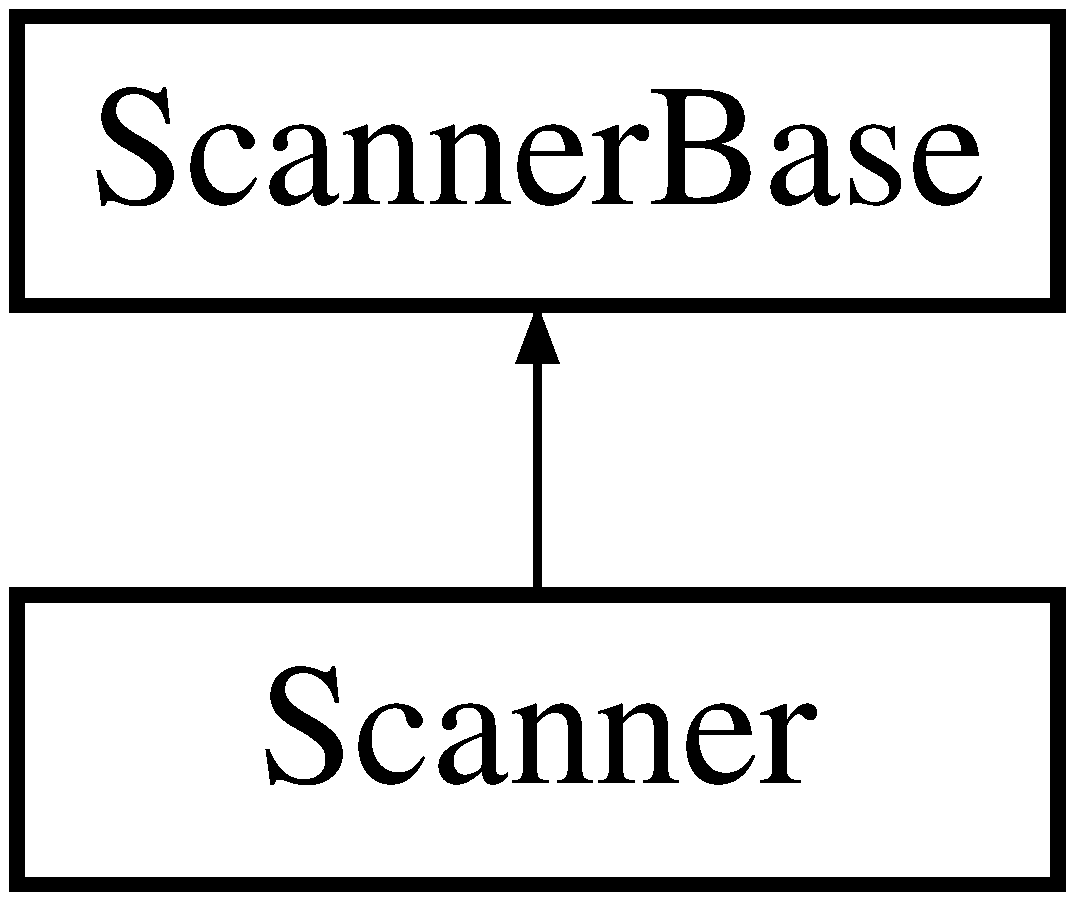
\includegraphics[height=2.000000cm]{classScanner}
\end{center}
\end{figure}
\subsection*{Public Member Functions}
\begin{DoxyCompactItemize}
\item 
\hypertarget{classScanner_a2987a0c6aba4250e6cb1c84453d682ff}{{\bfseries Scanner} (std\+::istream \&in=std\+::cin, std\+::ostream \&out=std\+::cout)}\label{classScanner_a2987a0c6aba4250e6cb1c84453d682ff}

\item 
\hypertarget{classScanner_ad27971ec11ede59d0b041284306b6d1f}{{\bfseries Scanner} (std\+::string const \&infile, std\+::string const \&outfile)}\label{classScanner_ad27971ec11ede59d0b041284306b6d1f}

\item 
\hypertarget{classScanner_a6fa640fdbafd7b173be91598708d26a4}{int {\bfseries lex} ()}\label{classScanner_a6fa640fdbafd7b173be91598708d26a4}

\end{DoxyCompactItemize}
\subsection*{Additional Inherited Members}


The documentation for this class was generated from the following files\+:\begin{DoxyCompactItemize}
\item 
scanner/Scanner.\+h\item 
scanner/lex.\+cc\end{DoxyCompactItemize}

\hypertarget{classScannerBase}{\section{Scanner\+Base Class Reference}
\label{classScannerBase}\index{Scanner\+Base@{Scanner\+Base}}
}
Inheritance diagram for Scanner\+Base\+:\begin{figure}[H]
\begin{center}
\leavevmode
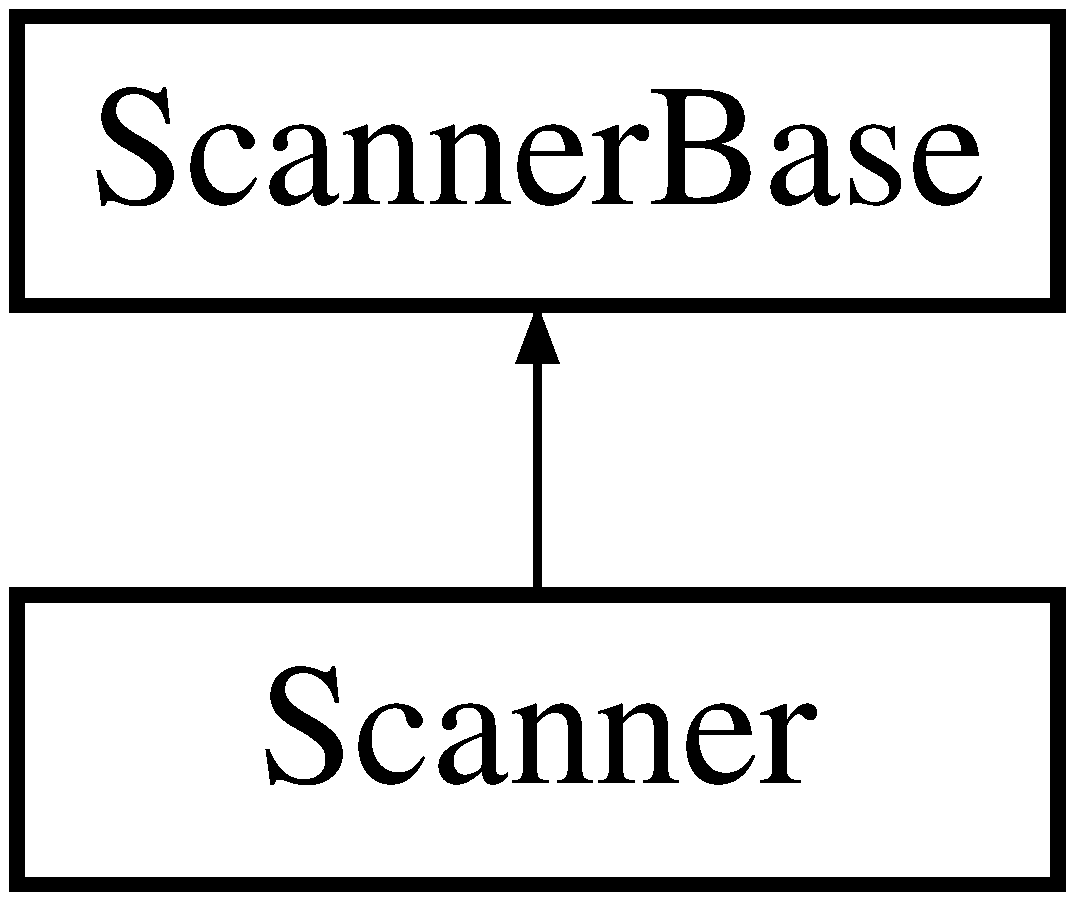
\includegraphics[height=2.000000cm]{classScannerBase}
\end{center}
\end{figure}
\subsection*{Classes}
\begin{DoxyCompactItemize}
\item 
struct \hyperlink{structScannerBase_1_1StreamStruct}{Stream\+Struct}
\end{DoxyCompactItemize}
\subsection*{Public Types}
\begin{DoxyCompactItemize}
\item 
\hypertarget{classScannerBase_a5c7a457813088d6b87650032becad324}{enum {\bfseries Start\+Condition\+\_\+\+\_\+} \{ {\bfseries I\+N\+I\+T\+I\+A\+L}
 \}}\label{classScannerBase_a5c7a457813088d6b87650032becad324}

\end{DoxyCompactItemize}
\subsection*{Public Member Functions}
\begin{DoxyCompactItemize}
\item 
\hypertarget{classScannerBase_a52dace818f491ca943e37e5dafd4c61a}{{\bfseries Scanner\+Base} (\hyperlink{classScannerBase}{Scanner\+Base} const \&other)=delete}\label{classScannerBase_a52dace818f491ca943e37e5dafd4c61a}

\item 
\hypertarget{classScannerBase_a8bba721b91214ec1c7f08d8602789ee9}{\hyperlink{classScannerBase}{Scanner\+Base} \& {\bfseries operator=} (\hyperlink{classScannerBase}{Scanner\+Base} const \&rhs)=delete}\label{classScannerBase_a8bba721b91214ec1c7f08d8602789ee9}

\item 
\hypertarget{classScannerBase_a77130b2ae81f92960bfd49c7fcf05d8d}{bool {\bfseries debug} () const }\label{classScannerBase_a77130b2ae81f92960bfd49c7fcf05d8d}

\item 
\hypertarget{classScannerBase_ab23eaadc4d45bdc3b67226f9010e836b}{std\+::string const \& {\bfseries filename} () const }\label{classScannerBase_ab23eaadc4d45bdc3b67226f9010e836b}

\item 
\hypertarget{classScannerBase_a13c5167ad30e8d89b181ceb40b91a9b7}{std\+::string const \& {\bfseries matched} () const }\label{classScannerBase_a13c5167ad30e8d89b181ceb40b91a9b7}

\item 
\hypertarget{classScannerBase_ad9ad6a5818e6f37d05e6c8b06afcd90b}{size\+\_\+t {\bfseries length} () const }\label{classScannerBase_ad9ad6a5818e6f37d05e6c8b06afcd90b}

\item 
\hypertarget{classScannerBase_ab55926b7d06e99f1d3a8cd410cc544aa}{size\+\_\+t {\bfseries line\+Nr} () const }\label{classScannerBase_ab55926b7d06e99f1d3a8cd410cc544aa}

\item 
\hypertarget{classScannerBase_aef0df93b2a8d97fb61a5d282bddad859}{void {\bfseries set\+Debug} (bool on\+Off)}\label{classScannerBase_aef0df93b2a8d97fb61a5d282bddad859}

\item 
\hypertarget{classScannerBase_a6248d6f0d8ac1926a3666a1542390370}{void {\bfseries switch\+Ostream} (std\+::ostream \&out)}\label{classScannerBase_a6248d6f0d8ac1926a3666a1542390370}

\item 
\hypertarget{classScannerBase_a8afc45efc1ed7b3d3c72ed10abf9042e}{void {\bfseries switch\+Ostream} (std\+::string const \&outfilename)}\label{classScannerBase_a8afc45efc1ed7b3d3c72ed10abf9042e}

\item 
\hypertarget{classScannerBase_a4055b5f788140f12de27708c2a451860}{void {\bfseries switch\+Streams} (std\+::istream \&in, std\+::ostream \&out=std\+::cout)}\label{classScannerBase_a4055b5f788140f12de27708c2a451860}

\item 
\hypertarget{classScannerBase_af2124b7be3b7ff080409983ed54704f3}{void {\bfseries switch\+Istream} (std\+::string const \&infilename)}\label{classScannerBase_af2124b7be3b7ff080409983ed54704f3}

\item 
\hypertarget{classScannerBase_ac5badcfe2ac5fb640a8c18b2fe8c4a41}{void {\bfseries switch\+Streams} (std\+::string const \&infilename, std\+::string const \&outfilename)}\label{classScannerBase_ac5badcfe2ac5fb640a8c18b2fe8c4a41}

\end{DoxyCompactItemize}
\subsection*{Protected Types}
\begin{DoxyCompactItemize}
\item 
\hypertarget{classScannerBase_aba19fcbdd61aaa668cd65fd00ef856f5}{enum {\bfseries Leave\+\_\+\+\_\+} }\label{classScannerBase_aba19fcbdd61aaa668cd65fd00ef856f5}

\item 
\hypertarget{classScannerBase_aeca9da0ddb2e5928570501a6354d7fca}{enum {\bfseries Action\+Type\+\_\+\+\_\+} \{ \\*
{\bfseries C\+O\+N\+T\+I\+N\+U\+E}, 
{\bfseries E\+C\+H\+O\+\_\+\+C\+H}, 
{\bfseries E\+C\+H\+O\+\_\+\+F\+I\+R\+S\+T}, 
{\bfseries M\+A\+T\+C\+H}, 
\\*
{\bfseries R\+E\+T\+U\+R\+N}
 \}}\label{classScannerBase_aeca9da0ddb2e5928570501a6354d7fca}

\item 
\hypertarget{classScannerBase_a6b05193c90b76c2923c127381f3f487a}{enum {\bfseries Post\+Enum\+\_\+\+\_\+} \{ {\bfseries E\+N\+D}, 
{\bfseries P\+O\+P}, 
{\bfseries R\+E\+T\+U\+R\+N}, 
{\bfseries W\+I\+P}
 \}}\label{classScannerBase_a6b05193c90b76c2923c127381f3f487a}

\item 
\hypertarget{classScannerBase_a05438c73aa59e8fdcd61d6c46087d3fd}{enum \+: bool \{ {\bfseries s\+\_\+interactive\+\_\+\+\_\+} = false
 \}}\label{classScannerBase_a05438c73aa59e8fdcd61d6c46087d3fd}

\item 
\hypertarget{classScannerBase_ace58cd1a2ba5ff08fb6c6460cabe6f2e}{enum \+: size\+\_\+t \{ {\bfseries s\+\_\+range\+Of\+E\+O\+F\+\_\+\+\_\+} = 57, 
{\bfseries s\+\_\+fin\+Idx\+\_\+\+\_\+} = 58, 
{\bfseries s\+\_\+n\+Rules\+\_\+\+\_\+} = 113, 
{\bfseries s\+\_\+max\+Sizeof\+Stream\+Stack\+\_\+\+\_\+} = 10
 \}}\label{classScannerBase_ace58cd1a2ba5ff08fb6c6460cabe6f2e}

\end{DoxyCompactItemize}
\subsection*{Protected Member Functions}
\begin{DoxyCompactItemize}
\item 
\hypertarget{classScannerBase_a314e6672cca5961b1cf293017c2778e8}{{\bfseries Scanner\+Base} (std\+::istream \&in, std\+::ostream \&out)}\label{classScannerBase_a314e6672cca5961b1cf293017c2778e8}

\item 
\hypertarget{classScannerBase_adab6f6482546225266827314d4faa4cd}{{\bfseries Scanner\+Base} (std\+::string const \&infilename, std\+::string const \&outfilename)}\label{classScannerBase_adab6f6482546225266827314d4faa4cd}

\item 
\hypertarget{classScannerBase_af594ada5dd8676cfeb8adb5c2aef6ef5}{Start\+Condition\+\_\+\+\_\+ {\bfseries start\+Condition} () const }\label{classScannerBase_af594ada5dd8676cfeb8adb5c2aef6ef5}

\item 
\hypertarget{classScannerBase_a01dfe058b5b337e03aed1012ad9dc002}{bool {\bfseries pop\+Stream} ()}\label{classScannerBase_a01dfe058b5b337e03aed1012ad9dc002}

\item 
\hypertarget{classScannerBase_aa6adde433468e75c4c10b69bca1049d9}{std\+::ostream \& {\bfseries out} ()}\label{classScannerBase_aa6adde433468e75c4c10b69bca1049d9}

\item 
\hypertarget{classScannerBase_a29c66509f23640290421589481d8a388}{void {\bfseries begin} (Start\+Condition\+\_\+\+\_\+ start\+Condition)}\label{classScannerBase_a29c66509f23640290421589481d8a388}

\item 
\hypertarget{classScannerBase_a911243f589c4eaa97578fa6f37916e75}{void {\bfseries echo} () const }\label{classScannerBase_a911243f589c4eaa97578fa6f37916e75}

\item 
\hypertarget{classScannerBase_a186091b02e0982d066a1b187c5bc6894}{void {\bfseries leave} (int ret\+Value) const }\label{classScannerBase_a186091b02e0982d066a1b187c5bc6894}

\item 
\hypertarget{classScannerBase_a18d6405c9ccd130c8176326f728841b2}{void {\bfseries accept} (size\+\_\+t n\+Chars=0)}\label{classScannerBase_a18d6405c9ccd130c8176326f728841b2}

\item 
\hypertarget{classScannerBase_ae1cdca0b7158f331448e744496ef2ccd}{void {\bfseries redo} (size\+\_\+t n\+Chars=0)}\label{classScannerBase_ae1cdca0b7158f331448e744496ef2ccd}

\item 
\hypertarget{classScannerBase_aac0eac4274996b1dbe96c25b7a72c291}{void {\bfseries more} ()}\label{classScannerBase_aac0eac4274996b1dbe96c25b7a72c291}

\item 
\hypertarget{classScannerBase_aaac7ba2745723f9c32fe73be62ccabe7}{void {\bfseries push} (size\+\_\+t ch)}\label{classScannerBase_aaac7ba2745723f9c32fe73be62ccabe7}

\item 
\hypertarget{classScannerBase_a560981768e4742beca13cd499ac2aee6}{void {\bfseries push} (std\+::string const \&txt)}\label{classScannerBase_a560981768e4742beca13cd499ac2aee6}

\item 
\hypertarget{classScannerBase_a6f27a6435c98c739507207f17e71bc86}{std\+::vector$<$ \hyperlink{structScannerBase_1_1StreamStruct}{Stream\+Struct} $>$ const \& {\bfseries stream\+Stack} () const }\label{classScannerBase_a6f27a6435c98c739507207f17e71bc86}

\item 
\hypertarget{classScannerBase_a7a5b3ba90f7c325382b7e8b740f68b84}{void {\bfseries push\+Stream} (std\+::istream \&cur\+Stream)}\label{classScannerBase_a7a5b3ba90f7c325382b7e8b740f68b84}

\item 
\hypertarget{classScannerBase_abd859aa5cf970c528f9619e4a7dcdd3d}{void {\bfseries push\+Stream} (std\+::string const \&cur\+Name)}\label{classScannerBase_abd859aa5cf970c528f9619e4a7dcdd3d}

\item 
\hypertarget{classScannerBase_abef7b7162ed50674ceb6e8ea97997ecd}{void {\bfseries set\+Filename} (std\+::string const \&name)}\label{classScannerBase_abef7b7162ed50674ceb6e8ea97997ecd}

\item 
\hypertarget{classScannerBase_a255420f4d51d5ffcb8c6a2447e92b4db}{void {\bfseries set\+Matched} (std\+::string const \&text)}\label{classScannerBase_a255420f4d51d5ffcb8c6a2447e92b4db}

\item 
\hypertarget{classScannerBase_a22a9d4fa2238f4e805943f8fe8f771db}{Action\+Type\+\_\+\+\_\+ {\bfseries action\+Type\+\_\+\+\_\+} (size\+\_\+t range)}\label{classScannerBase_a22a9d4fa2238f4e805943f8fe8f771db}

\item 
\hypertarget{classScannerBase_abacd35ee1ba9ef1afddba760bcf73e24}{bool {\bfseries return\+\_\+\+\_\+} ()}\label{classScannerBase_abacd35ee1ba9ef1afddba760bcf73e24}

\item 
\hypertarget{classScannerBase_a0dc1bb7170d2c62164e8aaaa4fdb4bfa}{size\+\_\+t {\bfseries matched\+\_\+\+\_\+} (size\+\_\+t ch)}\label{classScannerBase_a0dc1bb7170d2c62164e8aaaa4fdb4bfa}

\item 
\hypertarget{classScannerBase_a9cdbc8de197e589b53b9d813cb398427}{size\+\_\+t {\bfseries get\+Range\+\_\+\+\_\+} (int ch)}\label{classScannerBase_a9cdbc8de197e589b53b9d813cb398427}

\item 
\hypertarget{classScannerBase_a7f1dbe1f9c0bc8ad210eeff600d87818}{size\+\_\+t {\bfseries get\+\_\+\+\_\+} ()}\label{classScannerBase_a7f1dbe1f9c0bc8ad210eeff600d87818}

\item 
\hypertarget{classScannerBase_ad686a6aad34bb9eb160ea71f3ceff6cd}{size\+\_\+t {\bfseries state\+\_\+\+\_\+} () const }\label{classScannerBase_ad686a6aad34bb9eb160ea71f3ceff6cd}

\item 
\hypertarget{classScannerBase_ad57bbe8f2362d83aee7203979eaf5b4b}{void {\bfseries continue\+\_\+\+\_\+} (int ch)}\label{classScannerBase_ad57bbe8f2362d83aee7203979eaf5b4b}

\item 
\hypertarget{classScannerBase_ae3297769b30f01d67734a5d73c19edf3}{void {\bfseries echo\+Ch\+\_\+\+\_\+} (size\+\_\+t ch)}\label{classScannerBase_ae3297769b30f01d67734a5d73c19edf3}

\item 
\hypertarget{classScannerBase_ad23055462d6988c8d68cb5876846333a}{void {\bfseries echo\+First\+\_\+\+\_\+} (size\+\_\+t ch)}\label{classScannerBase_ad23055462d6988c8d68cb5876846333a}

\item 
\hypertarget{classScannerBase_a3cb757b8ea955d005524b441400d4307}{void {\bfseries update\+Finals\+\_\+\+\_\+} ()}\label{classScannerBase_a3cb757b8ea955d005524b441400d4307}

\item 
\hypertarget{classScannerBase_ac74c722b9ed9350c2579de9a278e8917}{void {\bfseries no\+Return\+\_\+\+\_\+} ()}\label{classScannerBase_ac74c722b9ed9350c2579de9a278e8917}

\item 
\hypertarget{classScannerBase_a9f3016ad3dd153084338996814517860}{void {\bfseries print\+\_\+\+\_\+} () const }\label{classScannerBase_a9f3016ad3dd153084338996814517860}

\item 
\hypertarget{classScannerBase_a93bc4ebf1066dcc078f92ca46c2ac06c}{void {\bfseries push\+Front\+\_\+\+\_\+} (size\+\_\+t ch)}\label{classScannerBase_a93bc4ebf1066dcc078f92ca46c2ac06c}

\item 
\hypertarget{classScannerBase_a68143fa375f40372a20a341fbd29add8}{void {\bfseries reset\+\_\+\+\_\+} ()}\label{classScannerBase_a68143fa375f40372a20a341fbd29add8}

\item 
\hypertarget{classScannerBase_ae47bc161d7895da37aae6365b4c8cef7}{void {\bfseries switch\+Stream\+\_\+\+\_\+} (std\+::istream \&in, size\+\_\+t line\+Nr)}\label{classScannerBase_ae47bc161d7895da37aae6365b4c8cef7}

\item 
\hypertarget{classScannerBase_a9635171f8d89e43eaa6bb035e302e2a3}{void {\bfseries lopf\+\_\+\+\_\+} (size\+\_\+t tail)}\label{classScannerBase_a9635171f8d89e43eaa6bb035e302e2a3}

\item 
\hypertarget{classScannerBase_a7002587b47a5f2d1e4be6a530c7076a7}{void {\bfseries lop1\+\_\+\+\_\+} (int lop\+S\+C)}\label{classScannerBase_a7002587b47a5f2d1e4be6a530c7076a7}

\item 
\hypertarget{classScannerBase_a93a25cf1505db9a9a0f3dd4fb9a40c51}{void {\bfseries lop2\+\_\+\+\_\+} ()}\label{classScannerBase_a93a25cf1505db9a9a0f3dd4fb9a40c51}

\item 
\hypertarget{classScannerBase_a812266cffb3ddd6f1ff64d2ee8151e78}{void {\bfseries lop3\+\_\+\+\_\+} ()}\label{classScannerBase_a812266cffb3ddd6f1ff64d2ee8151e78}

\item 
\hypertarget{classScannerBase_abf3fb2a9582ea160dd19439667997a95}{void {\bfseries lop4\+\_\+\+\_\+} ()}\label{classScannerBase_abf3fb2a9582ea160dd19439667997a95}

\end{DoxyCompactItemize}
\subsection*{Static Protected Member Functions}
\begin{DoxyCompactItemize}
\item 
\hypertarget{classScannerBase_a9dcc3f8c186983bc1ea3d7541e231c8b}{static std\+::string {\bfseries istream\+Name\+\_\+\+\_\+} ()}\label{classScannerBase_a9dcc3f8c186983bc1ea3d7541e231c8b}

\end{DoxyCompactItemize}
\subsection*{Protected Attributes}
\begin{DoxyCompactItemize}
\item 
\hypertarget{classScannerBase_a642557896ede13c5abcf760451d8f4e4}{std\+::istream $\ast$ {\bfseries d\+\_\+in\+\_\+\+\_\+}}\label{classScannerBase_a642557896ede13c5abcf760451d8f4e4}

\item 
\hypertarget{classScannerBase_a72375048231dd617b0cf5bc9e6082eb2}{int {\bfseries d\+\_\+token\+\_\+\+\_\+}}\label{classScannerBase_a72375048231dd617b0cf5bc9e6082eb2}

\item 
\hypertarget{classScannerBase_aabb7825e2871ae7562dbe7e4af52b612}{int const ($\ast$ {\bfseries d\+\_\+dfa\+Base\+\_\+\+\_\+} )\mbox{[}60\mbox{]}}\label{classScannerBase_aabb7825e2871ae7562dbe7e4af52b612}

\end{DoxyCompactItemize}
\subsection*{Static Protected Attributes}
\begin{DoxyCompactItemize}
\item 
\hypertarget{classScannerBase_ab685af9cad317918294c24eb6dc8deb7}{static int const {\bfseries s\+\_\+dfa\+\_\+\+\_\+} \mbox{[}$\,$\mbox{]}\mbox{[}60\mbox{]}}\label{classScannerBase_ab685af9cad317918294c24eb6dc8deb7}

\item 
\hypertarget{classScannerBase_ac6b8b447499524147c97f3eccf9760fd}{static int const ($\ast$\mbox{[}$\,$\mbox{]} {\bfseries s\+\_\+dfa\+Base\+\_\+\+\_\+} )\mbox{[}60\mbox{]}}\label{classScannerBase_ac6b8b447499524147c97f3eccf9760fd}

\item 
static size\+\_\+t const {\bfseries s\+\_\+ranges\+\_\+\+\_\+} \mbox{[}$\,$\mbox{]}
\item 
\hypertarget{classScannerBase_a57a3ac6c72eff17211c2e58fc4eafb80}{static size\+\_\+t const {\bfseries s\+\_\+rf\+\_\+\+\_\+} \mbox{[}$\,$\mbox{]}\mbox{[}2\mbox{]}}\label{classScannerBase_a57a3ac6c72eff17211c2e58fc4eafb80}

\end{DoxyCompactItemize}


\subsection{Member Data Documentation}
\hypertarget{classScannerBase_a900ba43aca6a632d3eb27a17b3f34834}{\index{Scanner\+Base@{Scanner\+Base}!s\+\_\+ranges\+\_\+\+\_\+@{s\+\_\+ranges\+\_\+\+\_\+}}
\index{s\+\_\+ranges\+\_\+\+\_\+@{s\+\_\+ranges\+\_\+\+\_\+}!Scanner\+Base@{Scanner\+Base}}
\subsubsection[{s\+\_\+ranges\+\_\+\+\_\+}]{\setlength{\rightskip}{0pt plus 5cm}size\+\_\+t const Scanner\+Base\+::s\+\_\+ranges\+\_\+\+\_\+\hspace{0.3cm}{\ttfamily [static]}, {\ttfamily [protected]}}}\label{classScannerBase_a900ba43aca6a632d3eb27a17b3f34834}
{\bfseries Initial value\+:}
\begin{DoxyCode}
=
\{
     0, 0, 0, 0, 0, 0, 0, 0, 0, 1, 2, 3, 3, 3, 3, 3, 3, 3, 3, 3, 3, 3, 3, 3, 3,
     3, 3, 3, 3, 3, 3, 3, 4, 5, 5, 6, 7, 7, 7, 7, 8, 9,10,11,12,13,14,15,16,16,
    16,16,16,16,16,16,16,16,17,18,19,20,21,22,23,24,24,24,24,24,24,24,24,24,24,
    24,24,24,24,24,24,24,24,24,24,24,24,24,24,24,24,25,26,27,28,28,29,30,31,32,
    33,34,35,36,37,38,39,40,41,42,43,44,45,46,47,48,49,50,51,52,53,54,55,56,56,
    56,56,56,56,56,56,56,56,56,56,56,56,56,56,56,56,56,56,56,56,56,56,56,56,56,
    56,56,56,56,56,56,56,56,56,56,56,56,56,56,56,56,56,56,56,56,56,56,56,56,56,
    56,56,56,56,56,56,56,56,56,56,56,56,56,56,56,56,56,56,56,56,56,56,56,56,56,
    56,56,56,56,56,56,56,56,56,56,56,56,56,56,56,56,56,56,56,56,56,56,56,56,56,
    56,56,56,56,56,56,56,56,56,56,56,56,56,56,56,56,56,56,56,56,56,56,56,56,56,
    56,56,56,56,56,56,
\}
\end{DoxyCode}


The documentation for this class was generated from the following files\+:\begin{DoxyCompactItemize}
\item 
scanner/Scannerbase.\+h\item 
scanner/lex.\+cc\end{DoxyCompactItemize}

\hypertarget{structScannerBase_1_1StreamStruct}{\section{Scanner\+Base\+:\+:Stream\+Struct Struct Reference}
\label{structScannerBase_1_1StreamStruct}\index{Scanner\+Base\+::\+Stream\+Struct@{Scanner\+Base\+::\+Stream\+Struct}}
}
\subsection*{Public Attributes}
\begin{DoxyCompactItemize}
\item 
\hypertarget{structScannerBase_1_1StreamStruct_a890dab2308ed9ceb65355336397fe0b3}{std\+::string {\bfseries pushed\+Name}}\label{structScannerBase_1_1StreamStruct_a890dab2308ed9ceb65355336397fe0b3}

\item 
\hypertarget{structScannerBase_1_1StreamStruct_a188ad02b8ba4d1442f21a100dcd3ea63}{Input {\bfseries pushed\+Input}}\label{structScannerBase_1_1StreamStruct_a188ad02b8ba4d1442f21a100dcd3ea63}

\end{DoxyCompactItemize}


The documentation for this struct was generated from the following file\+:\begin{DoxyCompactItemize}
\item 
scanner/Scannerbase.\+h\end{DoxyCompactItemize}

\hypertarget{unionParserBase_1_1STYPE____}{\section{Parser\+Base\+:\+:S\+T\+Y\+P\+E\+\_\+\+\_\+ Union Reference}
\label{unionParserBase_1_1STYPE____}\index{Parser\+Base\+::\+S\+T\+Y\+P\+E\+\_\+\+\_\+@{Parser\+Base\+::\+S\+T\+Y\+P\+E\+\_\+\+\_\+}}
}
\subsection*{Public Attributes}
\begin{DoxyCompactItemize}
\item 
\hypertarget{unionParserBase_1_1STYPE_____af8152366c391a9a3c6dfeebd38dd6072}{int {\bfseries integer}}\label{unionParserBase_1_1STYPE_____af8152366c391a9a3c6dfeebd38dd6072}

\item 
\hypertarget{unionParserBase_1_1STYPE_____a3d0cb98bf31057ecd7a908afbe3ca55f}{float {\bfseries number}}\label{unionParserBase_1_1STYPE_____a3d0cb98bf31057ecd7a908afbe3ca55f}

\item 
\hypertarget{unionParserBase_1_1STYPE_____af9a7a51fe1e387c4c8214d7942e2a58a}{std\+::string $\ast$ {\bfseries name}}\label{unionParserBase_1_1STYPE_____af9a7a51fe1e387c4c8214d7942e2a58a}

\item 
\hypertarget{unionParserBase_1_1STYPE_____acadc01542881f7e6add2ea0e05562e8b}{std\+::vector$<$ std\+::string $>$ $\ast$ {\bfseries list\+\_\+name}}\label{unionParserBase_1_1STYPE_____acadc01542881f7e6add2ea0e05562e8b}

\item 
\hypertarget{unionParserBase_1_1STYPE_____a4bd64b9de1820c87495a8bd2c914e9ad}{std\+::vector$<$ float $>$ $\ast$ {\bfseries list\+\_\+float}}\label{unionParserBase_1_1STYPE_____a4bd64b9de1820c87495a8bd2c914e9ad}

\item 
\hypertarget{unionParserBase_1_1STYPE_____a96b9185e300e325c901f02ab6c4b3297}{std\+::pair$<$ std\+::vector\\*
$<$ std\+::string $>$ $\ast$, std\+::string $\ast$ $>$ $\ast$ {\bfseries atomic\+\_\+formula}}\label{unionParserBase_1_1STYPE_____a96b9185e300e325c901f02ab6c4b3297}

\item 
\hypertarget{unionParserBase_1_1STYPE_____a931331d6fc1c63176aface5775f7973d}{std\+::vector$<$ \hyperlink{classTypedList}{Typed\+List} $\ast$ $>$ $\ast$ {\bfseries typed\+List\+\_\+list}}\label{unionParserBase_1_1STYPE_____a931331d6fc1c63176aface5775f7973d}

\item 
\hypertarget{unionParserBase_1_1STYPE_____ae6657530c88b67602d9c3d152c9e08bb}{std\+::pair$<$ std\+::string \\*
$\ast$, std\+::vector$<$ \hyperlink{classTypedList}{Typed\+List} $\ast$ $>$ $\ast$ $>$ $\ast$ {\bfseries function\+\_\+skeleton}}\label{unionParserBase_1_1STYPE_____ae6657530c88b67602d9c3d152c9e08bb}

\item 
\hypertarget{unionParserBase_1_1STYPE_____ac3322fdc19571ded0354accbb53384cb}{std\+::vector$<$ std\+::pair\\*
$<$ std\+::string $\ast$, std\+::vector\\*
$<$ \hyperlink{classTypedList}{Typed\+List} $\ast$ $>$ $\ast$ $>$ $\ast$ $>$ $\ast$ {\bfseries function\+\_\+skeleton\+\_\+list}}\label{unionParserBase_1_1STYPE_____ac3322fdc19571ded0354accbb53384cb}

\item 
\hypertarget{unionParserBase_1_1STYPE_____a70c36b4ca4cb9695e912495b0a276b63}{std\+::pair$<$ std\+::pair\\*
$<$ std\+::vector$<$ std\+::string $>$\\*
 $\ast$, std\+::string $\ast$ $>$ $\ast$, bool $>$ $\ast$ {\bfseries literal}}\label{unionParserBase_1_1STYPE_____a70c36b4ca4cb9695e912495b0a276b63}

\item 
\hypertarget{unionParserBase_1_1STYPE_____a4b65f160ac88f1f44a1e9c4a892b3612}{std\+::vector$<$ std\+::vector\\*
$<$ std\+::pair$<$ std\+::pair\\*
$<$ std\+::vector$<$ std\+::string $>$\\*
 $\ast$, std\+::string $\ast$ $>$ $\ast$, int $>$ $\ast$ $>$ $\ast$ $>$ $\ast$ {\bfseries pre\+\_\+\+G\+D}}\label{unionParserBase_1_1STYPE_____a4b65f160ac88f1f44a1e9c4a892b3612}

\item 
\hypertarget{unionParserBase_1_1STYPE_____adf129a6213d541035b873cff52d26e63}{std\+::vector$<$ std\+::pair\\*
$<$ std\+::pair$<$ std\+::vector\\*
$<$ std\+::string $>$ $\ast$, std\+::string $\ast$ $>$\\*
 $\ast$, int $>$ $\ast$ $>$ $\ast$ {\bfseries timed\+\_\+\+G\+D}}\label{unionParserBase_1_1STYPE_____adf129a6213d541035b873cff52d26e63}

\item 
\hypertarget{unionParserBase_1_1STYPE_____a79e1c1d70b78c5bd090118c2fbf46781}{std\+::vector$<$ std\+::pair\\*
$<$ std\+::pair$<$ std\+::vector\\*
$<$ std\+::string $>$ $\ast$, std\+::string $\ast$ $>$\\*
 $\ast$, int $>$ $\ast$ $>$ $\ast$ {\bfseries cond\+\_\+effect}}\label{unionParserBase_1_1STYPE_____a79e1c1d70b78c5bd090118c2fbf46781}

\item 
\hypertarget{unionParserBase_1_1STYPE_____a3db853e7495c942705760c89cdeaa79e}{std\+::pair$<$ std\+::pair\\*
$<$ std\+::vector$<$ std\+::pair\\*
$<$ std\+::pair$<$ std\+::vector\\*
$<$ std\+::string $>$ $\ast$, std\+::string $\ast$ $>$\\*
 $\ast$, int $>$ $\ast$ $>$ $\ast$, std\+::vector\\*
$<$ std\+::pair$<$ std\+::pair\\*
$<$ std\+::vector$<$ std\+::string $>$\\*
 $\ast$, std\+::string $\ast$ $>$ $\ast$, int $>$\\*
 $\ast$ $>$ $\ast$ $>$ $\ast$, float $>$ $\ast$ {\bfseries da\+\_\+def\+\_\+body}}\label{unionParserBase_1_1STYPE_____a3db853e7495c942705760c89cdeaa79e}

\end{DoxyCompactItemize}


The documentation for this union was generated from the following file\+:\begin{DoxyCompactItemize}
\item 
parser/Parserbase.\+h\end{DoxyCompactItemize}

\hypertarget{classTlpgp1}{\section{Tlpgp1 Class Reference}
\label{classTlpgp1}\index{Tlpgp1@{Tlpgp1}}
}
\subsection*{Public Member Functions}
\begin{DoxyCompactItemize}
\item 
\hypertarget{classTlpgp1_a3b25a7a10b2c57010a1b840a45fc8f3e}{{\bfseries Tlpgp1} (\hyperlink{classDomain}{Domain} $\ast$domain, \hyperlink{classProblem}{Problem} $\ast$problem)}\label{classTlpgp1_a3b25a7a10b2c57010a1b840a45fc8f3e}

\item 
\hypertarget{classTlpgp1_aa11e139d77987da500f752fd865a72e6}{void \hyperlink{classTlpgp1_aa11e139d77987da500f752fd865a72e6}{construct\+Graph} ()}\label{classTlpgp1_aa11e139d77987da500f752fd865a72e6}

\begin{DoxyCompactList}\small\item\em tlpgp1 core function \end{DoxyCompactList}\item 
\hypertarget{classTlpgp1_ac1f49c011d952f18cc1f5bcc1d87fcea}{void \hyperlink{classTlpgp1_ac1f49c011d952f18cc1f5bcc1d87fcea}{vertex\+To\+Actions} ()}\label{classTlpgp1_ac1f49c011d952f18cc1f5bcc1d87fcea}

\begin{DoxyCompactList}\small\item\em converts a graph into an vector of vector ($\ast$father,vector of actions) -\/$>$ (vector$<$vector action$>$) \end{DoxyCompactList}\end{DoxyCompactItemize}


The documentation for this class was generated from the following files\+:\begin{DoxyCompactItemize}
\item 
src/\hyperlink{tlpgp1_8h}{tlpgp1.\+h}\item 
src/\hyperlink{tlpgp1_8cpp}{tlpgp1.\+cpp}\end{DoxyCompactItemize}

\hypertarget{classTlpgp2}{\section{Tlpgp2 Class Reference}
\label{classTlpgp2}\index{Tlpgp2@{Tlpgp2}}
}
\subsection*{Public Member Functions}
\begin{DoxyCompactItemize}
\item 
\hypertarget{classTlpgp2_aaf6e32a58dfd9128a90ea596851c1a1e}{{\bfseries Tlpgp2} (\hyperlink{classVertex}{Vertex} $\ast$vertex)}\label{classTlpgp2_aaf6e32a58dfd9128a90ea596851c1a1e}

\item 
\hypertarget{classTlpgp2_ab4d91ec45b002a4b53156d842f212111}{string {\bfseries generate\+Graph\+Smt2} ()}\label{classTlpgp2_ab4d91ec45b002a4b53156d842f212111}

\item 
\hypertarget{classTlpgp2_aed8a6242238a73eea2dc091ddd547bac}{string {\bfseries namelink\+Prec} (string name, \hyperlink{classFluent}{Fluent} $\ast$fluent, \hyperlink{classAttribute}{Attribute} att, \hyperlink{classVertex}{Vertex} $\ast$vertex, int state)}\label{classTlpgp2_aed8a6242238a73eea2dc091ddd547bac}

\item 
\hypertarget{classTlpgp2_a743100501d2300321b164df27b213c81}{string {\bfseries link\+Prec} (string name, \hyperlink{classFluent}{Fluent} $\ast$fluent, \hyperlink{classAttribute}{Attribute} att, \hyperlink{classVertex}{Vertex} $\ast$vertex, int state)}\label{classTlpgp2_a743100501d2300321b164df27b213c81}

\item 
\hypertarget{classTlpgp2_a8feeba8c8905b6589503aab75c7aa163}{string {\bfseries protect\+Cond} (string link, \hyperlink{classFluent}{Fluent} $\ast$fluent, \hyperlink{classAttribute}{Attribute} att, string nameb, string namet)}\label{classTlpgp2_a8feeba8c8905b6589503aab75c7aa163}

\item 
\hypertarget{classTlpgp2_ad328b4c1c7b4d5c0f0b8de682e52e582}{bool {\bfseries compare\+V\+V} (vector$<$ \hyperlink{classMember}{Member} $\ast$ $>$ $\ast$v1, vector$<$ \hyperlink{classMember}{Member} $\ast$ $>$ $\ast$v2)}\label{classTlpgp2_ad328b4c1c7b4d5c0f0b8de682e52e582}

\item 
\hypertarget{classTlpgp2_ad2b83e2998d8206661d309c4105d237a}{string {\bfseries protect\+Effect} (string name, \hyperlink{classDurativeAction}{Durative\+Action} $\ast$a, \hyperlink{classFluent}{Fluent} $\ast$fluent, \hyperlink{classAttribute}{Attribute} att, int statep)}\label{classTlpgp2_ad2b83e2998d8206661d309c4105d237a}

\end{DoxyCompactItemize}


The documentation for this class was generated from the following files\+:\begin{DoxyCompactItemize}
\item 
src/tlpgp2.\+h\item 
src/tlpgp2.\+cpp\end{DoxyCompactItemize}

\hypertarget{classTools}{\section{Tools Class Reference}
\label{classTools}\index{Tools@{Tools}}
}
\subsection*{Public Member Functions}
\begin{DoxyCompactItemize}
\item 
\hypertarget{classTools_a82964e604c52b7a2250e8a5291fae80d}{bool {\bfseries is\+In} (\hyperlink{classType}{Type} $\ast$t, vector$<$ \hyperlink{classType}{Type} $\ast$ $>$ $\ast$v)}\label{classTools_a82964e604c52b7a2250e8a5291fae80d}

\item 
\hypertarget{classTools_a133831bc0b6c2c426a2beef303fe31d8}{bool {\bfseries compare\+Vector\+Type} (vector$<$ \hyperlink{classType}{Type} $\ast$ $>$ $\ast$v1, vector$<$ \hyperlink{classType}{Type} $\ast$ $>$ $\ast$v2)}\label{classTools_a133831bc0b6c2c426a2beef303fe31d8}

\item 
\hypertarget{classTools_a41b2b26e2a03197393e19907c4ab604b}{bool {\bfseries compare\+Action\+Vaction} (\hyperlink{classDurativeAction}{Durative\+Action} $\ast$action, vector$<$ \hyperlink{classDurativeAction}{Durative\+Action} $\ast$ $>$ $\ast$v)}\label{classTools_a41b2b26e2a03197393e19907c4ab604b}

\item 
\hypertarget{classTools_a3e90b6d57c7bf280e371c866c74a804a}{bool {\bfseries solveur} ()}\label{classTools_a3e90b6d57c7bf280e371c866c74a804a}

\item 
\hypertarget{classTools_a3f0feaba003f037f5b45deb00b92099a}{bool {\bfseries compare\+V\+V} (vector$<$ \hyperlink{classMember}{Member} $\ast$ $>$ $\ast$v1, vector$<$ \hyperlink{classMember}{Member} $\ast$ $>$ $\ast$v2)}\label{classTools_a3f0feaba003f037f5b45deb00b92099a}

\item 
\hypertarget{classTools_a23ceae792d59f3abef350ab494b72953}{bool {\bfseries compare\+V\+V2} (vector$<$ \hyperlink{classVariable}{Variable} $>$ $\ast$v1, vector$<$ \hyperlink{classVariable}{Variable} $>$ $\ast$v2)}\label{classTools_a23ceae792d59f3abef350ab494b72953}

\item 
\hypertarget{classTools_af42bb5747bc322664a12860aae3959fc}{bool {\bfseries compare\+A\+A} (\hyperlink{classDurativeAction}{Durative\+Action} $\ast$a1, \hyperlink{classDurativeAction}{Durative\+Action} $\ast$a2)}\label{classTools_af42bb5747bc322664a12860aae3959fc}

\end{DoxyCompactItemize}


The documentation for this class was generated from the following files\+:\begin{DoxyCompactItemize}
\item 
src/tools.\+h\item 
src/tools.\+cpp\end{DoxyCompactItemize}

\hypertarget{classType}{\section{Type Class Reference}
\label{classType}\index{Type@{Type}}
}
\subsection*{Public Member Functions}
\begin{DoxyCompactItemize}
\item 
\hypertarget{classType_a78339313d36891f18427c431ea84e306}{\hyperlink{classType_a78339313d36891f18427c431ea84e306}{Type} ()}\label{classType_a78339313d36891f18427c431ea84e306}

\begin{DoxyCompactList}\small\item\em Constructor. \end{DoxyCompactList}\item 
\hyperlink{classType_aa4810683e26c16eb59e71d28a45e558f}{Type} (string name, vector$<$ \hyperlink{classType}{Type} $\ast$ $>$ parents)
\begin{DoxyCompactList}\small\item\em Constructor. \end{DoxyCompactList}\item 
\hyperlink{classType_a58ff228c4b6fdace44ef1253b06dc51f}{Type} (string name)
\begin{DoxyCompactList}\small\item\em Constructor, the parent type is set to an empty vector. \end{DoxyCompactList}\item 
\hypertarget{classType_a79b5e86eb2dd658180797a1b798194a8}{virtual \hyperlink{classType_a79b5e86eb2dd658180797a1b798194a8}{$\sim$\+Type} ()}\label{classType_a79b5e86eb2dd658180797a1b798194a8}

\begin{DoxyCompactList}\small\item\em Destructor -\/ virtual. \end{DoxyCompactList}\item 
void \hyperlink{classType_aafd68a927632ba693e55737cb56a10ef}{add\+Parents} (vector$<$ \hyperlink{classType}{Type} $\ast$ $>$ parents)
\begin{DoxyCompactList}\small\item\em Add an either type to the existing either type of the parent type (doesn't duplicate) \end{DoxyCompactList}\item 
string \hyperlink{classType_a1a1cd5b58200bf7320bfa663651d185b}{get\+Name} ()
\begin{DoxyCompactList}\small\item\em Get the name of the type. \end{DoxyCompactList}\item 
vector$<$ \hyperlink{classType}{Type} $\ast$ $>$ $\ast$ \hyperlink{classType_a200655820e0067bca4dba0e06857af91}{get\+Parents} ()
\begin{DoxyCompactList}\small\item\em Get the parent of the type. \end{DoxyCompactList}\item 
bool \hyperlink{classType_ae962f493713c0aaadaa891eea97b7424}{is\+One\+Of\+Parents} (string name)
\begin{DoxyCompactList}\small\item\em Check recursively if a type is one the type's parent, in m\+\_\+parents. \end{DoxyCompactList}\item 
string \hyperlink{classType_ab8b2fef62ecd70ff970a0c3e301dc753}{to\+\_\+string} ()
\begin{DoxyCompactList}\small\item\em Return a string that represent the type. \end{DoxyCompactList}\end{DoxyCompactItemize}


\subsection{Constructor \& Destructor Documentation}
\hypertarget{classType_aa4810683e26c16eb59e71d28a45e558f}{\index{Type@{Type}!Type@{Type}}
\index{Type@{Type}!Type@{Type}}
\subsubsection[{Type}]{\setlength{\rightskip}{0pt plus 5cm}Type\+::\+Type (
\begin{DoxyParamCaption}
\item[{string}]{name, }
\item[{vector$<$ {\bf Type} $\ast$ $>$}]{parents}
\end{DoxyParamCaption}
)}}\label{classType_aa4810683e26c16eb59e71d28a45e558f}


Constructor. 


\begin{DoxyParams}{Parameters}
{\em name} & -\/ name of the type parents -\/ either type of the parent \\
\hline
\end{DoxyParams}
\hypertarget{classType_a58ff228c4b6fdace44ef1253b06dc51f}{\index{Type@{Type}!Type@{Type}}
\index{Type@{Type}!Type@{Type}}
\subsubsection[{Type}]{\setlength{\rightskip}{0pt plus 5cm}Type\+::\+Type (
\begin{DoxyParamCaption}
\item[{string}]{name}
\end{DoxyParamCaption}
)}}\label{classType_a58ff228c4b6fdace44ef1253b06dc51f}


Constructor, the parent type is set to an empty vector. 


\begin{DoxyParams}{Parameters}
{\em name} & -\/ name of the object \\
\hline
\end{DoxyParams}


\subsection{Member Function Documentation}
\hypertarget{classType_aafd68a927632ba693e55737cb56a10ef}{\index{Type@{Type}!add\+Parents@{add\+Parents}}
\index{add\+Parents@{add\+Parents}!Type@{Type}}
\subsubsection[{add\+Parents}]{\setlength{\rightskip}{0pt plus 5cm}void Type\+::add\+Parents (
\begin{DoxyParamCaption}
\item[{vector$<$ {\bf Type} $\ast$ $>$}]{parents}
\end{DoxyParamCaption}
)}}\label{classType_aafd68a927632ba693e55737cb56a10ef}


Add an either type to the existing either type of the parent type (doesn't duplicate) 


\begin{DoxyParams}{Parameters}
{\em types} & -\/ either type to add to the object \\
\hline
\end{DoxyParams}
\hypertarget{classType_a1a1cd5b58200bf7320bfa663651d185b}{\index{Type@{Type}!get\+Name@{get\+Name}}
\index{get\+Name@{get\+Name}!Type@{Type}}
\subsubsection[{get\+Name}]{\setlength{\rightskip}{0pt plus 5cm}string Type\+::get\+Name (
\begin{DoxyParamCaption}
{}
\end{DoxyParamCaption}
)}}\label{classType_a1a1cd5b58200bf7320bfa663651d185b}


Get the name of the type. 

\begin{DoxyReturn}{Returns}
the string of the name 
\end{DoxyReturn}
\hypertarget{classType_a200655820e0067bca4dba0e06857af91}{\index{Type@{Type}!get\+Parents@{get\+Parents}}
\index{get\+Parents@{get\+Parents}!Type@{Type}}
\subsubsection[{get\+Parents}]{\setlength{\rightskip}{0pt plus 5cm}vector$<$ {\bf Type} $\ast$ $>$ $\ast$ Type\+::get\+Parents (
\begin{DoxyParamCaption}
{}
\end{DoxyParamCaption}
)}}\label{classType_a200655820e0067bca4dba0e06857af91}


Get the parent of the type. 

\begin{DoxyReturn}{Returns}
a pointer to the either type of the parent 
\end{DoxyReturn}
\hypertarget{classType_ae962f493713c0aaadaa891eea97b7424}{\index{Type@{Type}!is\+One\+Of\+Parents@{is\+One\+Of\+Parents}}
\index{is\+One\+Of\+Parents@{is\+One\+Of\+Parents}!Type@{Type}}
\subsubsection[{is\+One\+Of\+Parents}]{\setlength{\rightskip}{0pt plus 5cm}bool Type\+::is\+One\+Of\+Parents (
\begin{DoxyParamCaption}
\item[{string}]{name}
\end{DoxyParamCaption}
)}}\label{classType_ae962f493713c0aaadaa891eea97b7424}


Check recursively if a type is one the type's parent, in m\+\_\+parents. 


\begin{DoxyParams}{Parameters}
{\em name} & -\/ name of a the type to check in m\+\_\+parents \\
\hline
\end{DoxyParams}
\begin{DoxyReturn}{Returns}
true is name is one of parent's type 
\end{DoxyReturn}
\hypertarget{classType_ab8b2fef62ecd70ff970a0c3e301dc753}{\index{Type@{Type}!to\+\_\+string@{to\+\_\+string}}
\index{to\+\_\+string@{to\+\_\+string}!Type@{Type}}
\subsubsection[{to\+\_\+string}]{\setlength{\rightskip}{0pt plus 5cm}string Type\+::to\+\_\+string (
\begin{DoxyParamCaption}
{}
\end{DoxyParamCaption}
)}}\label{classType_ab8b2fef62ecd70ff970a0c3e301dc753}


Return a string that represent the type. 

\begin{DoxyReturn}{Returns}
a string \char`\"{}\+Type name -\/ Parent(s) either type\char`\"{} 
\end{DoxyReturn}


The documentation for this class was generated from the following files\+:\begin{DoxyCompactItemize}
\item 
src/\hyperlink{type_8h}{type.\+h}\item 
src/\hyperlink{type_8cpp}{type.\+cpp}\end{DoxyCompactItemize}

\hypertarget{classTypedList}{\section{Typed\+List Class Reference}
\label{classTypedList}\index{Typed\+List@{Typed\+List}}
}
\subsection*{Public Member Functions}
\begin{DoxyCompactItemize}
\item 
\hypertarget{classTypedList_a78fc3942f04cb58e7c2987513e8387bf}{\hyperlink{classTypedList_a78fc3942f04cb58e7c2987513e8387bf}{Typed\+List} ()}\label{classTypedList_a78fc3942f04cb58e7c2987513e8387bf}

\begin{DoxyCompactList}\small\item\em Constructor. \end{DoxyCompactList}\item 
\hyperlink{classTypedList_aadc8f3a4c935d27b8a79a9fd6e131c46}{Typed\+List} (vector$<$ string $>$ $\ast$types, vector$<$ string $>$ $\ast$list)
\begin{DoxyCompactList}\small\item\em Constructor. \end{DoxyCompactList}\item 
\hypertarget{classTypedList_a73a2a3083e16ac7db66b696f5ccafcdf}{\hyperlink{classTypedList_a73a2a3083e16ac7db66b696f5ccafcdf}{$\sim$\+Typed\+List} ()}\label{classTypedList_a73a2a3083e16ac7db66b696f5ccafcdf}

\begin{DoxyCompactList}\small\item\em Destructor. \end{DoxyCompactList}\item 
vector$<$ string $>$ $\ast$ \hyperlink{classTypedList_a8cae2cad5ac57f1bb8d899933dca8dbe}{get\+Types} ()
\begin{DoxyCompactList}\small\item\em Get the either type of the typed\+List. \end{DoxyCompactList}\item 
vector$<$ string $>$ $\ast$ \hyperlink{classTypedList_a0fbf0e28497f94fe82ede0d6524956ef}{get\+List} ()
\begin{DoxyCompactList}\small\item\em Get the list of names of the typed\+List. \end{DoxyCompactList}\item 
string \hyperlink{classTypedList_ad46ec33364e0dff99a7759c9d5e06d62}{to\+\_\+string} ()
\begin{DoxyCompactList}\small\item\em Return a string that represent the typed\+List. \end{DoxyCompactList}\end{DoxyCompactItemize}


\subsection{Constructor \& Destructor Documentation}
\hypertarget{classTypedList_aadc8f3a4c935d27b8a79a9fd6e131c46}{\index{Typed\+List@{Typed\+List}!Typed\+List@{Typed\+List}}
\index{Typed\+List@{Typed\+List}!Typed\+List@{Typed\+List}}
\subsubsection[{Typed\+List}]{\setlength{\rightskip}{0pt plus 5cm}Typed\+List\+::\+Typed\+List (
\begin{DoxyParamCaption}
\item[{vector$<$ string $>$ $\ast$}]{types, }
\item[{vector$<$ string $>$ $\ast$}]{list}
\end{DoxyParamCaption}
)}}\label{classTypedList_aadc8f3a4c935d27b8a79a9fd6e131c46}


Constructor. 


\begin{DoxyParams}{Parameters}
{\em types} & -\/ either type of the typed\+List list -\/ list of names of the typed\+List \\
\hline
\end{DoxyParams}


\subsection{Member Function Documentation}
\hypertarget{classTypedList_a0fbf0e28497f94fe82ede0d6524956ef}{\index{Typed\+List@{Typed\+List}!get\+List@{get\+List}}
\index{get\+List@{get\+List}!Typed\+List@{Typed\+List}}
\subsubsection[{get\+List}]{\setlength{\rightskip}{0pt plus 5cm}vector$<$ string $>$ $\ast$ Typed\+List\+::get\+List (
\begin{DoxyParamCaption}
{}
\end{DoxyParamCaption}
)}}\label{classTypedList_a0fbf0e28497f94fe82ede0d6524956ef}


Get the list of names of the typed\+List. 

\begin{DoxyReturn}{Returns}
a pointer to its list of names m\+\_\+list 
\end{DoxyReturn}
\hypertarget{classTypedList_a8cae2cad5ac57f1bb8d899933dca8dbe}{\index{Typed\+List@{Typed\+List}!get\+Types@{get\+Types}}
\index{get\+Types@{get\+Types}!Typed\+List@{Typed\+List}}
\subsubsection[{get\+Types}]{\setlength{\rightskip}{0pt plus 5cm}vector$<$ string $>$ $\ast$ Typed\+List\+::get\+Types (
\begin{DoxyParamCaption}
{}
\end{DoxyParamCaption}
)}}\label{classTypedList_a8cae2cad5ac57f1bb8d899933dca8dbe}


Get the either type of the typed\+List. 

\begin{DoxyReturn}{Returns}
a pointer to its either type m\+\_\+types 
\end{DoxyReturn}
\hypertarget{classTypedList_ad46ec33364e0dff99a7759c9d5e06d62}{\index{Typed\+List@{Typed\+List}!to\+\_\+string@{to\+\_\+string}}
\index{to\+\_\+string@{to\+\_\+string}!Typed\+List@{Typed\+List}}
\subsubsection[{to\+\_\+string}]{\setlength{\rightskip}{0pt plus 5cm}string Typed\+List\+::to\+\_\+string (
\begin{DoxyParamCaption}
{}
\end{DoxyParamCaption}
)}}\label{classTypedList_ad46ec33364e0dff99a7759c9d5e06d62}


Return a string that represent the typed\+List. 

\begin{DoxyReturn}{Returns}
a string \char`\"{}\+Typed\+List \+: either type -\/ list\char`\"{} 
\end{DoxyReturn}


The documentation for this class was generated from the following files\+:\begin{DoxyCompactItemize}
\item 
src/\hyperlink{typedList_8h}{typed\+List.\+h}\item 
src/\hyperlink{typedList_8cpp}{typed\+List.\+cpp}\end{DoxyCompactItemize}

\hypertarget{classVariable}{\section{Variable Class Reference}
\label{classVariable}\index{Variable@{Variable}}
}
Inheritance diagram for Variable\+:\begin{figure}[H]
\begin{center}
\leavevmode
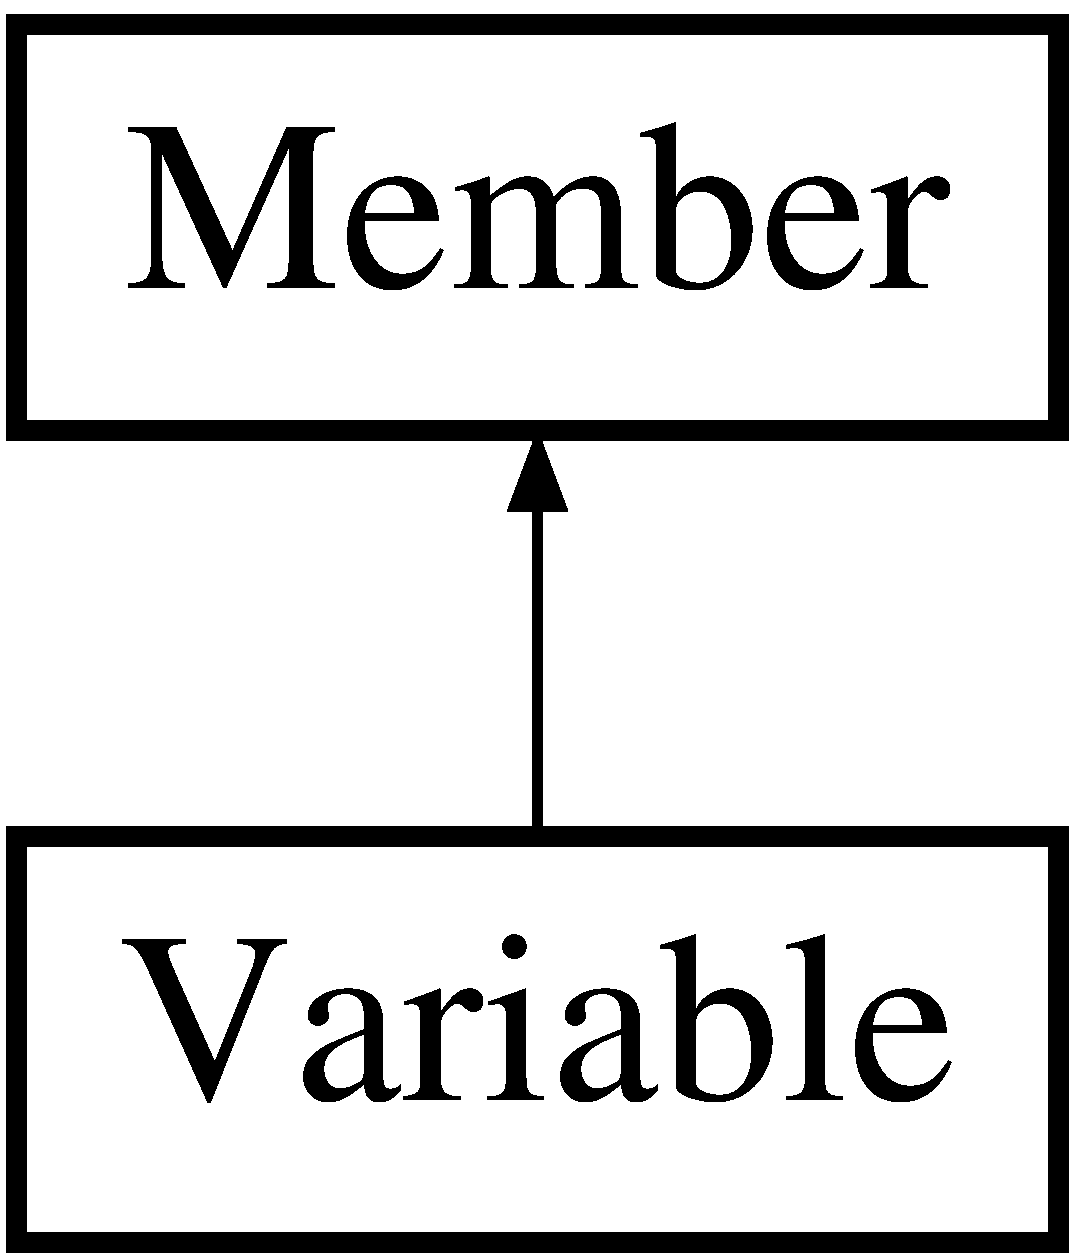
\includegraphics[height=2.000000cm]{classVariable}
\end{center}
\end{figure}
\subsection*{Public Member Functions}
\begin{DoxyCompactItemize}
\item 
\hypertarget{classVariable_a5716c9dcafcc8cf59a6f6b5dac3ec7a2}{\hyperlink{classVariable_a5716c9dcafcc8cf59a6f6b5dac3ec7a2}{Variable} ()}\label{classVariable_a5716c9dcafcc8cf59a6f6b5dac3ec7a2}

\begin{DoxyCompactList}\small\item\em Constructor. \end{DoxyCompactList}\item 
\hyperlink{classVariable_a9284a18cac758e26052f610a69b8921a}{Variable} (string name, vector$<$ \hyperlink{classType}{Type} $\ast$ $>$ types)
\begin{DoxyCompactList}\small\item\em Constructor. \end{DoxyCompactList}\item 
string \hyperlink{classVariable_a193be8605a472ddcceba928e746ffac2}{to\+\_\+string} ()
\begin{DoxyCompactList}\small\item\em Return a string that represent the variable. \end{DoxyCompactList}\item 
string \hyperlink{classVariable_aaebc8ef1594f951323e33725abfd69b5}{get\+Class} ()
\begin{DoxyCompactList}\small\item\em Return the name of the class. \end{DoxyCompactList}\end{DoxyCompactItemize}
\subsection*{Additional Inherited Members}


\subsection{Constructor \& Destructor Documentation}
\hypertarget{classVariable_a9284a18cac758e26052f610a69b8921a}{\index{Variable@{Variable}!Variable@{Variable}}
\index{Variable@{Variable}!Variable@{Variable}}
\subsubsection[{Variable}]{\setlength{\rightskip}{0pt plus 5cm}Variable\+::\+Variable (
\begin{DoxyParamCaption}
\item[{string}]{name, }
\item[{vector$<$ {\bf Type} $\ast$ $>$}]{types}
\end{DoxyParamCaption}
)}}\label{classVariable_a9284a18cac758e26052f610a69b8921a}


Constructor. 


\begin{DoxyParams}{Parameters}
{\em name} & -\/ name of the variable types -\/ either type of the variable \\
\hline
\end{DoxyParams}


\subsection{Member Function Documentation}
\hypertarget{classVariable_aaebc8ef1594f951323e33725abfd69b5}{\index{Variable@{Variable}!get\+Class@{get\+Class}}
\index{get\+Class@{get\+Class}!Variable@{Variable}}
\subsubsection[{get\+Class}]{\setlength{\rightskip}{0pt plus 5cm}string Variable\+::get\+Class (
\begin{DoxyParamCaption}
{}
\end{DoxyParamCaption}
)\hspace{0.3cm}{\ttfamily [virtual]}}}\label{classVariable_aaebc8ef1594f951323e33725abfd69b5}


Return the name of the class. 

\begin{DoxyReturn}{Returns}
\char`\"{}\+Variable\char`\"{} 
\end{DoxyReturn}


Reimplemented from \hyperlink{classMember_a7178ead1b2f1daa5fc5f993281ec90a4}{Member}.

\hypertarget{classVariable_a193be8605a472ddcceba928e746ffac2}{\index{Variable@{Variable}!to\+\_\+string@{to\+\_\+string}}
\index{to\+\_\+string@{to\+\_\+string}!Variable@{Variable}}
\subsubsection[{to\+\_\+string}]{\setlength{\rightskip}{0pt plus 5cm}string Variable\+::to\+\_\+string (
\begin{DoxyParamCaption}
{}
\end{DoxyParamCaption}
)\hspace{0.3cm}{\ttfamily [virtual]}}}\label{classVariable_a193be8605a472ddcceba928e746ffac2}


Return a string that represent the variable. 

\begin{DoxyReturn}{Returns}
a string \char`\"{} Variable name -\/ either type\char`\"{} 
\end{DoxyReturn}


Reimplemented from \hyperlink{classMember_aaa0028059dd87706188ee670bd28e4f2}{Member}.



The documentation for this class was generated from the following files\+:\begin{DoxyCompactItemize}
\item 
src/\hyperlink{variable_8h}{variable.\+h}\item 
src/\hyperlink{variable_8cpp}{variable.\+cpp}\end{DoxyCompactItemize}

\hypertarget{classVertex}{\section{Vertex Class Reference}
\label{classVertex}\index{Vertex@{Vertex}}
}
\subsection*{Public Member Functions}
\begin{DoxyCompactItemize}
\item 
\hypertarget{classVertex_a7ab79d72fd7da5b17ad2a96687f28330}{{\bfseries Vertex} (\hyperlink{classVertex}{Vertex} $\ast$father)}\label{classVertex_a7ab79d72fd7da5b17ad2a96687f28330}

\item 
\hypertarget{classVertex_ae7d9984499c01b2c04fd16a2e2bc6d23}{void {\bfseries add\+Action} (\hyperlink{classDurativeAction}{Durative\+Action} $\ast$action)}\label{classVertex_ae7d9984499c01b2c04fd16a2e2bc6d23}

\item 
\hypertarget{classVertex_a699b688b71b89946ee95177d9764730d}{void {\bfseries to\+\_\+string} ()}\label{classVertex_a699b688b71b89946ee95177d9764730d}

\item 
\hypertarget{classVertex_a6046d6709f420cd4cfa70f8ec0198a42}{vector$<$ \hyperlink{classDurativeAction}{Durative\+Action} $\ast$ $>$ $\ast$ {\bfseries get\+Actions} ()}\label{classVertex_a6046d6709f420cd4cfa70f8ec0198a42}

\item 
\hypertarget{classVertex_a8c56826133130f0fe0438ca066b8d35d}{\hyperlink{classVertex}{Vertex} $\ast$ {\bfseries get\+Father} ()}\label{classVertex_a8c56826133130f0fe0438ca066b8d35d}

\item 
\hypertarget{classVertex_a3ef7d7808ca40ae8841824aa47bd2e70}{void {\bfseries add\+Father} (\hyperlink{classVertex}{Vertex} $\ast$vertex)}\label{classVertex_a3ef7d7808ca40ae8841824aa47bd2e70}

\item 
\hypertarget{classVertex_aa535b74f28ae6e847243d85c1c53fb5a}{void {\bfseries add\+Actions} (vector$<$ \hyperlink{classDurativeAction}{Durative\+Action} $\ast$ $>$ $\ast$actions)}\label{classVertex_aa535b74f28ae6e847243d85c1c53fb5a}

\end{DoxyCompactItemize}


The documentation for this class was generated from the following files\+:\begin{DoxyCompactItemize}
\item 
src/vertex.\+h\item 
src/vertex.\+cpp\end{DoxyCompactItemize}

\chapter{File Documentation}
\hypertarget{Data_8cpp}{\section{Data.\+cpp File Reference}
\label{Data_8cpp}\index{Data.\+cpp@{Data.\+cpp}}
}


This class contains the data used by the parser generated with bisonc++ and flexc++.  


{\ttfamily \#include \char`\"{}Data.\+h\char`\"{}}\\*
{\ttfamily \#include $<$algorithm$>$}\\*
{\ttfamily \#include $<$iostream$>$}\\*


\subsection{Detailed Description}
This class contains the data used by the parser generated with bisonc++ and flexc++. 

\begin{DoxyAuthor}{Author}
Alan B\+E\+N\+I\+E\+R, Martin L\+A\+G\+L\+E\+I\+Z\+E, Nathan P\+R\+A\+T 
\end{DoxyAuthor}
\begin{DoxyVersion}{Version}
1.\+0 
\end{DoxyVersion}
\begin{DoxyDate}{Date}
May 07th 2014 
\end{DoxyDate}

\hypertarget{Data_8h}{\section{Data.\+h File Reference}
\label{Data_8h}\index{Data.\+h@{Data.\+h}}
}


This class contains the data used by the parser generated with bisonc++ and flexc++.  


{\ttfamily \#include $<$string$>$}\\*
{\ttfamily \#include $<$vector$>$}\\*
{\ttfamily \#include \char`\"{}src/attribute.\+h\char`\"{}}\\*
{\ttfamily \#include \char`\"{}src/predicate.\+h\char`\"{}}\\*
{\ttfamily \#include \char`\"{}src/constant.\+h\char`\"{}}\\*
{\ttfamily \#include \char`\"{}src/domain.\+h\char`\"{}}\\*
{\ttfamily \#include \char`\"{}src/durative\+\_\+action.\+h\char`\"{}}\\*
{\ttfamily \#include \char`\"{}src/fluent.\+h\char`\"{}}\\*
{\ttfamily \#include \char`\"{}src/function.\+h\char`\"{}}\\*
{\ttfamily \#include \char`\"{}src/interval.\+h\char`\"{}}\\*
{\ttfamily \#include \char`\"{}src/member.\+h\char`\"{}}\\*
{\ttfamily \#include \char`\"{}src/object.\+h\char`\"{}}\\*
{\ttfamily \#include \char`\"{}src/planning\+Data.\+h\char`\"{}}\\*
{\ttfamily \#include \char`\"{}src/problem.\+h\char`\"{}}\\*
{\ttfamily \#include \char`\"{}src/type.\+h\char`\"{}}\\*
{\ttfamily \#include \char`\"{}src/typed\+List.\+h\char`\"{}}\\*
{\ttfamily \#include \char`\"{}src/variable.\+h\char`\"{}}\\*
\subsection*{Classes}
\begin{DoxyCompactItemize}
\item 
class \hyperlink{classData}{Data}
\end{DoxyCompactItemize}


\subsection{Detailed Description}
This class contains the data used by the parser generated with bisonc++ and flexc++. 

\begin{DoxyAuthor}{Author}
Alan B\+E\+N\+I\+E\+R, Martin L\+A\+G\+L\+E\+I\+Z\+E, Nathan P\+R\+A\+T 
\end{DoxyAuthor}
\begin{DoxyVersion}{Version}
1.\+0 
\end{DoxyVersion}
\begin{DoxyDate}{Date}
May 07th 2014 
\end{DoxyDate}

\hypertarget{main_8cpp}{\section{main.\+cpp File Reference}
\label{main_8cpp}\index{main.\+cpp@{main.\+cpp}}
}


This program parse P\+D\+D\+L 3.\+1 T\+E domain and problem corresponding file, then it solve the planning problem following T\+L\+P-\/\+G\+P1 and T\+L\+P-\/\+G\+P2 algorithms.  


{\ttfamily \#include \char`\"{}parser/\+Parser.\+h\char`\"{}}\\*
{\ttfamily \#include $<$iostream$>$}\\*
{\ttfamily \#include $<$stdio.\+h$>$}\\*
{\ttfamily \#include $<$stdlib.\+h$>$}\\*
{\ttfamily \#include $<$string$>$}\\*
{\ttfamily \#include $<$unistd.\+h$>$}\\*
{\ttfamily \#include $<$time.\+h$>$}\\*
{\ttfamily \#include \char`\"{}src/graph.\+h\char`\"{}}\\*
{\ttfamily \#include \char`\"{}src/graph2.\+h\char`\"{}}\\*
{\ttfamily \#include \char`\"{}src/tlpgp1.\+h\char`\"{}}\\*
{\ttfamily \#include \char`\"{}src/tlpgp2.\+h\char`\"{}}\\*
\subsection*{Functions}
\begin{DoxyCompactItemize}
\item 
int \hyperlink{main_8cpp_a3c04138a5bfe5d72780bb7e82a18e627}{main} (int argc, char $\ast$$\ast$argv)
\begin{DoxyCompactList}\small\item\em This program parse P\+D\+D\+L 3.\+1 T\+E domain and problem corresponding file, then it solve the planning problem following T\+L\+P-\/\+G\+P1 and T\+L\+P-\/\+G\+P2 algorithms. \end{DoxyCompactList}\end{DoxyCompactItemize}
\subsection*{Variables}
\begin{DoxyCompactItemize}
\item 
\hypertarget{main_8cpp_adbe03f9636c37c0265219fe6fd049d50}{int {\bfseries g\+\_\+pid} = int(getpid())}\label{main_8cpp_adbe03f9636c37c0265219fe6fd049d50}

\end{DoxyCompactItemize}


\subsection{Detailed Description}
This program parse P\+D\+D\+L 3.\+1 T\+E domain and problem corresponding file, then it solve the planning problem following T\+L\+P-\/\+G\+P1 and T\+L\+P-\/\+G\+P2 algorithms. 

\begin{DoxyAuthor}{Author}
Alan B\+E\+N\+I\+E\+R, Martin L\+A\+G\+L\+E\+I\+Z\+E, Nathan P\+R\+A\+T 
\end{DoxyAuthor}
\begin{DoxyVersion}{Version}
1.\+0 
\end{DoxyVersion}
\begin{DoxyDate}{Date}
May 07th 2014 
\end{DoxyDate}


\subsection{Function Documentation}
\hypertarget{main_8cpp_a3c04138a5bfe5d72780bb7e82a18e627}{\index{main.\+cpp@{main.\+cpp}!main@{main}}
\index{main@{main}!main.\+cpp@{main.\+cpp}}
\subsubsection[{main}]{\setlength{\rightskip}{0pt plus 5cm}int main (
\begin{DoxyParamCaption}
\item[{int}]{argc, }
\item[{char $\ast$$\ast$}]{argv}
\end{DoxyParamCaption}
)}}\label{main_8cpp_a3c04138a5bfe5d72780bb7e82a18e627}


This program parse P\+D\+D\+L 3.\+1 T\+E domain and problem corresponding file, then it solve the planning problem following T\+L\+P-\/\+G\+P1 and T\+L\+P-\/\+G\+P2 algorithms. 


\begin{DoxyParams}{Parameters}
{\em domain\+File.\+pddl} & problem\+File.\+pddl \\
\hline
\end{DoxyParams}
\begin{DoxyReturn}{Returns}
Print the result of the planner on stdout 
\end{DoxyReturn}

\hypertarget{Parser_8h}{\section{parser/\+Parser.h File Reference}
\label{Parser_8h}\index{parser/\+Parser.\+h@{parser/\+Parser.\+h}}
}


This file have been generated by bisonc++ and completed by us.  


{\ttfamily \#include \char`\"{}Parserbase.\+h\char`\"{}}\\*
{\ttfamily \#include \char`\"{}../scanner/\+Scanner.\+h\char`\"{}}\\*
{\ttfamily \#include \char`\"{}../headers.\+h\char`\"{}}\\*
\subsection*{Classes}
\begin{DoxyCompactItemize}
\item 
class \hyperlink{classParser}{Parser}
\end{DoxyCompactItemize}


\subsection{Detailed Description}
This file have been generated by bisonc++ and completed by us. 

\begin{DoxyAuthor}{Author}
Alan B\+E\+N\+I\+E\+R, Martin L\+A\+G\+L\+E\+I\+Z\+E, Nathan P\+R\+A\+T 
\end{DoxyAuthor}
\begin{DoxyVersion}{Version}
1.\+0 
\end{DoxyVersion}
\begin{DoxyDate}{Date}
May 07th 2014 
\end{DoxyDate}

\hypertarget{attribute_8cpp}{\section{src/attribute.cpp File Reference}
\label{attribute_8cpp}\index{src/attribute.\+cpp@{src/attribute.\+cpp}}
}


This class represent a P\+D\+D\+L Temporally Extended attribute (invented by Frederic Maris), which are the main feature of the interval of preconditions and effects of P\+D\+D\+L durative-\/actions.  


{\ttfamily \#include \char`\"{}attribute.\+h\char`\"{}}\\*


\subsection{Detailed Description}
This class represent a P\+D\+D\+L Temporally Extended attribute (invented by Frederic Maris), which are the main feature of the interval of preconditions and effects of P\+D\+D\+L durative-\/actions. 

\begin{DoxyAuthor}{Author}
Alan B\+E\+N\+I\+E\+R, Martin L\+A\+G\+L\+E\+I\+Z\+E, Nathan P\+R\+A\+T 
\end{DoxyAuthor}
\begin{DoxyVersion}{Version}
1.\+0 
\end{DoxyVersion}
\begin{DoxyDate}{Date}
May 07th 2014 
\end{DoxyDate}

\hypertarget{attribute_8h}{\section{src/attribute.h File Reference}
\label{attribute_8h}\index{src/attribute.\+h@{src/attribute.\+h}}
}


This class represent a P\+D\+D\+L Temporally Extended attribute (invented by Frederic Maris), which are the main feature of the interval of preconditions and effects of P\+D\+D\+L durative-\/actions.  


{\ttfamily \#include $<$string$>$}\\*
{\ttfamily \#include $<$vector$>$}\\*
{\ttfamily \#include \char`\"{}interval.\+h\char`\"{}}\\*
\subsection*{Classes}
\begin{DoxyCompactItemize}
\item 
class \hyperlink{classAttribute}{Attribute}
\end{DoxyCompactItemize}


\subsection{Detailed Description}
This class represent a P\+D\+D\+L Temporally Extended attribute (invented by Frederic Maris), which are the main feature of the interval of preconditions and effects of P\+D\+D\+L durative-\/actions. 

\begin{DoxyAuthor}{Author}
Alan B\+E\+N\+I\+E\+R, Martin L\+A\+G\+L\+E\+I\+Z\+E, Nathan P\+R\+A\+T 
\end{DoxyAuthor}
\begin{DoxyVersion}{Version}
1.\+0 
\end{DoxyVersion}
\begin{DoxyDate}{Date}
May 07th 2014 
\end{DoxyDate}

\hypertarget{constant_8cpp}{\section{src/constant.cpp File Reference}
\label{constant_8cpp}\index{src/constant.\+cpp@{src/constant.\+cpp}}
}


This class represent a P\+D\+D\+L constant, inherit from \hyperlink{classMember}{Member}.  


{\ttfamily \#include \char`\"{}constant.\+h\char`\"{}}\\*


\subsection{Detailed Description}
This class represent a P\+D\+D\+L constant, inherit from \hyperlink{classMember}{Member}. 

\begin{DoxyAuthor}{Author}
Alan B\+E\+N\+I\+E\+R, Martin L\+A\+G\+L\+E\+I\+Z\+E, Nathan P\+R\+A\+T 
\end{DoxyAuthor}
\begin{DoxyVersion}{Version}
1.\+0 
\end{DoxyVersion}
\begin{DoxyDate}{Date}
May 07th 2014 
\end{DoxyDate}

\hypertarget{constant_8h}{\section{src/constant.h File Reference}
\label{constant_8h}\index{src/constant.\+h@{src/constant.\+h}}
}


This class represent a P\+D\+D\+L constant, inherit from \hyperlink{classMember}{Member}.  


{\ttfamily \#include \char`\"{}member.\+h\char`\"{}}\\*
\subsection*{Classes}
\begin{DoxyCompactItemize}
\item 
class \hyperlink{classConstant}{Constant}
\end{DoxyCompactItemize}


\subsection{Detailed Description}
This class represent a P\+D\+D\+L constant, inherit from \hyperlink{classMember}{Member}. 

\begin{DoxyAuthor}{Author}
Alan B\+E\+N\+I\+E\+R, Martin L\+A\+G\+L\+E\+I\+Z\+E, Nathan P\+R\+A\+T 
\end{DoxyAuthor}
\begin{DoxyVersion}{Version}
1.\+0 
\end{DoxyVersion}
\begin{DoxyDate}{Date}
May 07th 2014 
\end{DoxyDate}

\hypertarget{constraint_8cpp}{\section{src/constraint.cpp File Reference}
\label{constraint_8cpp}\index{src/constraint.\+cpp@{src/constraint.\+cpp}}
}


\mbox{[}wip\mbox{]}\mbox{[}test\mbox{]} contains things which may be used in tlpgp1  


{\ttfamily \#include \char`\"{}constraint.\+h\char`\"{}}\\*


\subsection{Detailed Description}
\mbox{[}wip\mbox{]}\mbox{[}test\mbox{]} contains things which may be used in tlpgp1 

\begin{DoxyAuthor}{Author}
Alan B\+E\+N\+I\+E\+R, Martin L\+A\+G\+L\+E\+I\+Z\+E, Nathan P\+R\+A\+T 
\end{DoxyAuthor}
\begin{DoxyVersion}{Version}
1.\+0 
\end{DoxyVersion}
\begin{DoxyDate}{Date}
Apr 18, 2014 
\end{DoxyDate}

\hypertarget{constraint_8h}{\section{src/constraint.h File Reference}
\label{constraint_8h}\index{src/constraint.\+h@{src/constraint.\+h}}
}


\mbox{[}wip\mbox{]}\mbox{[}test\mbox{]} contains things which may be used in tlpgp1  


{\ttfamily \#include $<$iostream$>$}\\*
{\ttfamily \#include $<$stdio.\+h$>$}\\*
{\ttfamily \#include $<$stdlib.\+h$>$}\\*
{\ttfamily \#include $<$string$>$}\\*
{\ttfamily \#include $<$unistd.\+h$>$}\\*
{\ttfamily \#include $<$vector$>$}\\*
{\ttfamily \#include \char`\"{}../\+Data.\+h\char`\"{}}\\*
{\ttfamily \#include \char`\"{}problem.\+h\char`\"{}}\\*
{\ttfamily \#include \char`\"{}domain.\+h\char`\"{}}\\*
\subsection*{Classes}
\begin{DoxyCompactItemize}
\item 
class \hyperlink{classstd_1_1constraint}{std\+::constraint}
\end{DoxyCompactItemize}


\subsection{Detailed Description}
\mbox{[}wip\mbox{]}\mbox{[}test\mbox{]} contains things which may be used in tlpgp1 

\begin{DoxyAuthor}{Author}
Alan B\+E\+N\+I\+E\+R, Martin L\+A\+G\+L\+E\+I\+Z\+E, Nathan P\+R\+A\+T 
\end{DoxyAuthor}
\begin{DoxyVersion}{Version}
1.\+0 
\end{DoxyVersion}
\begin{DoxyDate}{Date}
Apr 18, 2014 
\end{DoxyDate}

\hypertarget{fluent_8cpp}{\section{src/fluent.cpp File Reference}
\label{fluent_8cpp}\index{src/fluent.\+cpp@{src/fluent.\+cpp}}
}


This class represent a fluent, which is a predicate of which parameters have been set.  


{\ttfamily \#include \char`\"{}fluent.\+h\char`\"{}}\\*


\subsection{Detailed Description}
This class represent a fluent, which is a predicate of which parameters have been set. 

\begin{DoxyAuthor}{Author}
Alan B\+E\+N\+I\+E\+R, Martin L\+A\+G\+L\+E\+I\+Z\+E, Nathan P\+R\+A\+T 
\end{DoxyAuthor}
\begin{DoxyVersion}{Version}
1.\+0 
\end{DoxyVersion}
\begin{DoxyDate}{Date}
May 07th 2014 
\end{DoxyDate}

\hypertarget{fluent_8h}{\section{src/fluent.h File Reference}
\label{fluent_8h}\index{src/fluent.\+h@{src/fluent.\+h}}
}


This class represent a fluent, which is a predicate of which parameters have been set.  


{\ttfamily \#include $<$string$>$}\\*
{\ttfamily \#include $<$vector$>$}\\*
{\ttfamily \#include \char`\"{}member.\+h\char`\"{}}\\*
{\ttfamily \#include \char`\"{}predicate.\+h\char`\"{}}\\*
\subsection*{Classes}
\begin{DoxyCompactItemize}
\item 
class \hyperlink{classFluent}{Fluent}
\end{DoxyCompactItemize}


\subsection{Detailed Description}
This class represent a fluent, which is a predicate of which parameters have been set. 

\begin{DoxyAuthor}{Author}
Alan B\+E\+N\+I\+E\+R, Martin L\+A\+G\+L\+E\+I\+Z\+E, Nathan P\+R\+A\+T 
\end{DoxyAuthor}
\begin{DoxyVersion}{Version}
1.\+0 
\end{DoxyVersion}
\begin{DoxyDate}{Date}
May 07th 2014 
\end{DoxyDate}

\hypertarget{function_8cpp}{\section{src/function.cpp File Reference}
\label{function_8cpp}\index{src/function.\+cpp@{src/function.\+cpp}}
}


This class represent a P\+D\+D\+L function.  


{\ttfamily \#include \char`\"{}function.\+h\char`\"{}}\\*


\subsection{Detailed Description}
This class represent a P\+D\+D\+L function. 

\begin{DoxyAuthor}{Author}
Alan B\+E\+N\+I\+E\+R, Martin L\+A\+G\+L\+E\+I\+Z\+E, Nathan P\+R\+A\+T 
\end{DoxyAuthor}
\begin{DoxyVersion}{Version}
1.\+0 
\end{DoxyVersion}
\begin{DoxyDate}{Date}
May 07th 2014 
\end{DoxyDate}

\hypertarget{function_8h}{\section{src/function.h File Reference}
\label{function_8h}\index{src/function.\+h@{src/function.\+h}}
}


This class represent a P\+D\+D\+L function.  


{\ttfamily \#include $<$string$>$}\\*
{\ttfamily \#include $<$vector$>$}\\*
{\ttfamily \#include \char`\"{}type.\+h\char`\"{}}\\*
\subsection*{Classes}
\begin{DoxyCompactItemize}
\item 
class \hyperlink{classFunction}{Function}
\end{DoxyCompactItemize}


\subsection{Detailed Description}
This class represent a P\+D\+D\+L function. 

\begin{DoxyAuthor}{Author}
Alan B\+E\+N\+I\+E\+R, Martin L\+A\+G\+L\+E\+I\+Z\+E, Nathan P\+R\+A\+T 
\end{DoxyAuthor}
\begin{DoxyVersion}{Version}
1.\+0 
\end{DoxyVersion}
\begin{DoxyDate}{Date}
May 07th 2014 
\end{DoxyDate}

\hypertarget{graph2_8cpp}{\section{src/graph2.cpp File Reference}
\label{graph2_8cpp}\index{src/graph2.\+cpp@{src/graph2.\+cpp}}
}


Contains what is needed to generate the expansion graph for tlpgp1.  


{\ttfamily \#include \char`\"{}graph2.\+h\char`\"{}}\\*


\subsection{Detailed Description}
Contains what is needed to generate the expansion graph for tlpgp1. 

\begin{DoxyAuthor}{Author}
Alan B\+E\+N\+I\+E\+R, Martin L\+A\+G\+L\+E\+I\+Z\+E, Nathan P\+R\+A\+T 
\end{DoxyAuthor}
\begin{DoxyVersion}{Version}
1.\+0 
\end{DoxyVersion}
\begin{DoxyDate}{Date}
May 6, 2014 basically Copy-\/pasted from graph.\+cpp 
\end{DoxyDate}

\hypertarget{graph2_8h}{\section{src/graph2.h File Reference}
\label{graph2_8h}\index{src/graph2.\+h@{src/graph2.\+h}}
}


Contains what is needed to generate the expansion graph for tlpgp1.  


{\ttfamily \#include $<$iostream$>$}\\*
{\ttfamily \#include $<$stdio.\+h$>$}\\*
{\ttfamily \#include $<$stdlib.\+h$>$}\\*
{\ttfamily \#include $<$string$>$}\\*
{\ttfamily \#include $<$unistd.\+h$>$}\\*
{\ttfamily \#include $<$vector$>$}\\*
{\ttfamily \#include \char`\"{}../\+Data.\+h\char`\"{}}\\*
{\ttfamily \#include \char`\"{}problem.\+h\char`\"{}}\\*
{\ttfamily \#include \char`\"{}domain.\+h\char`\"{}}\\*
{\ttfamily \#include \char`\"{}edge.\+h\char`\"{}}\\*
{\ttfamily \#include \char`\"{}vertex.\+h\char`\"{}}\\*
{\ttfamily \#include \char`\"{}tools.\+h\char`\"{}}\\*
{\ttfamily \#include \char`\"{}l\+Obj\+Type.\+h\char`\"{}}\\*
{\ttfamily \#include \char`\"{}constraint.\+h\char`\"{}}\\*
{\ttfamily \#include \char`\"{}sat.\+h\char`\"{}}\\*
{\ttfamily \#include \char`\"{}attribute.\+h\char`\"{}}\\*
{\ttfamily \#include \char`\"{}tlpgp2.\+h\char`\"{}}\\*
\subsection*{Classes}
\begin{DoxyCompactItemize}
\item 
class \hyperlink{classGraph2}{Graph2}
\end{DoxyCompactItemize}


\subsection{Detailed Description}
Contains what is needed to generate the expansion graph for tlpgp1. 

\begin{DoxyAuthor}{Author}
Alan B\+E\+N\+I\+E\+R, Martin L\+A\+G\+L\+E\+I\+Z\+E, Nathan P\+R\+A\+T 
\end{DoxyAuthor}
\begin{DoxyVersion}{Version}
1.\+0 
\end{DoxyVersion}
\begin{DoxyDate}{Date}
May 6, 2014 basically Copy-\/pasted from graph.\+cpp 
\end{DoxyDate}

\hypertarget{interval_8cpp}{\section{src/interval.cpp File Reference}
\label{interval_8cpp}\index{src/interval.\+cpp@{src/interval.\+cpp}}
}


This class represent an interval of which bounds are floats.  


{\ttfamily \#include \char`\"{}interval.\+h\char`\"{}}\\*
{\ttfamily \#include $<$sstream$>$}\\*
\subsection*{Functions}
\begin{DoxyCompactItemize}
\item 
\hypertarget{interval_8cpp_a851fefcccd92000966209f54cabce221}{{\footnotesize template$<$typename T $>$ }\\string {\bfseries tostr} (const T \&t)}\label{interval_8cpp_a851fefcccd92000966209f54cabce221}

\end{DoxyCompactItemize}


\subsection{Detailed Description}
This class represent an interval of which bounds are floats. 

\begin{DoxyAuthor}{Author}
Alan B\+E\+N\+I\+E\+R, Martin L\+A\+G\+L\+E\+I\+Z\+E, Nathan P\+R\+A\+T 
\end{DoxyAuthor}
\begin{DoxyVersion}{Version}
1.\+0 
\end{DoxyVersion}
\begin{DoxyDate}{Date}
May 07th 2014 
\end{DoxyDate}

\hypertarget{interval_8h}{\section{src/interval.h File Reference}
\label{interval_8h}\index{src/interval.\+h@{src/interval.\+h}}
}


This class represent an interval of which bounds are floats.  


{\ttfamily \#include $<$string$>$}\\*
\subsection*{Classes}
\begin{DoxyCompactItemize}
\item 
class \hyperlink{classInterval}{Interval}
\end{DoxyCompactItemize}


\subsection{Detailed Description}
This class represent an interval of which bounds are floats. 

\begin{DoxyAuthor}{Author}
Alan B\+E\+N\+I\+E\+R, Martin L\+A\+G\+L\+E\+I\+Z\+E, Nathan P\+R\+A\+T 
\end{DoxyAuthor}
\begin{DoxyVersion}{Version}
1.\+0 
\end{DoxyVersion}
\begin{DoxyDate}{Date}
May 07th 2014 
\end{DoxyDate}

\hypertarget{member_8cpp}{\section{src/member.cpp File Reference}
\label{member_8cpp}\index{src/member.\+cpp@{src/member.\+cpp}}
}


This class represent a P\+D\+D\+L constant, object or variable.  


{\ttfamily \#include \char`\"{}member.\+h\char`\"{}}\\*


\subsection{Detailed Description}
This class represent a P\+D\+D\+L constant, object or variable. 

\begin{DoxyAuthor}{Author}
Alan B\+E\+N\+I\+E\+R, Martin L\+A\+G\+L\+E\+I\+Z\+E, Nathan P\+R\+A\+T 
\end{DoxyAuthor}
\begin{DoxyVersion}{Version}
1.\+0 
\end{DoxyVersion}
\begin{DoxyDate}{Date}
May 07th 2014 
\end{DoxyDate}

\hypertarget{member_8h}{\section{src/member.h File Reference}
\label{member_8h}\index{src/member.\+h@{src/member.\+h}}
}


This class represent a P\+D\+D\+L constant, object or variable.  


{\ttfamily \#include $<$string$>$}\\*
{\ttfamily \#include $<$vector$>$}\\*
{\ttfamily \#include \char`\"{}type.\+h\char`\"{}}\\*
\subsection*{Classes}
\begin{DoxyCompactItemize}
\item 
class \hyperlink{classMember}{Member}
\end{DoxyCompactItemize}


\subsection{Detailed Description}
This class represent a P\+D\+D\+L constant, object or variable. 

\begin{DoxyAuthor}{Author}
Alan B\+E\+N\+I\+E\+R, Martin L\+A\+G\+L\+E\+I\+Z\+E, Nathan P\+R\+A\+T 
\end{DoxyAuthor}
\begin{DoxyVersion}{Version}
1.\+0 
\end{DoxyVersion}
\begin{DoxyDate}{Date}
May 07th 2014 
\end{DoxyDate}

\hypertarget{object_8h}{\section{src/object.h File Reference}
\label{object_8h}\index{src/object.\+h@{src/object.\+h}}
}


This class represent a P\+D\+D\+L object, inherit from \hyperlink{classMember}{Member}.  


{\ttfamily \#include \char`\"{}member.\+h\char`\"{}}\\*
\subsection*{Classes}
\begin{DoxyCompactItemize}
\item 
class \hyperlink{classObject}{Object}
\end{DoxyCompactItemize}


\subsection{Detailed Description}
This class represent a P\+D\+D\+L object, inherit from \hyperlink{classMember}{Member}. 

\begin{DoxyAuthor}{Author}
Alan B\+E\+N\+I\+E\+R, Martin L\+A\+G\+L\+E\+I\+Z\+E, Nathan P\+R\+A\+T 
\end{DoxyAuthor}
\begin{DoxyVersion}{Version}
1.\+0 
\end{DoxyVersion}
\begin{DoxyDate}{Date}
May 07th 2014 
\end{DoxyDate}

\hypertarget{predicate_8cpp}{\section{src/predicate.cpp File Reference}
\label{predicate_8cpp}\index{src/predicate.\+cpp@{src/predicate.\+cpp}}
}


This class represent a P\+D\+D\+L predicate.  


{\ttfamily \#include \char`\"{}predicate.\+h\char`\"{}}\\*


\subsection{Detailed Description}
This class represent a P\+D\+D\+L predicate. 

\begin{DoxyAuthor}{Author}
Alan B\+E\+N\+I\+E\+R, Martin L\+A\+G\+L\+E\+I\+Z\+E, Nathan P\+R\+A\+T 
\end{DoxyAuthor}
\begin{DoxyVersion}{Version}
1.\+0 
\end{DoxyVersion}
\begin{DoxyDate}{Date}
May 07th 2014 
\end{DoxyDate}

\hypertarget{predicate_8h}{\section{src/predicate.h File Reference}
\label{predicate_8h}\index{src/predicate.\+h@{src/predicate.\+h}}
}


This class represent a P\+D\+D\+L predicate.  


{\ttfamily \#include $<$string$>$}\\*
{\ttfamily \#include $<$vector$>$}\\*
{\ttfamily \#include \char`\"{}type.\+h\char`\"{}}\\*
\subsection*{Classes}
\begin{DoxyCompactItemize}
\item 
class \hyperlink{classPredicate}{Predicate}
\end{DoxyCompactItemize}


\subsection{Detailed Description}
This class represent a P\+D\+D\+L predicate. 

\begin{DoxyAuthor}{Author}
Alan B\+E\+N\+I\+E\+R, Martin L\+A\+G\+L\+E\+I\+Z\+E, Nathan P\+R\+A\+T 
\end{DoxyAuthor}
\begin{DoxyVersion}{Version}
1.\+0 
\end{DoxyVersion}
\begin{DoxyDate}{Date}
May 07th 2014 
\end{DoxyDate}

\hypertarget{sat_8cpp}{\section{src/sat.cpp File Reference}
\label{sat_8cpp}\index{src/sat.\+cpp@{src/sat.\+cpp}}
}


contains what is needed to communicate with a sat solver, using smt2  


{\ttfamily \#include \char`\"{}sat.\+h\char`\"{}}\\*


\subsection{Detailed Description}
contains what is needed to communicate with a sat solver, using smt2 

\begin{DoxyAuthor}{Author}
Alan B\+E\+N\+I\+E\+R, Martin L\+A\+G\+L\+E\+I\+Z\+E, Nathan P\+R\+A\+T 
\end{DoxyAuthor}
\begin{DoxyVersion}{Version}
1.\+0 
\end{DoxyVersion}
\begin{DoxyDate}{Date}
Apr 20, 2014 
\end{DoxyDate}

\hypertarget{sat_8h}{\section{src/sat.h File Reference}
\label{sat_8h}\index{src/sat.\+h@{src/sat.\+h}}
}


contains what is needed to communicate with a sat solver, using smt2  


{\ttfamily \#include $<$iostream$>$}\\*
{\ttfamily \#include $<$fstream$>$}\\*
{\ttfamily \#include $<$stdio.\+h$>$}\\*
{\ttfamily \#include $<$stdlib.\+h$>$}\\*
{\ttfamily \#include $<$string$>$}\\*
{\ttfamily \#include $<$unistd.\+h$>$}\\*
\subsection*{Classes}
\begin{DoxyCompactItemize}
\item 
class \hyperlink{classSat}{Sat}
\end{DoxyCompactItemize}


\subsection{Detailed Description}
contains what is needed to communicate with a sat solver, using smt2 

\begin{DoxyAuthor}{Author}
Alan B\+E\+N\+I\+E\+R, Martin L\+A\+G\+L\+E\+I\+Z\+E, Nathan P\+R\+A\+T 
\end{DoxyAuthor}
\begin{DoxyVersion}{Version}
1.\+0 
\end{DoxyVersion}
\begin{DoxyDate}{Date}
Apr 20, 2014 
\end{DoxyDate}

\hypertarget{tlpgp1_8cpp}{\section{src/tlpgp1.cpp File Reference}
\label{tlpgp1_8cpp}\index{src/tlpgp1.\+cpp@{src/tlpgp1.\+cpp}}
}


\mbox{[}wip\mbox{]}Contains the core code of tlpgp1  


{\ttfamily \#include \char`\"{}tlpgp1.\+h\char`\"{}}\\*


\subsection{Detailed Description}
\mbox{[}wip\mbox{]}Contains the core code of tlpgp1 

\begin{DoxyAuthor}{Author}
Alan B\+E\+N\+I\+E\+R, Martin L\+A\+G\+L\+E\+I\+Z\+E, Nathan P\+R\+A\+T 
\end{DoxyAuthor}
\begin{DoxyVersion}{Version}
1.\+0 
\end{DoxyVersion}
\begin{DoxyDate}{Date}
Apr 23, 2014 
\end{DoxyDate}

\hypertarget{tlpgp1_8h}{\section{src/tlpgp1.h File Reference}
\label{tlpgp1_8h}\index{src/tlpgp1.\+h@{src/tlpgp1.\+h}}
}


Contains the core code of tlpgp1.  


{\ttfamily \#include $<$iostream$>$}\\*
{\ttfamily \#include $<$stdio.\+h$>$}\\*
{\ttfamily \#include $<$stdlib.\+h$>$}\\*
{\ttfamily \#include $<$string$>$}\\*
{\ttfamily \#include $<$unistd.\+h$>$}\\*
{\ttfamily \#include $<$vector$>$}\\*
{\ttfamily \#include $<$algorithm$>$}\\*
{\ttfamily \#include \char`\"{}../\+Data.\+h\char`\"{}}\\*
{\ttfamily \#include \char`\"{}problem.\+h\char`\"{}}\\*
{\ttfamily \#include \char`\"{}domain.\+h\char`\"{}}\\*
{\ttfamily \#include \char`\"{}edge.\+h\char`\"{}}\\*
{\ttfamily \#include \char`\"{}vertex.\+h\char`\"{}}\\*
{\ttfamily \#include \char`\"{}tools.\+h\char`\"{}}\\*
{\ttfamily \#include \char`\"{}l\+Obj\+Type.\+h\char`\"{}}\\*
{\ttfamily \#include \char`\"{}constraint.\+h\char`\"{}}\\*
{\ttfamily \#include \char`\"{}sat.\+h\char`\"{}}\\*
{\ttfamily \#include \char`\"{}graph2.\+h\char`\"{}}\\*
\subsection*{Classes}
\begin{DoxyCompactItemize}
\item 
class \hyperlink{classTlpgp1}{Tlpgp1}
\end{DoxyCompactItemize}


\subsection{Detailed Description}
Contains the core code of tlpgp1. 

\begin{DoxyAuthor}{Author}
Alan B\+E\+N\+I\+E\+R, Martin L\+A\+G\+L\+E\+I\+Z\+E, Nathan P\+R\+A\+T 
\end{DoxyAuthor}
\begin{DoxyVersion}{Version}
1.\+0 
\end{DoxyVersion}
\begin{DoxyDate}{Date}
Apr 23, 2014 
\end{DoxyDate}

\hypertarget{type_8cpp}{\section{src/type.cpp File Reference}
\label{type_8cpp}\index{src/type.\+cpp@{src/type.\+cpp}}
}


This class represent a P\+D\+D\+L type.  


{\ttfamily \#include \char`\"{}type.\+h\char`\"{}}\\*
{\ttfamily \#include $<$iostream$>$}\\*


\subsection{Detailed Description}
This class represent a P\+D\+D\+L type. 

\begin{DoxyAuthor}{Author}
Alan B\+E\+N\+I\+E\+R, Martin L\+A\+G\+L\+E\+I\+Z\+E, Nathan P\+R\+A\+T 
\end{DoxyAuthor}
\begin{DoxyVersion}{Version}
1.\+0 
\end{DoxyVersion}
\begin{DoxyDate}{Date}
May 07th 2014 
\end{DoxyDate}

\hypertarget{type_8h}{\section{src/type.h File Reference}
\label{type_8h}\index{src/type.\+h@{src/type.\+h}}
}


This class represent a P\+D\+D\+L type.  


{\ttfamily \#include $<$string$>$}\\*
{\ttfamily \#include $<$vector$>$}\\*
\subsection*{Classes}
\begin{DoxyCompactItemize}
\item 
class \hyperlink{classType}{Type}
\end{DoxyCompactItemize}


\subsection{Detailed Description}
This class represent a P\+D\+D\+L type. 

\begin{DoxyAuthor}{Author}
Alan B\+E\+N\+I\+E\+R, Martin L\+A\+G\+L\+E\+I\+Z\+E, Nathan P\+R\+A\+T 
\end{DoxyAuthor}
\begin{DoxyVersion}{Version}
1.\+0 
\end{DoxyVersion}
\begin{DoxyDate}{Date}
May 07th 2014 
\end{DoxyDate}

\hypertarget{typedList_8cpp}{\section{src/typed\+List.cpp File Reference}
\label{typedList_8cpp}\index{src/typed\+List.\+cpp@{src/typed\+List.\+cpp}}
}


This class represent a parser's typed\+List, which is a pair of a list of name and an either type.  


{\ttfamily \#include \char`\"{}typed\+List.\+h\char`\"{}}\\*


\subsection{Detailed Description}
This class represent a parser's typed\+List, which is a pair of a list of name and an either type. 

\begin{DoxyAuthor}{Author}
Alan B\+E\+N\+I\+E\+R, Martin L\+A\+G\+L\+E\+I\+Z\+E, Nathan P\+R\+A\+T 
\end{DoxyAuthor}
\begin{DoxyVersion}{Version}
1.\+0 
\end{DoxyVersion}
\begin{DoxyDate}{Date}
May 07th 2014 
\end{DoxyDate}

\hypertarget{typedList_8h}{\section{src/typed\+List.h File Reference}
\label{typedList_8h}\index{src/typed\+List.\+h@{src/typed\+List.\+h}}
}


This class represent a parser's typed\+List, which is a pair of a list of name and an either type.  


{\ttfamily \#include $<$string$>$}\\*
{\ttfamily \#include $<$vector$>$}\\*
{\ttfamily \#include \char`\"{}type.\+h\char`\"{}}\\*
\subsection*{Classes}
\begin{DoxyCompactItemize}
\item 
class \hyperlink{classTypedList}{Typed\+List}
\end{DoxyCompactItemize}


\subsection{Detailed Description}
This class represent a parser's typed\+List, which is a pair of a list of name and an either type. 

\begin{DoxyAuthor}{Author}
Alan B\+E\+N\+I\+E\+R, Martin L\+A\+G\+L\+E\+I\+Z\+E, Nathan P\+R\+A\+T 
\end{DoxyAuthor}
\begin{DoxyVersion}{Version}
1.\+0 
\end{DoxyVersion}
\begin{DoxyDate}{Date}
May 07th 2014 
\end{DoxyDate}

\hypertarget{variable_8cpp}{\section{src/variable.cpp File Reference}
\label{variable_8cpp}\index{src/variable.\+cpp@{src/variable.\+cpp}}
}


This class represent a P\+D\+D\+L variable, inherit from \hyperlink{classMember}{Member}.  


{\ttfamily \#include \char`\"{}variable.\+h\char`\"{}}\\*


\subsection{Detailed Description}
This class represent a P\+D\+D\+L variable, inherit from \hyperlink{classMember}{Member}. 

\begin{DoxyAuthor}{Author}
Alan B\+E\+N\+I\+E\+R, Martin L\+A\+G\+L\+E\+I\+Z\+E, Nathan P\+R\+A\+T 
\end{DoxyAuthor}
\begin{DoxyVersion}{Version}
1.\+0 
\end{DoxyVersion}
\begin{DoxyDate}{Date}
May 07th 2014 
\end{DoxyDate}

\hypertarget{variable_8h}{\section{src/variable.h File Reference}
\label{variable_8h}\index{src/variable.\+h@{src/variable.\+h}}
}


This class represent a P\+D\+D\+L variable, inherit from \hyperlink{classMember}{Member}.  


{\ttfamily \#include \char`\"{}member.\+h\char`\"{}}\\*
\subsection*{Classes}
\begin{DoxyCompactItemize}
\item 
class \hyperlink{classVariable}{Variable}
\end{DoxyCompactItemize}


\subsection{Detailed Description}
This class represent a P\+D\+D\+L variable, inherit from \hyperlink{classMember}{Member}. 

\begin{DoxyAuthor}{Author}
Alan B\+E\+N\+I\+E\+R, Martin L\+A\+G\+L\+E\+I\+Z\+E, Nathan P\+R\+A\+T 
\end{DoxyAuthor}
\begin{DoxyVersion}{Version}
1.\+0 
\end{DoxyVersion}
\begin{DoxyDate}{Date}
May 07th 2014 
\end{DoxyDate}

%--- End generated contents ---

% Index
\newpage
\phantomsection
\addcontentsline{toc}{chapter}{Index}
\printindex

\end{document}
